\documentclass[twoside]{book}

% Packages required by doxygen
\usepackage{fixltx2e}
\usepackage{calc}
\usepackage{doxygen}
\usepackage[export]{adjustbox} % also loads graphicx
\usepackage{graphicx}
\usepackage[utf8]{inputenc}
\usepackage{makeidx}
\usepackage{multicol}
\usepackage{multirow}
\PassOptionsToPackage{warn}{textcomp}
\usepackage{textcomp}
\usepackage[nointegrals]{wasysym}
\usepackage[table]{xcolor}

% Font selection
\usepackage[T1]{fontenc}
\usepackage[scaled=.90]{helvet}
\usepackage{courier}
\usepackage{amssymb}
\usepackage{sectsty}
\renewcommand{\familydefault}{\sfdefault}
\allsectionsfont{%
  \fontseries{bc}\selectfont%
  \color{darkgray}%
}
\renewcommand{\DoxyLabelFont}{%
  \fontseries{bc}\selectfont%
  \color{darkgray}%
}
\newcommand{\+}{\discretionary{\mbox{\scriptsize$\hookleftarrow$}}{}{}}

% Page & text layout
\usepackage{geometry}
\geometry{%
  a4paper,%
  top=2.5cm,%
  bottom=2.5cm,%
  left=2.5cm,%
  right=2.5cm%
}
\tolerance=750
\hfuzz=15pt
\hbadness=750
\setlength{\emergencystretch}{15pt}
\setlength{\parindent}{0cm}
\setlength{\parskip}{3ex plus 2ex minus 2ex}
\makeatletter
\renewcommand{\paragraph}{%
  \@startsection{paragraph}{4}{0ex}{-1.0ex}{1.0ex}{%
    \normalfont\normalsize\bfseries\SS@parafont%
  }%
}
\renewcommand{\subparagraph}{%
  \@startsection{subparagraph}{5}{0ex}{-1.0ex}{1.0ex}{%
    \normalfont\normalsize\bfseries\SS@subparafont%
  }%
}
\makeatother

% Headers & footers
\usepackage{fancyhdr}
\pagestyle{fancyplain}
\fancyhead[LE]{\fancyplain{}{\bfseries\thepage}}
\fancyhead[CE]{\fancyplain{}{}}
\fancyhead[RE]{\fancyplain{}{\bfseries\leftmark}}
\fancyhead[LO]{\fancyplain{}{\bfseries\rightmark}}
\fancyhead[CO]{\fancyplain{}{}}
\fancyhead[RO]{\fancyplain{}{\bfseries\thepage}}
\fancyfoot[LE]{\fancyplain{}{}}
\fancyfoot[CE]{\fancyplain{}{}}
\fancyfoot[RE]{\fancyplain{}{\bfseries\scriptsize Generated by Doxygen }}
\fancyfoot[LO]{\fancyplain{}{\bfseries\scriptsize Generated by Doxygen }}
\fancyfoot[CO]{\fancyplain{}{}}
\fancyfoot[RO]{\fancyplain{}{}}
\renewcommand{\footrulewidth}{0.4pt}
\renewcommand{\chaptermark}[1]{%
  \markboth{#1}{}%
}
\renewcommand{\sectionmark}[1]{%
  \markright{\thesection\ #1}%
}

% Indices & bibliography
\usepackage{natbib}
\usepackage[titles]{tocloft}
\setcounter{tocdepth}{3}
\setcounter{secnumdepth}{5}
\makeindex

% Hyperlinks (required, but should be loaded last)
\usepackage{ifpdf}
\ifpdf
  \usepackage[pdftex,pagebackref=true]{hyperref}
\else
  \usepackage[ps2pdf,pagebackref=true]{hyperref}
\fi
\hypersetup{%
  colorlinks=true,%
  linkcolor=blue,%
  citecolor=blue,%
  unicode%
}

% Custom commands
\newcommand{\clearemptydoublepage}{%
  \newpage{\pagestyle{empty}\cleardoublepage}%
}

\usepackage{caption}
\captionsetup{labelsep=space,justification=centering,font={bf},singlelinecheck=off,skip=4pt,position=top}

%===== C O N T E N T S =====

\begin{document}

% Titlepage & ToC
\hypersetup{pageanchor=false,
             bookmarksnumbered=true,
             pdfencoding=unicode
            }
\pagenumbering{alph}
\begin{titlepage}
\vspace*{7cm}
\begin{center}%
{\Large L\+A\+R\+\_\+1\+\_\+0 \\[1ex]\large 001 }\\
\vspace*{1cm}
{\large Generated by Doxygen 1.8.14}\\
\end{center}
\end{titlepage}
\clearemptydoublepage
\pagenumbering{roman}
\tableofcontents
\clearemptydoublepage
\pagenumbering{arabic}
\hypersetup{pageanchor=true}

%--- Begin generated contents ---
\chapter{Laboratory of Applied Robotics Documentation}
\label{index}\hypertarget{index}{}Authors\+: ~\newline
Riccardo Franceschini, Marvin Mouroum ~\newline
 \hypertarget{index_Robotic-Mapping}{}\section{Robotic-\/\+Mapping}\label{index_Robotic-Mapping}
The robotic mapping process is presented in the following slides. All relevant classes and methods will be shown and the theoretic aspects will be visualized. ~\newline
                   \hypertarget{index_Path-Planning}{}\section{Path-\/\+Planning}\label{index_Path-Planning}
etc... 
\chapter{Hierarchical Index}
\section{Class Hierarchy}
This inheritance list is sorted roughly, but not completely, alphabetically\+:\begin{DoxyCompactList}
\item \contentsline{section}{Calibration\+\_\+\+Instrinsic}{\pageref{class_calibration___instrinsic}}{}
\item \contentsline{section}{Cell}{\pageref{class_cell}}{}
\item \contentsline{section}{Character\+\_\+\+Recognition\+\_\+\+Algorithm}{\pageref{class_character___recognition___algorithm}}{}
\begin{DoxyCompactList}
\item \contentsline{section}{Optical\+\_\+\+Character\+\_\+\+Recognition}{\pageref{class_optical___character___recognition}}{}
\item \contentsline{section}{Template\+\_\+\+Character\+\_\+\+Recognition}{\pageref{class_template___character___recognition}}{}
\end{DoxyCompactList}
\item \contentsline{section}{Clipper}{\pageref{class_clipper}}{}
\item \contentsline{section}{Path\+Finder\+:\+:Collision\+Detector}{\pageref{class_path_finder_1_1_collision_detector}}{}
\item \contentsline{section}{Color\+\_\+\+Processing}{\pageref{class_color___processing}}{}
\item \contentsline{section}{Digit\+\_\+\+Recognition}{\pageref{class_digit___recognition}}{}
\item \contentsline{section}{Digit\+Result\+Distribution}{\pageref{struct_digit_result_distribution}}{}
\item \contentsline{section}{H\+S\+V\+Filter\+Range}{\pageref{struct_h_s_v_filter_range}}{}
\item \contentsline{section}{Inverse\+\_\+\+Perspective\+\_\+\+Mapping}{\pageref{class_inverse___perspective___mapping}}{}
\item \contentsline{section}{Line}{\pageref{class_line}}{}
\begin{DoxyCompactList}
\item \contentsline{section}{Circular\+Line}{\pageref{class_circular_line}}{}
\item \contentsline{section}{Straight\+Line}{\pageref{class_straight_line}}{}
\end{DoxyCompactList}
\item \contentsline{section}{Map}{\pageref{class_map}}{}
\item \contentsline{section}{Path}{\pageref{class_path}}{}
\item \contentsline{section}{Path\+Coordinates}{\pageref{class_path_coordinates}}{}
\item \contentsline{section}{Path\+Finder}{\pageref{class_path_finder}}{}
\begin{DoxyCompactList}
\item \contentsline{section}{Dubin\+Path\+Finder}{\pageref{class_dubin_path_finder}}{}
\end{DoxyCompactList}
\item \contentsline{section}{People\+Storage}{\pageref{struct_people_storage}}{}
\item \contentsline{section}{Position}{\pageref{class_position}}{}
\item \contentsline{section}{Dubin\+Path\+Finder\+:\+:Possible\+Dubin\+Path}{\pageref{class_dubin_path_finder_1_1_possible_dubin_path}}{}
\item \contentsline{section}{Settings}{\pageref{class_settings}}{}
\item \contentsline{section}{Shape}{\pageref{class_shape}}{}
\begin{DoxyCompactList}
\item \contentsline{section}{Circle}{\pageref{class_circle}}{}
\begin{DoxyCompactList}
\item \contentsline{section}{People}{\pageref{class_people}}{}
\item \contentsline{section}{Robot}{\pageref{class_robot}}{}
\end{DoxyCompactList}
\item \contentsline{section}{Obstacle}{\pageref{class_obstacle}}{}
\item \contentsline{section}{Polygon}{\pageref{class_polygon}}{}
\begin{DoxyCompactList}
\item \contentsline{section}{Hexagon}{\pageref{class_hexagon}}{}
\item \contentsline{section}{Pentagon}{\pageref{class_pentagon}}{}
\item \contentsline{section}{Rectangle}{\pageref{class_rectangle}}{}
\begin{DoxyCompactList}
\item \contentsline{section}{Arena}{\pageref{class_arena}}{}
\item \contentsline{section}{Exit\+Point}{\pageref{class_exit_point}}{}
\item \contentsline{section}{Square}{\pageref{class_square}}{}
\end{DoxyCompactList}
\item \contentsline{section}{Triangle}{\pageref{class_triangle}}{}
\end{DoxyCompactList}
\end{DoxyCompactList}
\item \contentsline{section}{standard\+Conf}{\pageref{structstandard_conf}}{}
\item \contentsline{section}{Undistorsion}{\pageref{class_undistorsion}}{}
\end{DoxyCompactList}

\chapter{Class Index}
\section{Class List}
Here are the classes, structs, unions and interfaces with brief descriptions\+:\begin{DoxyCompactList}
\item\contentsline{section}{\mbox{\hyperlink{class_arena}{Arena}} }{\pageref{class_arena}}{}
\item\contentsline{section}{\mbox{\hyperlink{class_calibration___instrinsic}{Calibration\+\_\+\+Instrinsic}} }{\pageref{class_calibration___instrinsic}}{}
\item\contentsline{section}{\mbox{\hyperlink{class_cell}{Cell}} }{\pageref{class_cell}}{}
\item\contentsline{section}{\mbox{\hyperlink{class_character___recognition___algorithm}{Character\+\_\+\+Recognition\+\_\+\+Algorithm}} \\*Abstract class for character recognition algorithms }{\pageref{class_character___recognition___algorithm}}{}
\item\contentsline{section}{\mbox{\hyperlink{class_circle}{Circle}} }{\pageref{class_circle}}{}
\item\contentsline{section}{\mbox{\hyperlink{class_color___processing}{Color\+\_\+\+Processing}} }{\pageref{class_color___processing}}{}
\item\contentsline{section}{\mbox{\hyperlink{class_digit___recognition}{Digit\+\_\+\+Recognition}} \\*Used to detect digits in the arena and export \mbox{\hyperlink{struct_people_data}{People\+Data}} }{\pageref{class_digit___recognition}}{}
\item\contentsline{section}{\mbox{\hyperlink{struct_digit_result_distribution}{Digit\+Result\+Distribution}} }{\pageref{struct_digit_result_distribution}}{}
\item\contentsline{section}{\mbox{\hyperlink{class_exit_point}{Exit\+Point}} }{\pageref{class_exit_point}}{}
\item\contentsline{section}{\mbox{\hyperlink{class_hexagon}{Hexagon}} }{\pageref{class_hexagon}}{}
\item\contentsline{section}{\mbox{\hyperlink{struct_h_s_v_filter_range}{H\+S\+V\+Filter\+Range}} }{\pageref{struct_h_s_v_filter_range}}{}
\item\contentsline{section}{\mbox{\hyperlink{class_image___processing}{Image\+\_\+\+Processing}} }{\pageref{class_image___processing}}{}
\item\contentsline{section}{\mbox{\hyperlink{class_inverse___perspective___mapping}{Inverse\+\_\+\+Perspective\+\_\+\+Mapping}} }{\pageref{class_inverse___perspective___mapping}}{}
\item\contentsline{section}{\mbox{\hyperlink{class_map}{Map}} }{\pageref{class_map}}{}
\item\contentsline{section}{\mbox{\hyperlink{class_obstacle}{Obstacle}} }{\pageref{class_obstacle}}{}
\item\contentsline{section}{\mbox{\hyperlink{class_optical___character___recognition}{Optical\+\_\+\+Character\+\_\+\+Recognition}} \\*O\+CP algorithm from tesseract library }{\pageref{class_optical___character___recognition}}{}
\item\contentsline{section}{\mbox{\hyperlink{class_pentagon}{Pentagon}} }{\pageref{class_pentagon}}{}
\item\contentsline{section}{\mbox{\hyperlink{class_people}{People}} }{\pageref{class_people}}{}
\item\contentsline{section}{\mbox{\hyperlink{struct_people_data}{People\+Data}} \\*Data object that is beeing used to build a \mbox{\hyperlink{class_people}{People}} Object for the map representation }{\pageref{struct_people_data}}{}
\item\contentsline{section}{\mbox{\hyperlink{class_settings}{Settings}} }{\pageref{class_settings}}{}
\item\contentsline{section}{\mbox{\hyperlink{class_shape}{Shape}} }{\pageref{class_shape}}{}
\item\contentsline{section}{\mbox{\hyperlink{class_square}{Square}} }{\pageref{class_square}}{}
\item\contentsline{section}{\mbox{\hyperlink{class_template___character___recognition}{Template\+\_\+\+Character\+\_\+\+Recognition}} }{\pageref{class_template___character___recognition}}{}
\item\contentsline{section}{\mbox{\hyperlink{class_triangle}{Triangle}} }{\pageref{class_triangle}}{}
\item\contentsline{section}{\mbox{\hyperlink{class_undistorsion}{Undistorsion}} }{\pageref{class_undistorsion}}{}
\item\contentsline{section}{\mbox{\hyperlink{struct_user_data}{User\+Data}} }{\pageref{struct_user_data}}{}
\end{DoxyCompactList}

\chapter{Class Documentation}
\hypertarget{class_arena}{}\section{Arena Class Reference}
\label{class_arena}\index{Arena@{Arena}}
Inheritance diagram for Arena\+:\begin{figure}[H]
\begin{center}
\leavevmode
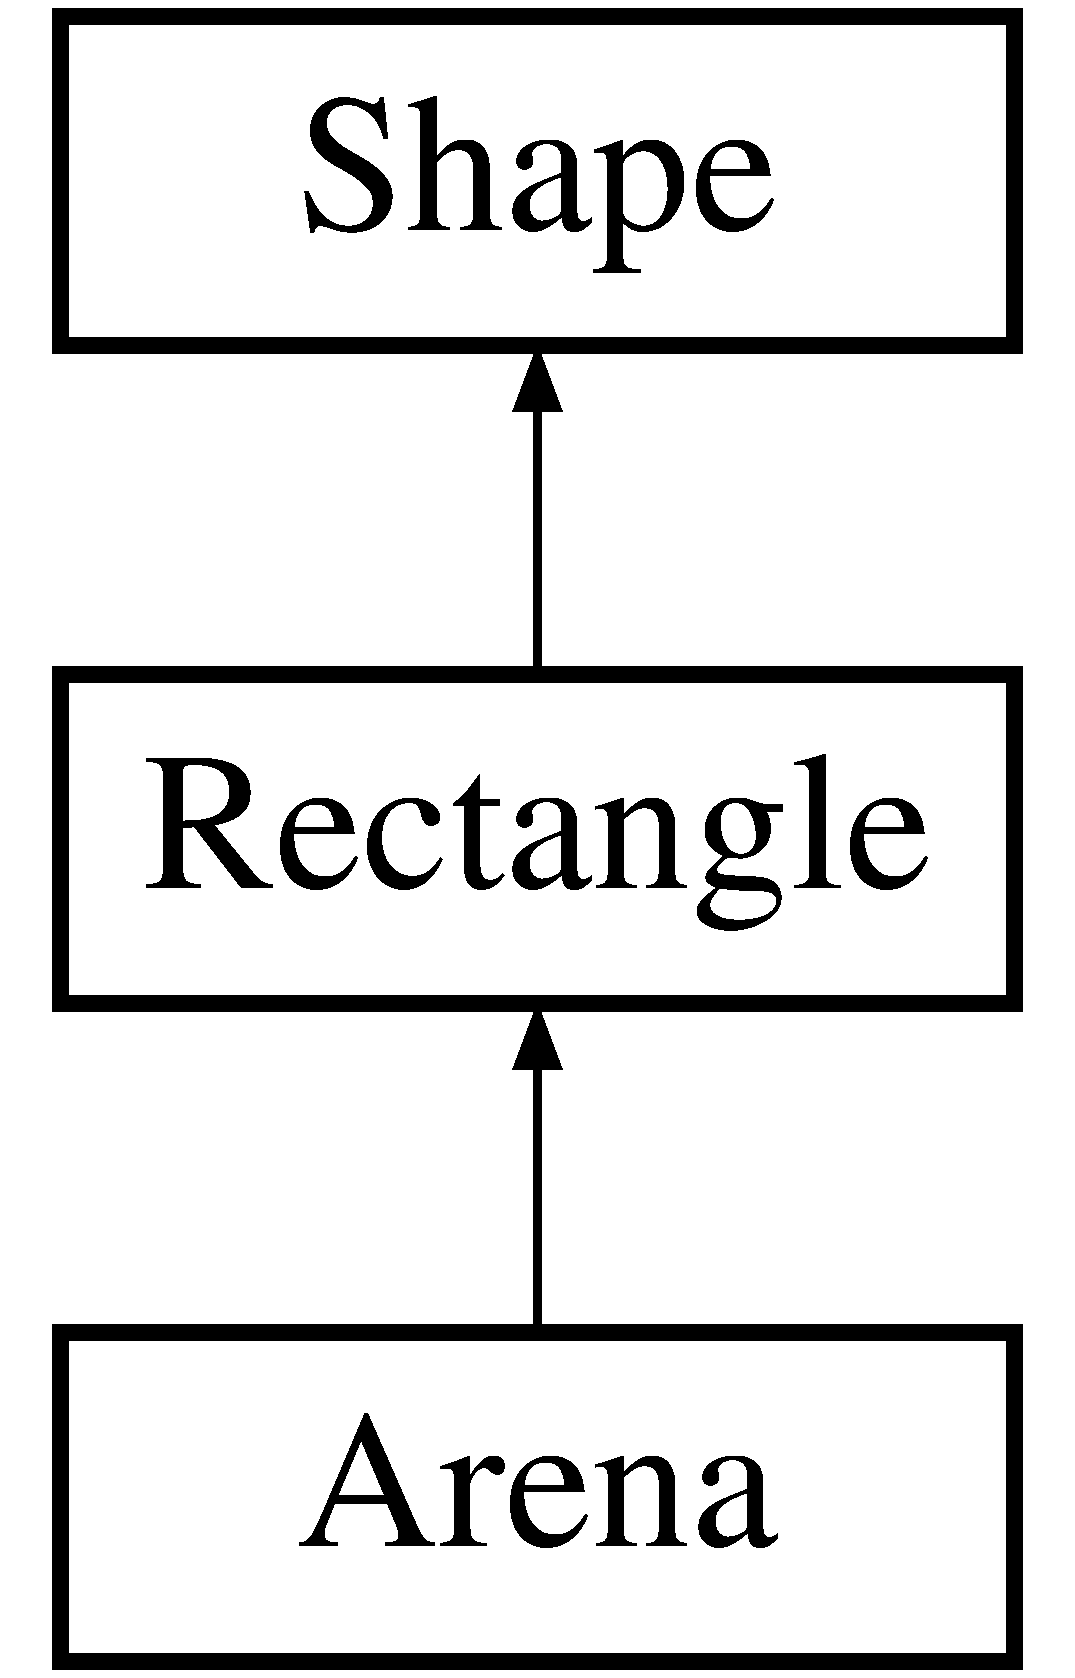
\includegraphics[height=2.000000cm]{class_arena}
\end{center}
\end{figure}
\subsection*{Public Member Functions}
\begin{DoxyCompactItemize}
\item 
\mbox{\Hypertarget{class_arena_aa37acdf43108ab0da04b77bbf79c2f7d}\label{class_arena_aa37acdf43108ab0da04b77bbf79c2f7d}} 
void {\bfseries find\+Arena} (const Mat \&img)
\item 
\mbox{\Hypertarget{class_arena_a67171d93c7aff0f9d8bd3ee0596e9033}\label{class_arena_a67171d93c7aff0f9d8bd3ee0596e9033}} 
std\+::vector$<$ cv\+::\+Point $>$ {\bfseries get\+Corners} ()
\item 
\mbox{\Hypertarget{class_arena_a7f822f33ff5810d4d266183e7606c0fe}\label{class_arena_a7f822f33ff5810d4d266183e7606c0fe}} 
void {\bfseries set\+Corners} (std\+::vector$<$ cv\+::\+Point $>$ corners)
\item 
\mbox{\Hypertarget{class_arena_ae7219e6d298213627a0c671e5c5f9536}\label{class_arena_ae7219e6d298213627a0c671e5c5f9536}} 
cv\+::\+Point {\bfseries get\+Top\+Left} ()
\item 
\mbox{\Hypertarget{class_arena_a7ab570cb7821df75c6da9af6491be034}\label{class_arena_a7ab570cb7821df75c6da9af6491be034}} 
void {\bfseries set\+Top\+Left} (cv\+::\+Point top\+Left)
\item 
\mbox{\Hypertarget{class_arena_aa417bc8757d66038038ac3f6a9d44860}\label{class_arena_aa417bc8757d66038038ac3f6a9d44860}} 
cv\+::\+Point {\bfseries get\+Top\+Right} ()
\item 
\mbox{\Hypertarget{class_arena_a82c7fa04e8acf52f6edecc1ee1c38001}\label{class_arena_a82c7fa04e8acf52f6edecc1ee1c38001}} 
void {\bfseries set\+Top\+Right} (cv\+::\+Point top\+Right)
\item 
\mbox{\Hypertarget{class_arena_afdd88e341c385561eafbc73e90e08404}\label{class_arena_afdd88e341c385561eafbc73e90e08404}} 
cv\+::\+Point {\bfseries get\+Bottom\+Left} ()
\item 
\mbox{\Hypertarget{class_arena_ac546db1983967fcc195369c8a0f1f9e5}\label{class_arena_ac546db1983967fcc195369c8a0f1f9e5}} 
void {\bfseries set\+Bottom\+Left} (cv\+::\+Point bottom\+Left)
\item 
\mbox{\Hypertarget{class_arena_ac62870a7bfa41baa7d38c4f7373cf3f5}\label{class_arena_ac62870a7bfa41baa7d38c4f7373cf3f5}} 
cv\+::\+Point {\bfseries get\+Bottom\+Right} ()
\item 
\mbox{\Hypertarget{class_arena_a2207ae5feab0d9ef8a19ab46fdd8685c}\label{class_arena_a2207ae5feab0d9ef8a19ab46fdd8685c}} 
void {\bfseries set\+Bottom\+Right} (cv\+::\+Point bottom\+Right)
\end{DoxyCompactItemize}


The documentation for this class was generated from the following file\+:\begin{DoxyCompactItemize}
\item 
Arena.\+hpp\end{DoxyCompactItemize}

\hypertarget{class_calibration___instrinsic}{}\section{Calibration\+\_\+\+Instrinsic Class Reference}
\label{class_calibration___instrinsic}\index{Calibration\+\_\+\+Instrinsic@{Calibration\+\_\+\+Instrinsic}}
\subsection*{Static Public Member Functions}
\begin{DoxyCompactItemize}
\item 
\mbox{\Hypertarget{class_calibration___instrinsic_a65d585bbfe48d2c1cedbc0f1b43b05d5}\label{class_calibration___instrinsic_a65d585bbfe48d2c1cedbc0f1b43b05d5}} 
static void {\bfseries perform\+Calibration} (const std\+::string cali\+\_\+config)
\item 
\mbox{\Hypertarget{class_calibration___instrinsic_aa8de03a03a709d52c9ac4e076e99072e}\label{class_calibration___instrinsic_aa8de03a03a709d52c9ac4e076e99072e}} 
static bool {\bfseries run\+Calibration\+And\+Save} (\mbox{\hyperlink{class_settings}{Settings}} \&s, Size image\+Size, Mat \&camera\+Matrix, Mat \&dist\+Coeffs, std\+::vector$<$ std\+::vector$<$ Point2f $>$ $>$ image\+Points)
\item 
\mbox{\Hypertarget{class_calibration___instrinsic_aec65e62022a78dd3c200ab613d4e1256}\label{class_calibration___instrinsic_aec65e62022a78dd3c200ab613d4e1256}} 
static bool {\bfseries run\+Calibration} (\mbox{\hyperlink{class_settings}{Settings}} \&s, Size \&image\+Size, Mat \&camera\+Matrix, Mat \&dist\+Coeffs, std\+::vector$<$ std\+::vector$<$ Point2f $>$ $>$ image\+Points, std\+::vector$<$ Mat $>$ \&rvecs, std\+::vector$<$ Mat $>$ \&tvecs, std\+::vector$<$ float $>$ \&reproj\+Errs, double \&total\+Avg\+Err)
\end{DoxyCompactItemize}


The documentation for this class was generated from the following file\+:\begin{DoxyCompactItemize}
\item 
Calibration\+\_\+\+Intrinsic.\+hpp\end{DoxyCompactItemize}

\hypertarget{class_cell}{}\section{Cell Class Reference}
\label{class_cell}\index{Cell@{Cell}}
\subsection*{Public Member Functions}
\begin{DoxyCompactItemize}
\item 
\mbox{\Hypertarget{class_cell_a03becce6b307d86848e9563eb08ac2b3}\label{class_cell_a03becce6b307d86848e9563eb08ac2b3}} 
std\+::vector$<$ cv\+::\+Point $>$ {\bfseries get\+Corners} ()
\item 
\mbox{\Hypertarget{class_cell_a6d1ad0f2766cdd641ba0e65f8b3c9555}\label{class_cell_a6d1ad0f2766cdd641ba0e65f8b3c9555}} 
void {\bfseries set\+Corners} (std\+::vector$<$ cv\+::\+Point $>$ corners)
\item 
\mbox{\Hypertarget{class_cell_ac6e9338748b2098e034641c88a977b23}\label{class_cell_ac6e9338748b2098e034641c88a977b23}} 
cv\+::\+Point {\bfseries get\+Top\+Left} ()
\item 
\mbox{\Hypertarget{class_cell_a9e2d13652a170ef25265a41dfe39e93f}\label{class_cell_a9e2d13652a170ef25265a41dfe39e93f}} 
void {\bfseries set\+Top\+Left} (cv\+::\+Point top\+Left)
\item 
\mbox{\Hypertarget{class_cell_a4b08bffc22a4393fd86c9608d9723d7c}\label{class_cell_a4b08bffc22a4393fd86c9608d9723d7c}} 
cv\+::\+Point {\bfseries get\+Top\+Right} ()
\item 
\mbox{\Hypertarget{class_cell_a245afe36e263e2fbf66880e4ea628f40}\label{class_cell_a245afe36e263e2fbf66880e4ea628f40}} 
void {\bfseries set\+Top\+Right} (cv\+::\+Point top\+Right)
\item 
\mbox{\Hypertarget{class_cell_a1946142c5e112176e1cd20cc6d07f831}\label{class_cell_a1946142c5e112176e1cd20cc6d07f831}} 
cv\+::\+Point {\bfseries get\+Bottom\+Left} ()
\item 
\mbox{\Hypertarget{class_cell_a86387a50a4c3f641eede253ce6cfcddb}\label{class_cell_a86387a50a4c3f641eede253ce6cfcddb}} 
void {\bfseries set\+Bottom\+Left} (cv\+::\+Point bottom\+Left)
\item 
\mbox{\Hypertarget{class_cell_afa1704102095fd55ac036f7d290eed05}\label{class_cell_afa1704102095fd55ac036f7d290eed05}} 
cv\+::\+Point {\bfseries get\+Bottom\+Right} ()
\item 
\mbox{\Hypertarget{class_cell_ae68ff90cfde34cec208e8e74ce3f2745}\label{class_cell_ae68ff90cfde34cec208e8e74ce3f2745}} 
void {\bfseries set\+Bottom\+Right} (cv\+::\+Point bottom\+Right)
\item 
\mbox{\Hypertarget{class_cell_a6c7344ef2aa917e70364221bf86ff8bc}\label{class_cell_a6c7344ef2aa917e70364221bf86ff8bc}} 
bool {\bfseries is\+Empty} ()
\item 
\mbox{\Hypertarget{class_cell_aaf13f5d308c7f1eb670a050e4fc6dc28}\label{class_cell_aaf13f5d308c7f1eb670a050e4fc6dc28}} 
bool {\bfseries is\+Exit} ()
\item 
\mbox{\Hypertarget{class_cell_a34d62b7c65fd85f356bd9e2c3058edcb}\label{class_cell_a34d62b7c65fd85f356bd9e2c3058edcb}} 
bool {\bfseries is\+Border} ()
\item 
\mbox{\Hypertarget{class_cell_aee32093f779b1fa761b43a6b0a86ed6c}\label{class_cell_aee32093f779b1fa761b43a6b0a86ed6c}} 
bool {\bfseries is\+Obstacle} ()
\item 
\mbox{\Hypertarget{class_cell_ad86a719c04ff04bdf79c1c0b8e5a5942}\label{class_cell_ad86a719c04ff04bdf79c1c0b8e5a5942}} 
bool {\bfseries is\+Rescue} ()
\item 
\mbox{\Hypertarget{class_cell_a335c410074aaac9bb5594ea8adf648ff}\label{class_cell_a335c410074aaac9bb5594ea8adf648ff}} 
int {\bfseries get\+Digit} ()
\item 
\mbox{\Hypertarget{class_cell_a6047939b792e819bc2330151ff98864f}\label{class_cell_a6047939b792e819bc2330151ff98864f}} 
void {\bfseries set\+Empty} ()
\item 
\mbox{\Hypertarget{class_cell_a9fa0a3c17d798320c78bffe44411008e}\label{class_cell_a9fa0a3c17d798320c78bffe44411008e}} 
void {\bfseries set\+Exit} ()
\item 
\mbox{\Hypertarget{class_cell_aa690e62809d36d512cd39ccda9cea293}\label{class_cell_aa690e62809d36d512cd39ccda9cea293}} 
void {\bfseries set\+Border} ()
\item 
\mbox{\Hypertarget{class_cell_a34e953e7f720c3382f0b13c2480cafd0}\label{class_cell_a34e953e7f720c3382f0b13c2480cafd0}} 
void {\bfseries set\+Obstacle} ()
\item 
\mbox{\Hypertarget{class_cell_afa194cda3c1e8f9be100c9a14fda7f9d}\label{class_cell_afa194cda3c1e8f9be100c9a14fda7f9d}} 
void {\bfseries set\+Rescue} (int digit\+\_\+i)
\end{DoxyCompactItemize}


The documentation for this class was generated from the following file\+:\begin{DoxyCompactItemize}
\item 
Cell.\+hpp\end{DoxyCompactItemize}

\hypertarget{class_character___recognition___algorithm}{}\section{Character\+\_\+\+Recognition\+\_\+\+Algorithm Class Reference}
\label{class_character___recognition___algorithm}\index{Character\+\_\+\+Recognition\+\_\+\+Algorithm@{Character\+\_\+\+Recognition\+\_\+\+Algorithm}}


abstract class for character recognition algorithms  




{\ttfamily \#include $<$Character\+\_\+\+Recognition\+\_\+\+Algorithm.\+hpp$>$}

Inheritance diagram for Character\+\_\+\+Recognition\+\_\+\+Algorithm\+:\begin{figure}[H]
\begin{center}
\leavevmode
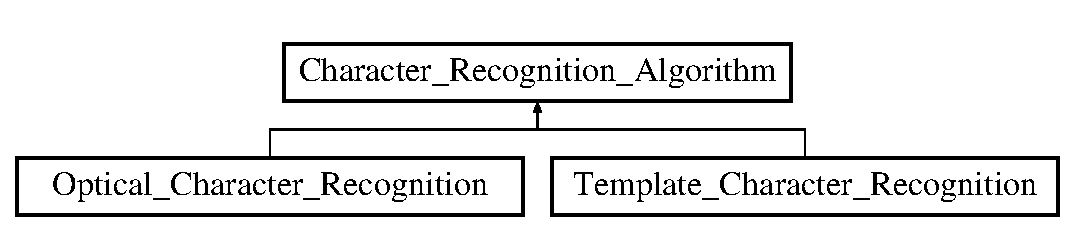
\includegraphics[height=2.000000cm]{class_character___recognition___algorithm}
\end{center}
\end{figure}
\subsection*{Public Member Functions}
\begin{DoxyCompactItemize}
\item 
\mbox{\Hypertarget{class_character___recognition___algorithm_ae830baa9ccf7c55ad73c78173188059e}\label{class_character___recognition___algorithm_ae830baa9ccf7c55ad73c78173188059e}} 
virtual void \mbox{\hyperlink{class_character___recognition___algorithm_ae830baa9ccf7c55ad73c78173188059e}{process\+Image}} (const std\+::string \&filename)=0
\begin{DoxyCompactList}\small\item\em a demo function displaying the performance of a given algorithm \end{DoxyCompactList}\item 
\mbox{\Hypertarget{class_character___recognition___algorithm_ad360b10ac65fe20b42607ef9568052a3}\label{class_character___recognition___algorithm_ad360b10ac65fe20b42607ef9568052a3}} 
virtual int \mbox{\hyperlink{class_character___recognition___algorithm_ad360b10ac65fe20b42607ef9568052a3}{detect\+\_\+digit}} (cv\+::\+Mat \&image, cv\+::\+Rect \&rect, cv\+::\+Mat \&R\+OI)=0
\begin{DoxyCompactList}\small\item\em the (virtual) function that runs the recognition engine \end{DoxyCompactList}\item 
\mbox{\Hypertarget{class_character___recognition___algorithm_af17cbb0e6b84fd9430ff1788f6c57740}\label{class_character___recognition___algorithm_af17cbb0e6b84fd9430ff1788f6c57740}} 
virtual std\+::vector$<$ std\+::pair$<$ int, cv\+::\+Rect $>$ $>$ {\bfseries detection\+\_\+algorithm} (std\+::vector$<$ cv\+::\+Rect $>$ \&bound\+Rect, cv\+::\+Mat \&filtered)=0
\item 
\mbox{\Hypertarget{class_character___recognition___algorithm_ae6fbf353044a0d3d1c4703bff3a46080}\label{class_character___recognition___algorithm_ae6fbf353044a0d3d1c4703bff3a46080}} 
void {\bfseries display\+Image} (cv\+::\+Mat \&image, std\+::string window\+Title)
\item 
\mbox{\Hypertarget{class_character___recognition___algorithm_ad7302516bfe29b94dd6787cfb4aa9183}\label{class_character___recognition___algorithm_ad7302516bfe29b94dd6787cfb4aa9183}} 
cv\+::\+Mat {\bfseries load\+Image} (const std\+::string \&filename)
\item 
\mbox{\Hypertarget{class_character___recognition___algorithm_ab393524887755e6e363d281856b8aa1e}\label{class_character___recognition___algorithm_ab393524887755e6e363d281856b8aa1e}} 
void {\bfseries convert\+\_\+bgr\+\_\+to\+\_\+hsv} (cv\+::\+Mat \&original, cv\+::\+Mat \&converted)
\item 
\mbox{\Hypertarget{class_character___recognition___algorithm_af84b6a4dad5edcf27f65d5dbc884efb2}\label{class_character___recognition___algorithm_af84b6a4dad5edcf27f65d5dbc884efb2}} 
void {\bfseries apply\+\_\+mask} (cv\+::\+Mat \&original, cv\+::\+Mat \&converted, cv\+::\+Scalar lowerbound, cv\+::\+Scalar upperbound)
\item 
\mbox{\Hypertarget{class_character___recognition___algorithm_a5f8eaa507a9b61ba71d361e2306d0110}\label{class_character___recognition___algorithm_a5f8eaa507a9b61ba71d361e2306d0110}} 
cv\+::\+Mat {\bfseries apply\+\_\+some\+\_\+filtering} (cv\+::\+Mat \&img)
\item 
\mbox{\Hypertarget{class_character___recognition___algorithm_a21924694ba0aacb82054ea33191cb52a}\label{class_character___recognition___algorithm_a21924694ba0aacb82054ea33191cb52a}} 
std\+::vector$<$ cv\+::\+Rect $>$ {\bfseries extract\+\_\+regions\+\_\+of\+\_\+interest} (cv\+::\+Mat \&original\+\_\+img, cv\+::\+Mat \&filtered\+\_\+img, cv\+::\+Mat \&returned\+Img)
\item 
\mbox{\Hypertarget{class_character___recognition___algorithm_a75ff23b5b2722c9c572091755985e137}\label{class_character___recognition___algorithm_a75ff23b5b2722c9c572091755985e137}} 
std\+::tuple$<$ cv\+::\+Mat, cv\+::\+Mat $>$ {\bfseries invert\+\_\+masked\+\_\+image} (cv\+::\+Mat \&original, cv\+::\+Mat \&masked\+\_\+image)
\item 
\mbox{\Hypertarget{class_character___recognition___algorithm_a4f7714bd67ad5804c909859b8eb5b8c6}\label{class_character___recognition___algorithm_a4f7714bd67ad5804c909859b8eb5b8c6}} 
void {\bfseries rotate\+\_\+image} (cv\+::\+Mat \&src, double angle, cv\+::\+Mat \&result)
\item 
\mbox{\Hypertarget{class_character___recognition___algorithm_a7642ccec81710fa52c553c13dcf7e0ca}\label{class_character___recognition___algorithm_a7642ccec81710fa52c553c13dcf7e0ca}} 
void {\bfseries preprocessing} (cv\+::\+Mat \&img, cv\+::\+Mat \&filtered, std\+::vector$<$ cv\+::\+Rect $>$ \&bound\+Rect)
\item 
\mbox{\Hypertarget{class_character___recognition___algorithm_a06c2a31ba8f4ab6e3aacea6b643a4d7d}\label{class_character___recognition___algorithm_a06c2a31ba8f4ab6e3aacea6b643a4d7d}} 
void {\bfseries set\+\_\+lower\+\_\+bound\+\_\+filter} (double hue, double saturation, double value)
\item 
\mbox{\Hypertarget{class_character___recognition___algorithm_a2add4eeeb34fb3a8bd35a1d5da0950a0}\label{class_character___recognition___algorithm_a2add4eeeb34fb3a8bd35a1d5da0950a0}} 
void {\bfseries set\+\_\+upper\+\_\+bound\+\_\+filter} (double hue, double saturation, double value)
\end{DoxyCompactItemize}
\subsection*{Public Attributes}
\begin{DoxyCompactItemize}
\item 
\mbox{\Hypertarget{class_character___recognition___algorithm_a6fda22815d819ef7d0b0cfec4baba47c}\label{class_character___recognition___algorithm_a6fda22815d819ef7d0b0cfec4baba47c}} 
const double {\bfseries M\+I\+N\+\_\+\+A\+R\+E\+A\+\_\+\+S\+I\+ZE} = 100
\item 
\mbox{\Hypertarget{class_character___recognition___algorithm_a3792c162037a2049d991a1634576d915}\label{class_character___recognition___algorithm_a3792c162037a2049d991a1634576d915}} 
\mbox{\hyperlink{struct_h_s_v_filter_range}{H\+S\+V\+Filter\+Range}} {\bfseries filter} = \mbox{\hyperlink{struct_h_s_v_filter_range}{H\+S\+V\+Filter\+Range}}()
\item 
\mbox{\Hypertarget{class_character___recognition___algorithm_a9c22f95223ecc5cfaf8e0303c30d5379}\label{class_character___recognition___algorithm_a9c22f95223ecc5cfaf8e0303c30d5379}} 
double {\bfseries delta\+\_\+angle} = 45
\end{DoxyCompactItemize}


\subsection{Detailed Description}
abstract class for character recognition algorithms 

The documentation for this class was generated from the following file\+:\begin{DoxyCompactItemize}
\item 
Character\+\_\+\+Recognition\+\_\+\+Algorithm.\+hpp\end{DoxyCompactItemize}

\hypertarget{class_circle}{}\section{Circle Class Reference}
\label{class_circle}\index{Circle@{Circle}}
Inheritance diagram for Circle\+:\begin{figure}[H]
\begin{center}
\leavevmode
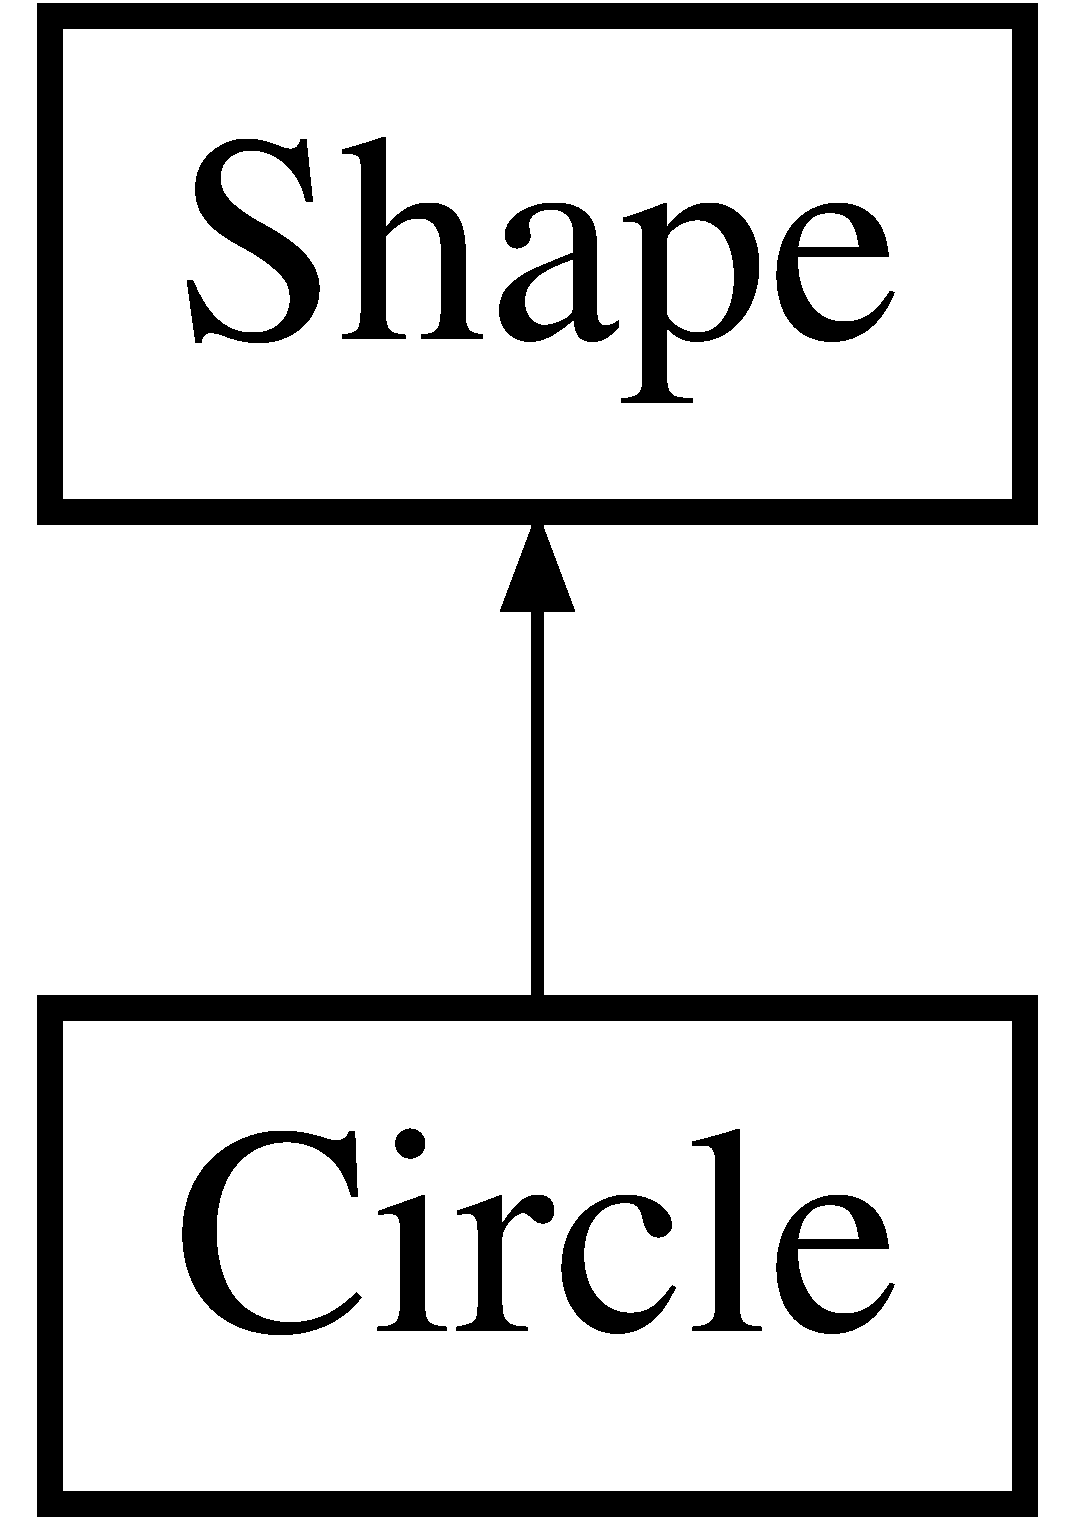
\includegraphics[height=2.000000cm]{class_circle}
\end{center}
\end{figure}
\subsection*{Public Member Functions}
\begin{DoxyCompactItemize}
\item 
\mbox{\Hypertarget{class_circle_adfc2e5e026f5d80215563cc42260a237}\label{class_circle_adfc2e5e026f5d80215563cc42260a237}} 
int {\bfseries get\+Radius} ()
\item 
\mbox{\Hypertarget{class_circle_ae4a8bd93b437b4cf0077483ff84c8626}\label{class_circle_ae4a8bd93b437b4cf0077483ff84c8626}} 
void {\bfseries set\+Radius} (int radius\+\_\+c)
\item 
\mbox{\Hypertarget{class_circle_a60d1af499a6ad295f9f2955c4409dddd}\label{class_circle_a60d1af499a6ad295f9f2955c4409dddd}} 
cv\+::\+Point {\bfseries get\+Center} ()
\item 
\mbox{\Hypertarget{class_circle_a242599150a3623ea837fcb599214e33b}\label{class_circle_a242599150a3623ea837fcb599214e33b}} 
void {\bfseries set\+Center} (cv\+::\+Point center\+\_\+c)
\item 
\mbox{\Hypertarget{class_circle_a50656c826a70e13fa75eb696a0dd3123}\label{class_circle_a50656c826a70e13fa75eb696a0dd3123}} 
int {\bfseries get\+Digit} ()
\item 
\mbox{\Hypertarget{class_circle_a187d5c4d66124603abb89f57552b6c4c}\label{class_circle_a187d5c4d66124603abb89f57552b6c4c}} 
void {\bfseries set\+Digit} (int digit\+\_\+i)
\end{DoxyCompactItemize}


The documentation for this class was generated from the following file\+:\begin{DoxyCompactItemize}
\item 
Circle.\+hpp\end{DoxyCompactItemize}

\hypertarget{class_circular_line}{}\section{Circular\+Line Class Reference}
\label{class_circular_line}\index{Circular\+Line@{Circular\+Line}}


Class for managing circle in the pat.  




{\ttfamily \#include $<$Circular\+Line.\+hpp$>$}

Inheritance diagram for Circular\+Line\+:\begin{figure}[H]
\begin{center}
\leavevmode
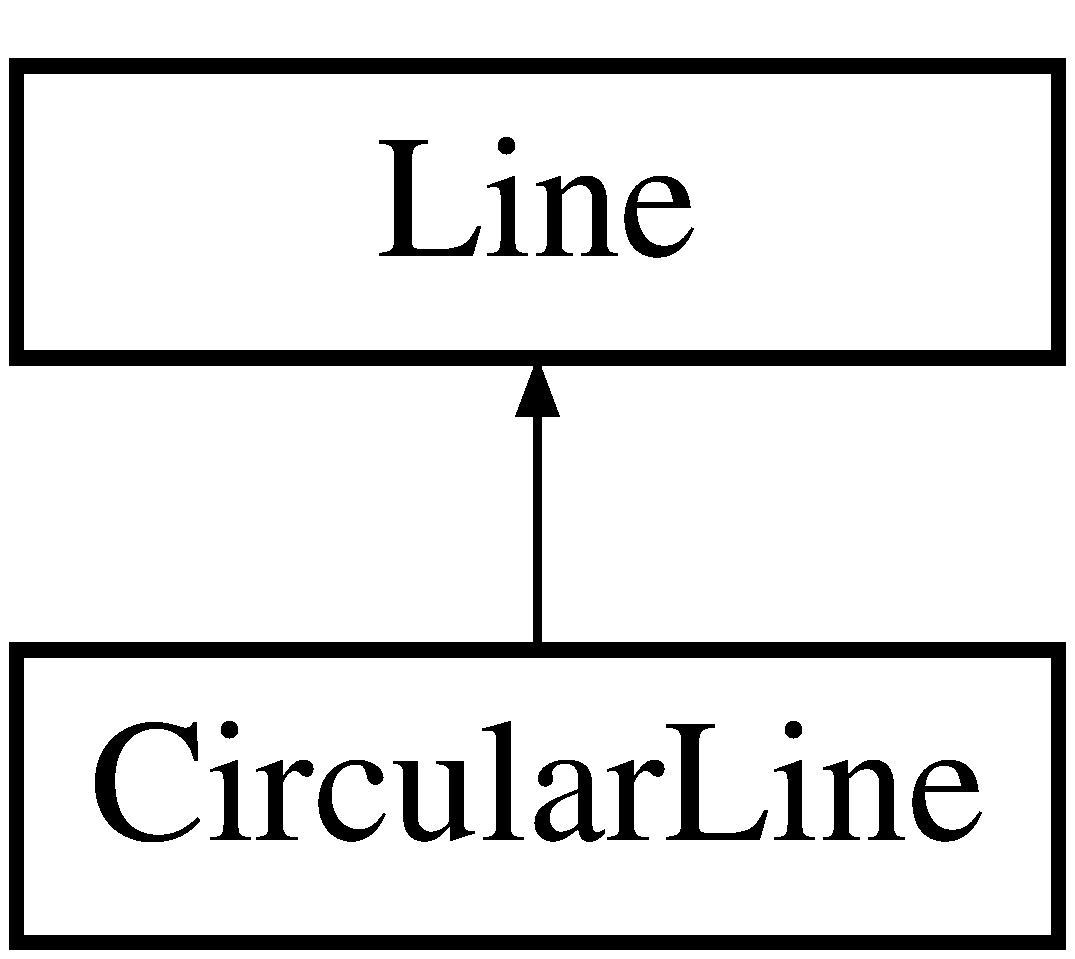
\includegraphics[height=2.000000cm]{class_circular_line}
\end{center}
\end{figure}
\subsection*{Public Member Functions}
\begin{DoxyCompactItemize}
\item 
\mbox{\hyperlink{class_circular_line_aacb17f31ed3eb9fbe66fbe2a95b20e6a}{Circular\+Line}} (\mbox{\hyperlink{class_position}{Position}} start\+\_\+point, double curvature, double length)
\begin{DoxyCompactList}\small\item\em constructor of the class \end{DoxyCompactList}\item 
\mbox{\Hypertarget{class_circular_line_a2f8c59281cb51a6072b6980b6df9be89}\label{class_circular_line_a2f8c59281cb51a6072b6980b6df9be89}} 
\mbox{\hyperlink{class_circular_line_a2f8c59281cb51a6072b6980b6df9be89}{$\sim$\+Circular\+Line}} ()
\begin{DoxyCompactList}\small\item\em destructor of the class \end{DoxyCompactList}\item 
\mbox{\Hypertarget{class_circular_line_a521ac7d10eca4ea8914465c5eea90d8d}\label{class_circular_line_a521ac7d10eca4ea8914465c5eea90d8d}} 
void \mbox{\hyperlink{class_circular_line_a521ac7d10eca4ea8914465c5eea90d8d}{set\+Curvature}} (double curvature\+\_\+i)
\begin{DoxyCompactList}\small\item\em allow to set the curvature of the line \end{DoxyCompactList}\item 
double \mbox{\hyperlink{class_circular_line_ab5bad8246cee1a80c1e625c68c0b2c15}{get\+Curvature}} ()
\end{DoxyCompactItemize}


\subsection{Detailed Description}
Class for managing circle in the pat. 

\subsection{Constructor \& Destructor Documentation}
\mbox{\Hypertarget{class_circular_line_aacb17f31ed3eb9fbe66fbe2a95b20e6a}\label{class_circular_line_aacb17f31ed3eb9fbe66fbe2a95b20e6a}} 
\index{Circular\+Line@{Circular\+Line}!Circular\+Line@{Circular\+Line}}
\index{Circular\+Line@{Circular\+Line}!Circular\+Line@{Circular\+Line}}
\subsubsection{\texorpdfstring{Circular\+Line()}{CircularLine()}}
{\footnotesize\ttfamily Circular\+Line\+::\+Circular\+Line (\begin{DoxyParamCaption}\item[{\mbox{\hyperlink{class_position}{Position}}}]{start\+\_\+point,  }\item[{double}]{curvature,  }\item[{double}]{length }\end{DoxyParamCaption})}



constructor of the class 


\begin{DoxyParams}{Parameters}
{\em start\+\_\+point} & start position of the line \\
\hline
{\em curvature} & curvature of the path \\
\hline
{\em length} & length of the path \\
\hline
\end{DoxyParams}


\subsection{Member Function Documentation}
\mbox{\Hypertarget{class_circular_line_ab5bad8246cee1a80c1e625c68c0b2c15}\label{class_circular_line_ab5bad8246cee1a80c1e625c68c0b2c15}} 
\index{Circular\+Line@{Circular\+Line}!get\+Curvature@{get\+Curvature}}
\index{get\+Curvature@{get\+Curvature}!Circular\+Line@{Circular\+Line}}
\subsubsection{\texorpdfstring{get\+Curvature()}{getCurvature()}}
{\footnotesize\ttfamily double Circular\+Line\+::get\+Curvature (\begin{DoxyParamCaption}{ }\end{DoxyParamCaption})}

return the curvature of the line \begin{DoxyReturn}{Returns}
curvature of the line 
\end{DoxyReturn}


The documentation for this class was generated from the following file\+:\begin{DoxyCompactItemize}
\item 
Circular\+Line.\+hpp\end{DoxyCompactItemize}

\hypertarget{class_collision_detector}{}\section{Collision\+Detector Class Reference}
\label{class_collision_detector}\index{Collision\+Detector@{Collision\+Detector}}


detector of collision between obstacles and path  




{\ttfamily \#include $<$Collision\+Detector.\+hpp$>$}

\subsection*{Public Member Functions}
\begin{DoxyCompactItemize}
\item 
\mbox{\Hypertarget{class_collision_detector_ab3f66bd8d272a21674e38bf46d4d31e0}\label{class_collision_detector_ab3f66bd8d272a21674e38bf46d4d31e0}} 
\mbox{\hyperlink{class_collision_detector_ab3f66bd8d272a21674e38bf46d4d31e0}{Collision\+Detector}} ()
\begin{DoxyCompactList}\small\item\em constructor of Collision\+Detector\+\_\+hpp class \end{DoxyCompactList}\item 
\mbox{\Hypertarget{class_collision_detector_a1a0f7a386920e0cf83a101be92f04598}\label{class_collision_detector_a1a0f7a386920e0cf83a101be92f04598}} 
\mbox{\hyperlink{class_collision_detector_a1a0f7a386920e0cf83a101be92f04598}{$\sim$\+Collision\+Detector}} ()
\begin{DoxyCompactList}\small\item\em destructor of Collision\+Detector\+\_\+hpp class \end{DoxyCompactList}\item 
bool \mbox{\hyperlink{class_collision_detector_a190378f3f5714c8c75e5e5baabcfe2e7}{detect\+Collision}} (std\+::vector$<$ \mbox{\hyperlink{class_line}{Line}} $>$ lines\+\_\+i, \mbox{\hyperlink{class_map}{Map}} $\ast$map, double max\+\_\+curvature)
\begin{DoxyCompactList}\small\item\em given a vector of lines detect if the path is feasible \end{DoxyCompactList}\end{DoxyCompactItemize}


\subsection{Detailed Description}
detector of collision between obstacles and path 

\subsection{Member Function Documentation}
\mbox{\Hypertarget{class_collision_detector_a190378f3f5714c8c75e5e5baabcfe2e7}\label{class_collision_detector_a190378f3f5714c8c75e5e5baabcfe2e7}} 
\index{Collision\+Detector@{Collision\+Detector}!detect\+Collision@{detect\+Collision}}
\index{detect\+Collision@{detect\+Collision}!Collision\+Detector@{Collision\+Detector}}
\subsubsection{\texorpdfstring{detect\+Collision()}{detectCollision()}}
{\footnotesize\ttfamily bool Collision\+Detector\+::detect\+Collision (\begin{DoxyParamCaption}\item[{std\+::vector$<$ \mbox{\hyperlink{class_line}{Line}} $>$}]{lines\+\_\+i,  }\item[{\mbox{\hyperlink{class_map}{Map}} $\ast$}]{map,  }\item[{double}]{max\+\_\+curvature }\end{DoxyParamCaption})}



given a vector of lines detect if the path is feasible 


\begin{DoxyParams}{Parameters}
{\em lines\+\_\+i} & vector of line that we want to check \\
\hline
{\em map} & map of the arena \\
\hline
{\em max\+\_\+curvature} & curvature of the path \\
\hline
\end{DoxyParams}
\begin{DoxyReturn}{Returns}
true if there is a collision false otherwise 
\end{DoxyReturn}


The documentation for this class was generated from the following file\+:\begin{DoxyCompactItemize}
\item 
Collision\+Detector.\+hpp\end{DoxyCompactItemize}

\hypertarget{class_color___processing}{}\section{Color\+\_\+\+Processing Class Reference}
\label{class_color___processing}\index{Color\+\_\+\+Processing@{Color\+\_\+\+Processing}}
\subsection*{Public Member Functions}
\begin{DoxyCompactItemize}
\item 
\mbox{\Hypertarget{class_color___processing_a293f699a508b29f6a040f80363b5175c}\label{class_color___processing_a293f699a508b29f6a040f80363b5175c}} 
void {\bfseries load\+\_\+pixels} (cv\+::\+Mat \&img)
\item 
\mbox{\Hypertarget{class_color___processing_a1b6c44ee9495d9d453545b57640be8cd}\label{class_color___processing_a1b6c44ee9495d9d453545b57640be8cd}} 
\mbox{\hyperlink{struct_h_s_v_filter_range}{H\+S\+V\+Filter\+Range}} {\bfseries get\+Filter} ()
\item 
\mbox{\Hypertarget{class_color___processing_aff93a009843ca7762732984ef57375b9}\label{class_color___processing_aff93a009843ca7762732984ef57375b9}} 
void {\bfseries find\+\_\+black\+\_\+threshold} (cv\+::\+Mat \&img)
\item 
\mbox{\Hypertarget{class_color___processing_acb962976dba3538eabcf5812951a023e}\label{class_color___processing_acb962976dba3538eabcf5812951a023e}} 
void {\bfseries calibrate\+\_\+color} (const std\+::string filename)
\item 
\mbox{\Hypertarget{class_color___processing_aa5007ebc7ce0250d5028ee718bace4d4}\label{class_color___processing_aa5007ebc7ce0250d5028ee718bace4d4}} 
void {\bfseries demo} (cv\+::\+Mat \&img)
\end{DoxyCompactItemize}
\subsection*{Public Attributes}
\begin{DoxyCompactItemize}
\item 
\mbox{\Hypertarget{class_color___processing_a5769c226ab5a68929b0b5894d35dbb57}\label{class_color___processing_a5769c226ab5a68929b0b5894d35dbb57}} 
std\+::pair$<$ double, double $>$ {\bfseries range} = std\+::pair$<$double,double$>$ (0,0)
\item 
\mbox{\Hypertarget{class_color___processing_a46734d34d9efc70a1e15dcece2a2336e}\label{class_color___processing_a46734d34d9efc70a1e15dcece2a2336e}} 
std\+::pair$<$ double, double $>$ {\bfseries black\+\_\+threshold} = std\+::pair$<$double,double$>$ (0,0)
\item 
\mbox{\Hypertarget{class_color___processing_a8702c050fe8071a91a3d4376b76ac0d5}\label{class_color___processing_a8702c050fe8071a91a3d4376b76ac0d5}} 
std\+::vector$<$ cv\+::\+Vec3b $>$ {\bfseries pixels}
\end{DoxyCompactItemize}


The documentation for this class was generated from the following file\+:\begin{DoxyCompactItemize}
\item 
Color\+\_\+\+Processing.\+hpp\end{DoxyCompactItemize}

\hypertarget{class_digit___recognition}{}\section{Digit\+\_\+\+Recognition Class Reference}
\label{class_digit___recognition}\index{Digit\+\_\+\+Recognition@{Digit\+\_\+\+Recognition}}


The \mbox{\hyperlink{class_digit___recognition}{Digit\+\_\+\+Recognition}} class is used to detect digits in the arena and export \mbox{\hyperlink{struct_people_data}{People\+Data}}.  




{\ttfamily \#include $<$Digit\+\_\+\+Recognition.\+hpp$>$}

\subsection*{Public Member Functions}
\begin{DoxyCompactItemize}
\item 
\mbox{\hyperlink{class_digit___recognition_a183d686f4f9f3ce1ed555e9311d30f56}{Digit\+\_\+\+Recognition}} (Digit\+Recognition\+Algo algorithm)
\begin{DoxyCompactList}\small\item\em constructing the class with a set Digit\+Recognition\+Algo type \end{DoxyCompactList}\item 
\mbox{\Hypertarget{class_digit___recognition_a5c83d879c6881693c3606cc5a1bc8ef2}\label{class_digit___recognition_a5c83d879c6881693c3606cc5a1bc8ef2}} 
void \mbox{\hyperlink{class_digit___recognition_a5c83d879c6881693c3606cc5a1bc8ef2}{set\+\_\+algo}} (Digit\+Recognition\+Algo algorithm)
\begin{DoxyCompactList}\small\item\em set detection algorithm for digits e.\+g. tesseract or template matching \end{DoxyCompactList}\item 
\mbox{\Hypertarget{class_digit___recognition_a479e6126291463d9117abc6553c555df}\label{class_digit___recognition_a479e6126291463d9117abc6553c555df}} 
int \mbox{\hyperlink{class_digit___recognition_a479e6126291463d9117abc6553c555df}{detect\+\_\+digit\+\_\+for\+\_\+map}} (cv\+::\+Mat \&img)
\begin{DoxyCompactList}\small\item\em detects digit of prepared image and checks if the result was fitting the map requierements \end{DoxyCompactList}\item 
\mbox{\Hypertarget{class_digit___recognition_aad1207aa02e043af5505c217ef1996b9}\label{class_digit___recognition_aad1207aa02e043af5505c217ef1996b9}} 
std\+::vector$<$ \mbox{\hyperlink{struct_people_data}{People\+Data}} $>$ \mbox{\hyperlink{class_digit___recognition_aad1207aa02e043af5505c217ef1996b9}{detect\+\_\+digits\+\_\+for\+\_\+map}} (const cv\+::\+Mat img\+\_\+input)
\begin{DoxyCompactList}\small\item\em detects all the digits of an unprepared images and returns people information \end{DoxyCompactList}\item 
void \mbox{\hyperlink{class_digit___recognition_a68484f6730ee2f0fc2050726c3ff2252}{set\+\_\+filter}} (\mbox{\hyperlink{struct_h_s_v_filter_range}{H\+S\+V\+Filter\+Range}} filter\+Range)
\begin{DoxyCompactList}\small\item\em sets a hsv filter for better image recognition results \end{DoxyCompactList}\item 
std\+::vector$<$ cv\+::\+Rect $>$ \mbox{\hyperlink{class_digit___recognition_acb87e2fb3a72d625170ab8c95ef6828f}{get\+\_\+regions\+\_\+of\+\_\+interest}} (cv\+::\+Mat \&img)
\begin{DoxyCompactList}\small\item\em extracts the rect information of regions where the filter was applied \end{DoxyCompactList}\end{DoxyCompactItemize}
\subsection*{Public Attributes}
\begin{DoxyCompactItemize}
\item 
\mbox{\Hypertarget{class_digit___recognition_aae57bd40fa8864ed5085beb98aa22fcd}\label{class_digit___recognition_aae57bd40fa8864ed5085beb98aa22fcd}} 
Digit\+Recognition\+Algo \mbox{\hyperlink{class_digit___recognition_aae57bd40fa8864ed5085beb98aa22fcd}{picked\+\_\+algorithm}}
\begin{DoxyCompactList}\small\item\em the algorithm typed used to detect digits \end{DoxyCompactList}\end{DoxyCompactItemize}


\subsection{Detailed Description}
The \mbox{\hyperlink{class_digit___recognition}{Digit\+\_\+\+Recognition}} class is used to detect digits in the arena and export \mbox{\hyperlink{struct_people_data}{People\+Data}}. 

The \mbox{\hyperlink{class_digit___recognition}{Digit\+\_\+\+Recognition}} class is used to detect digits in the arena and export \mbox{\hyperlink{struct_people_data}{People\+Data}}. The class contains a \mbox{\hyperlink{class_character___recognition___algorithm}{Character\+\_\+\+Recognition\+\_\+\+Algorithm}} member that is used to detect digits. Changing the Digit\+Recognition\+Algo type results in the use of another implementation of \mbox{\hyperlink{class_character___recognition___algorithm}{Character\+\_\+\+Recognition\+\_\+\+Algorithm}} derived classes. New types of \mbox{\hyperlink{class_character___recognition___algorithm}{Character\+\_\+\+Recognition\+\_\+\+Algorithm}} subclasses can be added to improve digit recognition performance over time. The class contains \mbox{\hyperlink{struct_h_s_v_filter_range}{H\+S\+V\+Filter\+Range}} object that is able to automatically construct a color filter from a given input image. When detect\+\_\+digit\+\_\+for\+\_\+map is called the class will identify circles, use the filter to extract the digits, perform the digit recognition and export a \mbox{\hyperlink{struct_people_data}{People\+Data}} object that can be used to create \mbox{\hyperlink{class_people}{People}} objects and feed the map. \begin{DoxySeeAlso}{See also}
\mbox{\hyperlink{class_people}{People}} 

\mbox{\hyperlink{class_map}{Map}} 
\end{DoxySeeAlso}


\subsection{Constructor \& Destructor Documentation}
\mbox{\Hypertarget{class_digit___recognition_a183d686f4f9f3ce1ed555e9311d30f56}\label{class_digit___recognition_a183d686f4f9f3ce1ed555e9311d30f56}} 
\index{Digit\+\_\+\+Recognition@{Digit\+\_\+\+Recognition}!Digit\+\_\+\+Recognition@{Digit\+\_\+\+Recognition}}
\index{Digit\+\_\+\+Recognition@{Digit\+\_\+\+Recognition}!Digit\+\_\+\+Recognition@{Digit\+\_\+\+Recognition}}
\subsubsection{\texorpdfstring{Digit\+\_\+\+Recognition()}{Digit\_Recognition()}}
{\footnotesize\ttfamily Digit\+\_\+\+Recognition\+::\+Digit\+\_\+\+Recognition (\begin{DoxyParamCaption}\item[{Digit\+Recognition\+Algo}]{algorithm }\end{DoxyParamCaption})}



constructing the class with a set Digit\+Recognition\+Algo type 


\begin{DoxyParams}{Parameters}
{\em algorithm} & a Digit\+Recognition\+Algo enum type that specifies the type of \mbox{\hyperlink{class_character___recognition___algorithm}{Character\+\_\+\+Recognition\+\_\+\+Algorithm}} used to perform the recognition of the digit \\
\hline
\end{DoxyParams}
\begin{DoxySeeAlso}{See also}
Optical\+\_\+\+Recognition\+\_\+\+Algorithm, \mbox{\hyperlink{class_template___character___recognition}{Template\+\_\+\+Character\+\_\+\+Recognition}} 
\end{DoxySeeAlso}


\subsection{Member Function Documentation}
\mbox{\Hypertarget{class_digit___recognition_acb87e2fb3a72d625170ab8c95ef6828f}\label{class_digit___recognition_acb87e2fb3a72d625170ab8c95ef6828f}} 
\index{Digit\+\_\+\+Recognition@{Digit\+\_\+\+Recognition}!get\+\_\+regions\+\_\+of\+\_\+interest@{get\+\_\+regions\+\_\+of\+\_\+interest}}
\index{get\+\_\+regions\+\_\+of\+\_\+interest@{get\+\_\+regions\+\_\+of\+\_\+interest}!Digit\+\_\+\+Recognition@{Digit\+\_\+\+Recognition}}
\subsubsection{\texorpdfstring{get\+\_\+regions\+\_\+of\+\_\+interest()}{get\_regions\_of\_interest()}}
{\footnotesize\ttfamily std\+::vector$<$cv\+::\+Rect$>$ Digit\+\_\+\+Recognition\+::get\+\_\+regions\+\_\+of\+\_\+interest (\begin{DoxyParamCaption}\item[{cv\+::\+Mat \&}]{img }\end{DoxyParamCaption})}



extracts the rect information of regions where the filter was applied 

\begin{DoxyReturn}{Returns}
a vector of cv\+::\+Rect objects containing information about location and size of the digits in tne arg image 
\end{DoxyReturn}
\mbox{\Hypertarget{class_digit___recognition_a68484f6730ee2f0fc2050726c3ff2252}\label{class_digit___recognition_a68484f6730ee2f0fc2050726c3ff2252}} 
\index{Digit\+\_\+\+Recognition@{Digit\+\_\+\+Recognition}!set\+\_\+filter@{set\+\_\+filter}}
\index{set\+\_\+filter@{set\+\_\+filter}!Digit\+\_\+\+Recognition@{Digit\+\_\+\+Recognition}}
\subsubsection{\texorpdfstring{set\+\_\+filter()}{set\_filter()}}
{\footnotesize\ttfamily void Digit\+\_\+\+Recognition\+::set\+\_\+filter (\begin{DoxyParamCaption}\item[{\mbox{\hyperlink{struct_h_s_v_filter_range}{H\+S\+V\+Filter\+Range}}}]{filter\+Range }\end{DoxyParamCaption})}



sets a hsv filter for better image recognition results 


\begin{DoxyParams}{Parameters}
{\em filter\+Range} & a \mbox{\hyperlink{struct_h_s_v_filter_range}{H\+S\+V\+Filter\+Range}} object that automatically creates a filter based on an input image \\
\hline
\end{DoxyParams}


The documentation for this class was generated from the following file\+:\begin{DoxyCompactItemize}
\item 
Digit\+\_\+\+Recognition.\+hpp\end{DoxyCompactItemize}

\hypertarget{struct_digit_result_distribution}{}\section{Digit\+Result\+Distribution Struct Reference}
\label{struct_digit_result_distribution}\index{Digit\+Result\+Distribution@{Digit\+Result\+Distribution}}
\subsection*{Public Member Functions}
\begin{DoxyCompactItemize}
\item 
\mbox{\Hypertarget{struct_digit_result_distribution_a51eaca67148d243afb838b8d93aa6362}\label{struct_digit_result_distribution_a51eaca67148d243afb838b8d93aa6362}} 
int {\bfseries best} ()
\item 
\mbox{\Hypertarget{struct_digit_result_distribution_a00f633f47446eae9ce2815bfb4d8bc19}\label{struct_digit_result_distribution_a00f633f47446eae9ce2815bfb4d8bc19}} 
void {\bfseries add} (int number)
\end{DoxyCompactItemize}
\subsection*{Public Attributes}
\begin{DoxyCompactItemize}
\item 
\mbox{\Hypertarget{struct_digit_result_distribution_a00bb825f2e2756c621e1d38a1ecf0818}\label{struct_digit_result_distribution_a00bb825f2e2756c621e1d38a1ecf0818}} 
int {\bfseries zero} = 0
\item 
\mbox{\Hypertarget{struct_digit_result_distribution_a7ba8276b62ae06adf7e7e9758f08f7b4}\label{struct_digit_result_distribution_a7ba8276b62ae06adf7e7e9758f08f7b4}} 
int {\bfseries one} = 0
\item 
\mbox{\Hypertarget{struct_digit_result_distribution_a56239fa561bbf02f884b927537e4e641}\label{struct_digit_result_distribution_a56239fa561bbf02f884b927537e4e641}} 
int {\bfseries two} = 0
\item 
\mbox{\Hypertarget{struct_digit_result_distribution_a7577349008e126903118cfd374098b13}\label{struct_digit_result_distribution_a7577349008e126903118cfd374098b13}} 
int {\bfseries three} = 0
\item 
\mbox{\Hypertarget{struct_digit_result_distribution_a405d14955c2198e42e83f58403176bca}\label{struct_digit_result_distribution_a405d14955c2198e42e83f58403176bca}} 
int {\bfseries four} = 0
\item 
\mbox{\Hypertarget{struct_digit_result_distribution_abcc61ba15e9235041d116e79f2a8ff75}\label{struct_digit_result_distribution_abcc61ba15e9235041d116e79f2a8ff75}} 
int {\bfseries five} = 0
\item 
\mbox{\Hypertarget{struct_digit_result_distribution_a6f41149ee35dc44af32773a52cf75148}\label{struct_digit_result_distribution_a6f41149ee35dc44af32773a52cf75148}} 
int {\bfseries six} = 0
\item 
\mbox{\Hypertarget{struct_digit_result_distribution_a75d26b38393b342d67827321b94e8679}\label{struct_digit_result_distribution_a75d26b38393b342d67827321b94e8679}} 
int {\bfseries seven} = 0
\item 
\mbox{\Hypertarget{struct_digit_result_distribution_a787381e6fbbad76f45ddfe1d63281532}\label{struct_digit_result_distribution_a787381e6fbbad76f45ddfe1d63281532}} 
int {\bfseries eight} = 0
\item 
\mbox{\Hypertarget{struct_digit_result_distribution_a1564e6dac43bf001c91962729ce97337}\label{struct_digit_result_distribution_a1564e6dac43bf001c91962729ce97337}} 
int {\bfseries nine} = 0
\end{DoxyCompactItemize}


The documentation for this struct was generated from the following file\+:\begin{DoxyCompactItemize}
\item 
Character\+\_\+\+Recognition\+\_\+\+Algorithm.\+hpp\end{DoxyCompactItemize}

\hypertarget{class_dubin_path}{}\section{Dubin\+Path Class Reference}
\label{class_dubin_path}\index{Dubin\+Path@{Dubin\+Path}}


Class that given the path coordinates allow to find the path using the dubins path algorithm.  




{\ttfamily \#include $<$Dubin\+Path.\+hpp$>$}

\subsection*{Public Member Functions}
\begin{DoxyCompactItemize}
\item 
\mbox{\hyperlink{class_dubin_path_a095a22d8f3c9780b09fc1e48be9011b3}{Dubin\+Path}} (\mbox{\hyperlink{class_path_coordinates}{Path\+Coordinates}} path\+\_\+coordinates\+\_\+i)
\begin{DoxyCompactList}\small\item\em constructor of the \mbox{\hyperlink{class_dubin_path}{Dubin\+Path}} class \end{DoxyCompactList}\item 
\mbox{\Hypertarget{class_dubin_path_a89b962b8ff3bf5cbb9fda6d539bb7a9c}\label{class_dubin_path_a89b962b8ff3bf5cbb9fda6d539bb7a9c}} 
\mbox{\hyperlink{class_dubin_path_a89b962b8ff3bf5cbb9fda6d539bb7a9c}{$\sim$\+Dubin\+Path}} ()
\begin{DoxyCompactList}\small\item\em destructor of the \mbox{\hyperlink{class_dubin_path}{Dubin\+Path}} class \end{DoxyCompactList}\item 
std\+::vector$<$ \mbox{\hyperlink{class_line}{Line}} $>$ \mbox{\hyperlink{class_dubin_path_a260513ceab4e25a5a8867ea2701fbb68}{dubin\+Shortest\+Path}} ()
\begin{DoxyCompactList}\small\item\em function that find the dubins shortest path and return a vector of line \end{DoxyCompactList}\end{DoxyCompactItemize}


\subsection{Detailed Description}
Class that given the path coordinates allow to find the path using the dubins path algorithm. 

\subsection{Constructor \& Destructor Documentation}
\mbox{\Hypertarget{class_dubin_path_a095a22d8f3c9780b09fc1e48be9011b3}\label{class_dubin_path_a095a22d8f3c9780b09fc1e48be9011b3}} 
\index{Dubin\+Path@{Dubin\+Path}!Dubin\+Path@{Dubin\+Path}}
\index{Dubin\+Path@{Dubin\+Path}!Dubin\+Path@{Dubin\+Path}}
\subsubsection{\texorpdfstring{Dubin\+Path()}{DubinPath()}}
{\footnotesize\ttfamily Dubin\+Path\+::\+Dubin\+Path (\begin{DoxyParamCaption}\item[{\mbox{\hyperlink{class_path_coordinates}{Path\+Coordinates}}}]{path\+\_\+coordinates\+\_\+i }\end{DoxyParamCaption})}



constructor of the \mbox{\hyperlink{class_dubin_path}{Dubin\+Path}} class 


\begin{DoxyParams}{Parameters}
{\em path\+\_\+coordinates\+\_\+i} & coordinates of the path that we want to find \\
\hline
\end{DoxyParams}


\subsection{Member Function Documentation}
\mbox{\Hypertarget{class_dubin_path_a260513ceab4e25a5a8867ea2701fbb68}\label{class_dubin_path_a260513ceab4e25a5a8867ea2701fbb68}} 
\index{Dubin\+Path@{Dubin\+Path}!dubin\+Shortest\+Path@{dubin\+Shortest\+Path}}
\index{dubin\+Shortest\+Path@{dubin\+Shortest\+Path}!Dubin\+Path@{Dubin\+Path}}
\subsubsection{\texorpdfstring{dubin\+Shortest\+Path()}{dubinShortestPath()}}
{\footnotesize\ttfamily std\+::vector$<$\mbox{\hyperlink{class_line}{Line}}$>$ Dubin\+Path\+::dubin\+Shortest\+Path (\begin{DoxyParamCaption}{ }\end{DoxyParamCaption})}



function that find the dubins shortest path and return a vector of line 

\begin{DoxyReturn}{Returns}
vector of lines which describes the path 
\end{DoxyReturn}


The documentation for this class was generated from the following file\+:\begin{DoxyCompactItemize}
\item 
Dubin\+Path.\+hpp\end{DoxyCompactItemize}

\hypertarget{class_exit_point}{}\section{Exit\+Point Class Reference}
\label{class_exit_point}\index{Exit\+Point@{Exit\+Point}}


{\ttfamily \#include $<$Exit\+Point.\+hpp$>$}

Inheritance diagram for Exit\+Point\+:\begin{figure}[H]
\begin{center}
\leavevmode
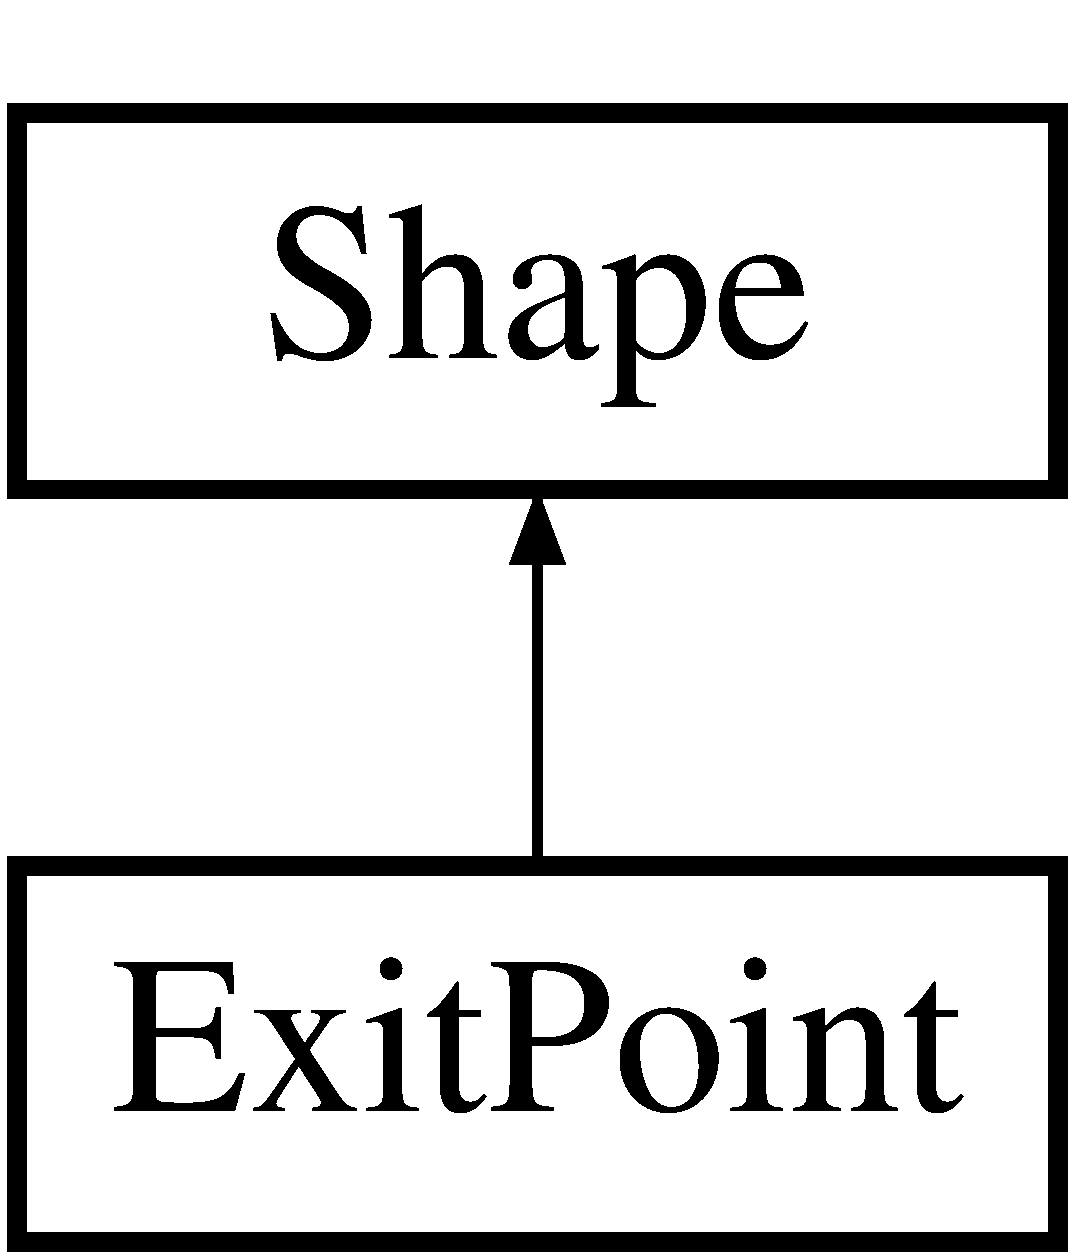
\includegraphics[height=2.000000cm]{class_exit_point}
\end{center}
\end{figure}
\subsection*{Public Member Functions}
\begin{DoxyCompactItemize}
\item 
\mbox{\hyperlink{class_exit_point_ae472f935e952356c9bfe64298474d523}{Exit\+Point}} ()
\item 
\mbox{\hyperlink{class_exit_point_aa764fee5b37cb7dbda6f2fde39ffbc05}{$\sim$\+Exit\+Point}} ()
\item 
void \mbox{\hyperlink{class_exit_point_a2762c0c61bbe71a1a292b86e9517e860}{find\+Exit\+Point}} (const Mat \&img)
\item 
std\+::vector$<$ cv\+::\+Point $>$ \mbox{\hyperlink{class_exit_point_ac26a595a35b370cf7375874395715af0}{get\+Corners}} ()
\item 
void \mbox{\hyperlink{class_exit_point_aff4341c31734d77224b1251988949430}{set\+Corners}} (std\+::vector$<$ cv\+::\+Point $>$ corners)
\item 
cv\+::\+Point \mbox{\hyperlink{class_exit_point_ad373de21603871832e10568631ef3cda}{get\+Top\+Left}} ()
\item 
void \mbox{\hyperlink{class_exit_point_a31c88803968c8b215062b97b699721e2}{set\+Top\+Left}} (cv\+::\+Point top\+Left)
\item 
cv\+::\+Point \mbox{\hyperlink{class_exit_point_a448716aa575ba751f72ab0f437b6a138}{get\+Top\+Right}} ()
\item 
void \mbox{\hyperlink{class_exit_point_ae27c395eb18321cb120b99ffbed6028a}{set\+Top\+Right}} (cv\+::\+Point top\+Right)
\item 
cv\+::\+Point \mbox{\hyperlink{class_exit_point_a51ac01267f39908e468ec859ba8d3096}{get\+Bottom\+Left}} ()
\item 
void \mbox{\hyperlink{class_exit_point_a22bf3a433b3567d36463699e16aaa86b}{set\+Bottom\+Left}} (cv\+::\+Point bottom\+Left)
\item 
cv\+::\+Point \mbox{\hyperlink{class_exit_point_a7a0e9d613aa361083bd4bf91f2080398}{get\+Bottom\+Right}} ()
\item 
void \mbox{\hyperlink{class_exit_point_afe10f2b0cf00b654dc1c95183462ed1a}{set\+Bottom\+Right}} (cv\+::\+Point bottom\+Right)
\end{DoxyCompactItemize}


\subsection{Detailed Description}
\mbox{\hyperlink{class_exit_point}{Exit\+Point}} class is able to detect and save the exit point given a photo 

\subsection{Constructor \& Destructor Documentation}
\mbox{\Hypertarget{class_exit_point_ae472f935e952356c9bfe64298474d523}\label{class_exit_point_ae472f935e952356c9bfe64298474d523}} 
\index{Exit\+Point@{Exit\+Point}!Exit\+Point@{Exit\+Point}}
\index{Exit\+Point@{Exit\+Point}!Exit\+Point@{Exit\+Point}}
\subsubsection{\texorpdfstring{Exit\+Point()}{ExitPoint()}}
{\footnotesize\ttfamily Exit\+Point\+::\+Exit\+Point (\begin{DoxyParamCaption}{ }\end{DoxyParamCaption})}

constructor of the \mbox{\hyperlink{class_exit_point}{Exit\+Point}} class \mbox{\Hypertarget{class_exit_point_aa764fee5b37cb7dbda6f2fde39ffbc05}\label{class_exit_point_aa764fee5b37cb7dbda6f2fde39ffbc05}} 
\index{Exit\+Point@{Exit\+Point}!````~Exit\+Point@{$\sim$\+Exit\+Point}}
\index{````~Exit\+Point@{$\sim$\+Exit\+Point}!Exit\+Point@{Exit\+Point}}
\subsubsection{\texorpdfstring{$\sim$\+Exit\+Point()}{~ExitPoint()}}
{\footnotesize\ttfamily Exit\+Point\+::$\sim$\+Exit\+Point (\begin{DoxyParamCaption}{ }\end{DoxyParamCaption})}

destructor of the \mbox{\hyperlink{class_exit_point}{Exit\+Point}} class 

\subsection{Member Function Documentation}
\mbox{\Hypertarget{class_exit_point_a2762c0c61bbe71a1a292b86e9517e860}\label{class_exit_point_a2762c0c61bbe71a1a292b86e9517e860}} 
\index{Exit\+Point@{Exit\+Point}!find\+Exit\+Point@{find\+Exit\+Point}}
\index{find\+Exit\+Point@{find\+Exit\+Point}!Exit\+Point@{Exit\+Point}}
\subsubsection{\texorpdfstring{find\+Exit\+Point()}{findExitPoint()}}
{\footnotesize\ttfamily void Exit\+Point\+::find\+Exit\+Point (\begin{DoxyParamCaption}\item[{const Mat \&}]{img }\end{DoxyParamCaption})}

retrieve and set the corners in the \mbox{\hyperlink{class_exit_point}{Exit\+Point}} object 
\begin{DoxyParams}{Parameters}
{\em img} & image of the arena \\
\hline
\end{DoxyParams}
\mbox{\Hypertarget{class_exit_point_a51ac01267f39908e468ec859ba8d3096}\label{class_exit_point_a51ac01267f39908e468ec859ba8d3096}} 
\index{Exit\+Point@{Exit\+Point}!get\+Bottom\+Left@{get\+Bottom\+Left}}
\index{get\+Bottom\+Left@{get\+Bottom\+Left}!Exit\+Point@{Exit\+Point}}
\subsubsection{\texorpdfstring{get\+Bottom\+Left()}{getBottomLeft()}}
{\footnotesize\ttfamily cv\+::\+Point Exit\+Point\+::get\+Bottom\+Left (\begin{DoxyParamCaption}{ }\end{DoxyParamCaption})}

return the bottom left corner \begin{DoxyReturn}{Returns}
the bottom left corner 
\end{DoxyReturn}
\mbox{\Hypertarget{class_exit_point_a7a0e9d613aa361083bd4bf91f2080398}\label{class_exit_point_a7a0e9d613aa361083bd4bf91f2080398}} 
\index{Exit\+Point@{Exit\+Point}!get\+Bottom\+Right@{get\+Bottom\+Right}}
\index{get\+Bottom\+Right@{get\+Bottom\+Right}!Exit\+Point@{Exit\+Point}}
\subsubsection{\texorpdfstring{get\+Bottom\+Right()}{getBottomRight()}}
{\footnotesize\ttfamily cv\+::\+Point Exit\+Point\+::get\+Bottom\+Right (\begin{DoxyParamCaption}{ }\end{DoxyParamCaption})}

return the bottom right corner of the exit point \begin{DoxyReturn}{Returns}
bottom right corner of the exit point 
\end{DoxyReturn}
\mbox{\Hypertarget{class_exit_point_ac26a595a35b370cf7375874395715af0}\label{class_exit_point_ac26a595a35b370cf7375874395715af0}} 
\index{Exit\+Point@{Exit\+Point}!get\+Corners@{get\+Corners}}
\index{get\+Corners@{get\+Corners}!Exit\+Point@{Exit\+Point}}
\subsubsection{\texorpdfstring{get\+Corners()}{getCorners()}}
{\footnotesize\ttfamily std\+::vector$<$cv\+::\+Point$>$ Exit\+Point\+::get\+Corners (\begin{DoxyParamCaption}{ }\end{DoxyParamCaption})}

return a list of corners in a clockwise order \begin{DoxyReturn}{Returns}
list of corners in a clockwise order 
\end{DoxyReturn}
\mbox{\Hypertarget{class_exit_point_ad373de21603871832e10568631ef3cda}\label{class_exit_point_ad373de21603871832e10568631ef3cda}} 
\index{Exit\+Point@{Exit\+Point}!get\+Top\+Left@{get\+Top\+Left}}
\index{get\+Top\+Left@{get\+Top\+Left}!Exit\+Point@{Exit\+Point}}
\subsubsection{\texorpdfstring{get\+Top\+Left()}{getTopLeft()}}
{\footnotesize\ttfamily cv\+::\+Point Exit\+Point\+::get\+Top\+Left (\begin{DoxyParamCaption}{ }\end{DoxyParamCaption})}

return the top left corner of the exit point \begin{DoxyReturn}{Returns}
return the top left corner of the exit point 
\end{DoxyReturn}
\mbox{\Hypertarget{class_exit_point_a448716aa575ba751f72ab0f437b6a138}\label{class_exit_point_a448716aa575ba751f72ab0f437b6a138}} 
\index{Exit\+Point@{Exit\+Point}!get\+Top\+Right@{get\+Top\+Right}}
\index{get\+Top\+Right@{get\+Top\+Right}!Exit\+Point@{Exit\+Point}}
\subsubsection{\texorpdfstring{get\+Top\+Right()}{getTopRight()}}
{\footnotesize\ttfamily cv\+::\+Point Exit\+Point\+::get\+Top\+Right (\begin{DoxyParamCaption}{ }\end{DoxyParamCaption})}

return the top right corner of the exit point \begin{DoxyReturn}{Returns}
return the top right corner of the exit point 
\end{DoxyReturn}
\mbox{\Hypertarget{class_exit_point_a22bf3a433b3567d36463699e16aaa86b}\label{class_exit_point_a22bf3a433b3567d36463699e16aaa86b}} 
\index{Exit\+Point@{Exit\+Point}!set\+Bottom\+Left@{set\+Bottom\+Left}}
\index{set\+Bottom\+Left@{set\+Bottom\+Left}!Exit\+Point@{Exit\+Point}}
\subsubsection{\texorpdfstring{set\+Bottom\+Left()}{setBottomLeft()}}
{\footnotesize\ttfamily void Exit\+Point\+::set\+Bottom\+Left (\begin{DoxyParamCaption}\item[{cv\+::\+Point}]{bottom\+Left }\end{DoxyParamCaption})}

set the bottom left corner 
\begin{DoxyParams}{Parameters}
{\em bottom\+Left} & bottom left corner of the exit point \\
\hline
\end{DoxyParams}
\mbox{\Hypertarget{class_exit_point_afe10f2b0cf00b654dc1c95183462ed1a}\label{class_exit_point_afe10f2b0cf00b654dc1c95183462ed1a}} 
\index{Exit\+Point@{Exit\+Point}!set\+Bottom\+Right@{set\+Bottom\+Right}}
\index{set\+Bottom\+Right@{set\+Bottom\+Right}!Exit\+Point@{Exit\+Point}}
\subsubsection{\texorpdfstring{set\+Bottom\+Right()}{setBottomRight()}}
{\footnotesize\ttfamily void Exit\+Point\+::set\+Bottom\+Right (\begin{DoxyParamCaption}\item[{cv\+::\+Point}]{bottom\+Right }\end{DoxyParamCaption})}

set the bottom right corner 
\begin{DoxyParams}{Parameters}
{\em bottom\+Right} & bottom right corner of the exit point \\
\hline
\end{DoxyParams}
\mbox{\Hypertarget{class_exit_point_aff4341c31734d77224b1251988949430}\label{class_exit_point_aff4341c31734d77224b1251988949430}} 
\index{Exit\+Point@{Exit\+Point}!set\+Corners@{set\+Corners}}
\index{set\+Corners@{set\+Corners}!Exit\+Point@{Exit\+Point}}
\subsubsection{\texorpdfstring{set\+Corners()}{setCorners()}}
{\footnotesize\ttfamily void Exit\+Point\+::set\+Corners (\begin{DoxyParamCaption}\item[{std\+::vector$<$ cv\+::\+Point $>$}]{corners }\end{DoxyParamCaption})}

set the list of corners 
\begin{DoxyParams}{Parameters}
{\em corners} & list of corners that have to be setted \\
\hline
\end{DoxyParams}
\mbox{\Hypertarget{class_exit_point_a31c88803968c8b215062b97b699721e2}\label{class_exit_point_a31c88803968c8b215062b97b699721e2}} 
\index{Exit\+Point@{Exit\+Point}!set\+Top\+Left@{set\+Top\+Left}}
\index{set\+Top\+Left@{set\+Top\+Left}!Exit\+Point@{Exit\+Point}}
\subsubsection{\texorpdfstring{set\+Top\+Left()}{setTopLeft()}}
{\footnotesize\ttfamily void Exit\+Point\+::set\+Top\+Left (\begin{DoxyParamCaption}\item[{cv\+::\+Point}]{top\+Left }\end{DoxyParamCaption})}

set the top left corner 
\begin{DoxyParams}{Parameters}
{\em top\+Left} & top left corner that has to be setted \\
\hline
\end{DoxyParams}
\mbox{\Hypertarget{class_exit_point_ae27c395eb18321cb120b99ffbed6028a}\label{class_exit_point_ae27c395eb18321cb120b99ffbed6028a}} 
\index{Exit\+Point@{Exit\+Point}!set\+Top\+Right@{set\+Top\+Right}}
\index{set\+Top\+Right@{set\+Top\+Right}!Exit\+Point@{Exit\+Point}}
\subsubsection{\texorpdfstring{set\+Top\+Right()}{setTopRight()}}
{\footnotesize\ttfamily void Exit\+Point\+::set\+Top\+Right (\begin{DoxyParamCaption}\item[{cv\+::\+Point}]{top\+Right }\end{DoxyParamCaption})}

set the top right corner 
\begin{DoxyParams}{Parameters}
{\em top\+Right} & top right corner tha has to be setted \\
\hline
\end{DoxyParams}


The documentation for this class was generated from the following file\+:\begin{DoxyCompactItemize}
\item 
Exit\+Point.\+hpp\end{DoxyCompactItemize}

\hypertarget{class_hexagon}{}\section{Hexagon Class Reference}
\label{class_hexagon}\index{Hexagon@{Hexagon}}


Class for handling hexagon obstacles.  




{\ttfamily \#include $<$Hexagon.\+hpp$>$}

Inheritance diagram for Hexagon\+:\begin{figure}[H]
\begin{center}
\leavevmode
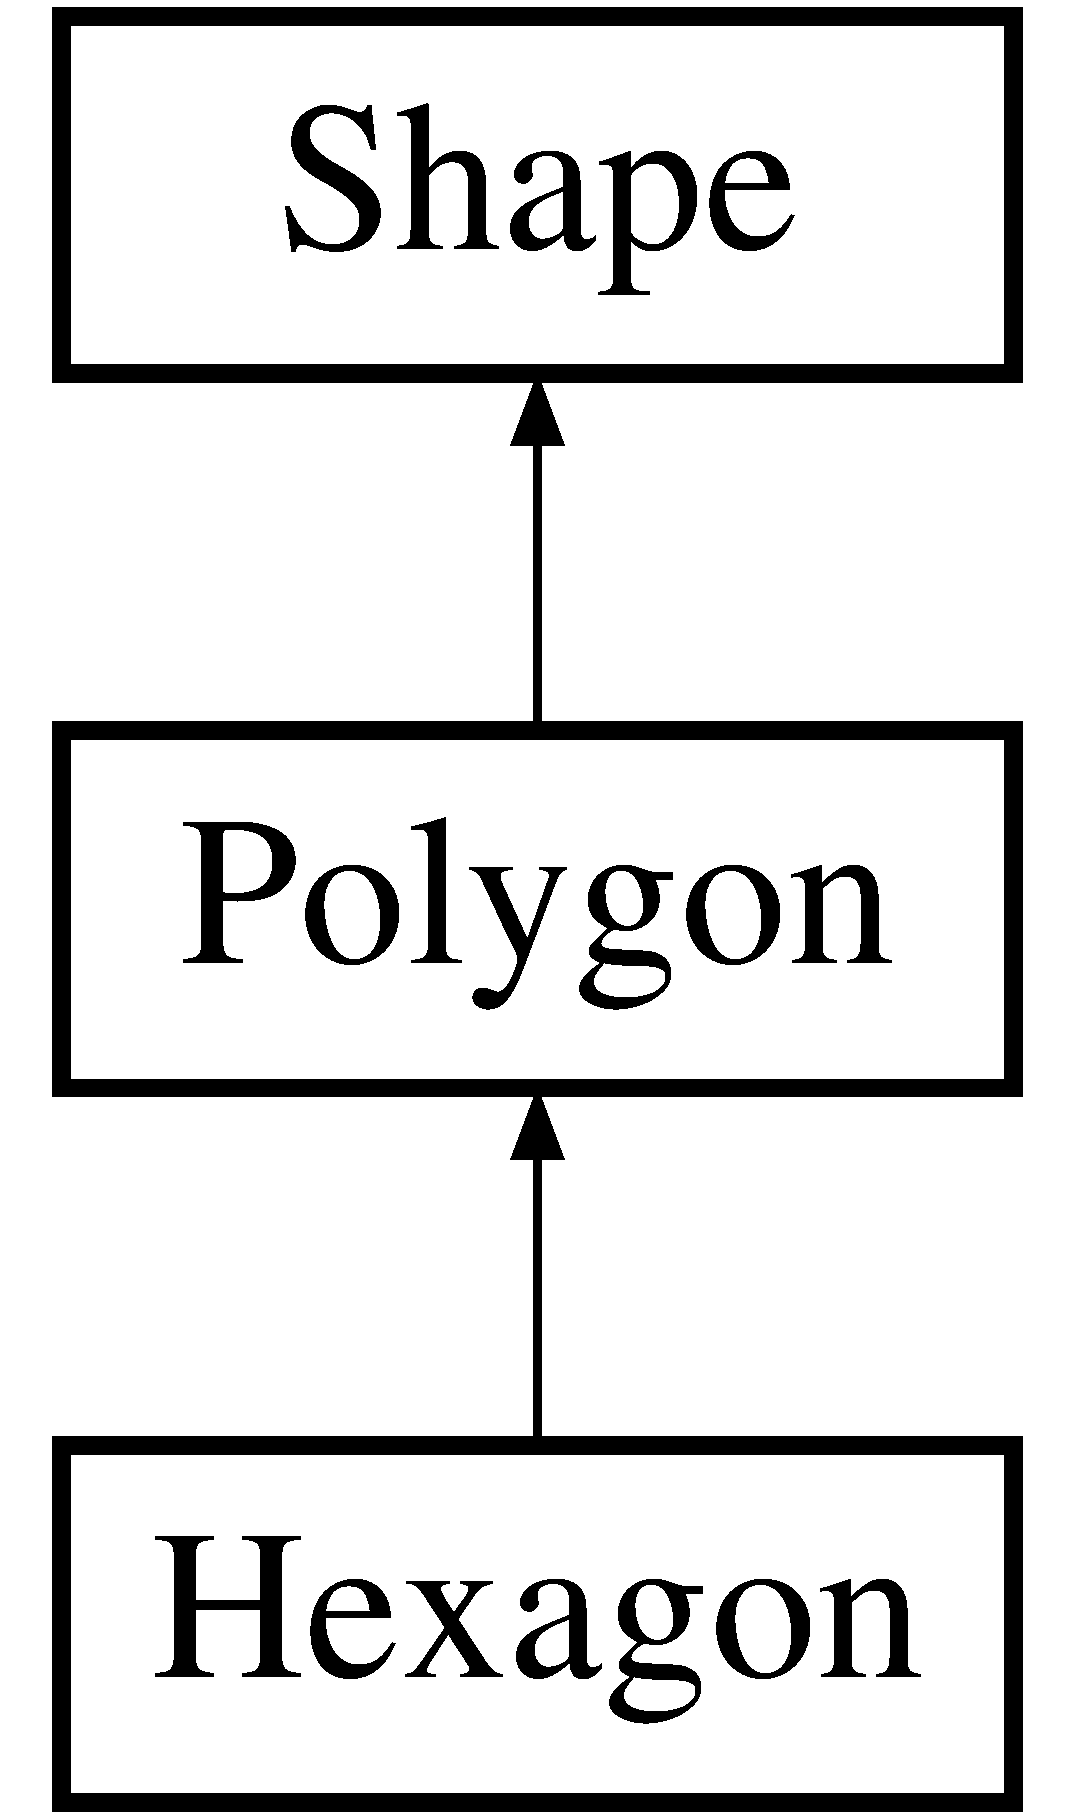
\includegraphics[height=3.000000cm]{class_hexagon}
\end{center}
\end{figure}
\subsection*{Public Member Functions}
\begin{DoxyCompactItemize}
\item 
\mbox{\hyperlink{class_hexagon_ab503950412a7f11dab9c697c45b614a2}{Hexagon}} ()
\item 
\mbox{\Hypertarget{class_hexagon_aaed01ef0ea21f3533fcd73a660326ab3}\label{class_hexagon_aaed01ef0ea21f3533fcd73a660326ab3}} 
{\bfseries Hexagon} (std\+::vector$<$ cv\+::\+Point $>$ \mbox{\hyperlink{class_polygon_a347474823f6113a34fdefeee276d1b9e}{points}})
\item 
\mbox{\hyperlink{class_hexagon_aaaa69a37657fe47cad3c17d7c3569318}{$\sim$\+Hexagon}} ()
\item 
std\+::vector$<$ cv\+::\+Point $>$ \mbox{\hyperlink{class_hexagon_aa12df068505254931530cbe74ac85ad0}{get\+Corners}} ()
\item 
void \mbox{\hyperlink{class_hexagon_a1b5cdb94637901f346373429660af3b1}{set\+Corners}} (std\+::vector$<$ cv\+::\+Point $>$ corners)
\item 
\mbox{\Hypertarget{class_hexagon_a59383ce16764b0123ccde0e8db32cf06}\label{class_hexagon_a59383ce16764b0123ccde0e8db32cf06}} 
void \mbox{\hyperlink{class_hexagon_a59383ce16764b0123ccde0e8db32cf06}{assign\+\_\+points}} ()
\begin{DoxyCompactList}\small\item\em assignes the points \end{DoxyCompactList}\end{DoxyCompactItemize}
\subsection*{Additional Inherited Members}


\subsection{Detailed Description}
Class for handling hexagon obstacles. 

\subsection{Constructor \& Destructor Documentation}
\mbox{\Hypertarget{class_hexagon_ab503950412a7f11dab9c697c45b614a2}\label{class_hexagon_ab503950412a7f11dab9c697c45b614a2}} 
\index{Hexagon@{Hexagon}!Hexagon@{Hexagon}}
\index{Hexagon@{Hexagon}!Hexagon@{Hexagon}}
\subsubsection{\texorpdfstring{Hexagon()}{Hexagon()}}
{\footnotesize\ttfamily Hexagon\+::\+Hexagon (\begin{DoxyParamCaption}{ }\end{DoxyParamCaption})}

constructor of the \mbox{\hyperlink{class_hexagon}{Hexagon}} class \mbox{\Hypertarget{class_hexagon_aaaa69a37657fe47cad3c17d7c3569318}\label{class_hexagon_aaaa69a37657fe47cad3c17d7c3569318}} 
\index{Hexagon@{Hexagon}!````~Hexagon@{$\sim$\+Hexagon}}
\index{````~Hexagon@{$\sim$\+Hexagon}!Hexagon@{Hexagon}}
\subsubsection{\texorpdfstring{$\sim$\+Hexagon()}{~Hexagon()}}
{\footnotesize\ttfamily Hexagon\+::$\sim$\+Hexagon (\begin{DoxyParamCaption}{ }\end{DoxyParamCaption})}

destructor of the \mbox{\hyperlink{class_hexagon}{Hexagon}} class 

\subsection{Member Function Documentation}
\mbox{\Hypertarget{class_hexagon_aa12df068505254931530cbe74ac85ad0}\label{class_hexagon_aa12df068505254931530cbe74ac85ad0}} 
\index{Hexagon@{Hexagon}!get\+Corners@{get\+Corners}}
\index{get\+Corners@{get\+Corners}!Hexagon@{Hexagon}}
\subsubsection{\texorpdfstring{get\+Corners()}{getCorners()}}
{\footnotesize\ttfamily std\+::vector$<$cv\+::\+Point$>$ Hexagon\+::get\+Corners (\begin{DoxyParamCaption}{ }\end{DoxyParamCaption})}

return a list of corners of the hexagon \begin{DoxyReturn}{Returns}
list of corners of the hexagon 
\end{DoxyReturn}
\mbox{\Hypertarget{class_hexagon_a1b5cdb94637901f346373429660af3b1}\label{class_hexagon_a1b5cdb94637901f346373429660af3b1}} 
\index{Hexagon@{Hexagon}!set\+Corners@{set\+Corners}}
\index{set\+Corners@{set\+Corners}!Hexagon@{Hexagon}}
\subsubsection{\texorpdfstring{set\+Corners()}{setCorners()}}
{\footnotesize\ttfamily void Hexagon\+::set\+Corners (\begin{DoxyParamCaption}\item[{std\+::vector$<$ cv\+::\+Point $>$}]{corners }\end{DoxyParamCaption})}

set the list of corners 
\begin{DoxyParams}{Parameters}
{\em corners} & list of corners \\
\hline
\end{DoxyParams}


The documentation for this class was generated from the following file\+:\begin{DoxyCompactItemize}
\item 
Hexagon.\+hpp\end{DoxyCompactItemize}

\hypertarget{struct_h_s_v_filter_range}{}\section{H\+S\+V\+Filter\+Range Struct Reference}
\label{struct_h_s_v_filter_range}\index{H\+S\+V\+Filter\+Range@{H\+S\+V\+Filter\+Range}}
\subsection*{Public Member Functions}
\begin{DoxyCompactItemize}
\item 
\mbox{\Hypertarget{struct_h_s_v_filter_range_a4e37551e92211618e217752f0056847a}\label{struct_h_s_v_filter_range_a4e37551e92211618e217752f0056847a}} 
{\bfseries H\+S\+V\+Filter\+Range} (std\+::string quality)
\end{DoxyCompactItemize}
\subsection*{Public Attributes}
\begin{DoxyCompactItemize}
\item 
\mbox{\Hypertarget{struct_h_s_v_filter_range_a1c5b705f9992e014fd4dd7085e078c9d}\label{struct_h_s_v_filter_range_a1c5b705f9992e014fd4dd7085e078c9d}} 
cv\+::\+Scalar {\bfseries ub} = cv\+::\+Scalar(90, 255, 255)
\item 
\mbox{\Hypertarget{struct_h_s_v_filter_range_a0c5c2a10fb591c4dd1512ae81e1032a4}\label{struct_h_s_v_filter_range_a0c5c2a10fb591c4dd1512ae81e1032a4}} 
cv\+::\+Scalar {\bfseries lb} = cv\+::\+Scalar(48, 53, 102)
\item 
\mbox{\Hypertarget{struct_h_s_v_filter_range_a5ded3fde3f4b37d5e0de6f40fd508271}\label{struct_h_s_v_filter_range_a5ded3fde3f4b37d5e0de6f40fd508271}} 
std\+::string {\bfseries saved\+\_\+quality} = \char`\"{}bad\char`\"{}
\end{DoxyCompactItemize}


The documentation for this struct was generated from the following file\+:\begin{DoxyCompactItemize}
\item 
Color\+\_\+\+Processing.\+hpp\end{DoxyCompactItemize}

\hypertarget{class_inverse___perspective___mapping}{}\section{Inverse\+\_\+\+Perspective\+\_\+\+Mapping Class Reference}
\label{class_inverse___perspective___mapping}\index{Inverse\+\_\+\+Perspective\+\_\+\+Mapping@{Inverse\+\_\+\+Perspective\+\_\+\+Mapping}}


{\ttfamily \#include $<$Inverse\+\_\+\+Perspective\+\_\+\+Mapping.\+hpp$>$}

\subsection*{Public Member Functions}
\begin{DoxyCompactItemize}
\item 
\mbox{\hyperlink{class_inverse___perspective___mapping_a9c3733e22a6516e932a2197196c999f2}{Inverse\+\_\+\+Perspective\+\_\+\+Mapping}} ()
\item 
\mbox{\hyperlink{class_inverse___perspective___mapping_a9f1588ec3a84a4c664ae33c1fd3693df}{$\sim$\+Inverse\+\_\+\+Perspective\+\_\+\+Mapping}} ()
\item 
void \mbox{\hyperlink{class_inverse___perspective___mapping_a60f8dbac68fadb20b085bfbcef293480}{load\+Coefficients}} (const std\+::string \&filename, cv\+::\+Mat \&camera\+\_\+matrix, cv\+::\+Mat \&dist\+\_\+coeffs)
\item 
Mat \mbox{\hyperlink{class_inverse___perspective___mapping_aa4444fc0f5e10cab7f408d6679be73db}{find\+Transform}} (const std\+::string \&calib\+\_\+image\+\_\+name, const cv\+::\+Mat \&camera\+\_\+matrix, const cv\+::\+Mat \&dist\+\_\+coeffs, double \&pixel\+\_\+scale, cv\+::\+Mat \&persp\+\_\+img)
\item 
void \mbox{\hyperlink{class_inverse___perspective___mapping_abdea95329f3868f2a0875832a67f1076}{store\+All\+Parameters}} (const std\+::string \&filename, const cv\+::\+Mat \&camera\+\_\+matrix, const cv\+::\+Mat \&dist\+\_\+coeffs, double pixel\+\_\+scale, const Mat \&persp\+\_\+transf)
\item 
cv\+::\+Mat \mbox{\hyperlink{class_inverse___perspective___mapping_ad95385fefc56350a732760d7c68fe6a3}{run}} (std\+::string intrinsic\+\_\+conf, std\+::string image, std\+::string outputfilename)
\end{DoxyCompactItemize}


\subsection{Detailed Description}
produce a perspective transformation around the arena given a photo 

\subsection{Constructor \& Destructor Documentation}
\mbox{\Hypertarget{class_inverse___perspective___mapping_a9c3733e22a6516e932a2197196c999f2}\label{class_inverse___perspective___mapping_a9c3733e22a6516e932a2197196c999f2}} 
\index{Inverse\+\_\+\+Perspective\+\_\+\+Mapping@{Inverse\+\_\+\+Perspective\+\_\+\+Mapping}!Inverse\+\_\+\+Perspective\+\_\+\+Mapping@{Inverse\+\_\+\+Perspective\+\_\+\+Mapping}}
\index{Inverse\+\_\+\+Perspective\+\_\+\+Mapping@{Inverse\+\_\+\+Perspective\+\_\+\+Mapping}!Inverse\+\_\+\+Perspective\+\_\+\+Mapping@{Inverse\+\_\+\+Perspective\+\_\+\+Mapping}}
\subsubsection{\texorpdfstring{Inverse\+\_\+\+Perspective\+\_\+\+Mapping()}{Inverse\_Perspective\_Mapping()}}
{\footnotesize\ttfamily Inverse\+\_\+\+Perspective\+\_\+\+Mapping\+::\+Inverse\+\_\+\+Perspective\+\_\+\+Mapping (\begin{DoxyParamCaption}{ }\end{DoxyParamCaption})}

constructor of inverse perspective mapping class \mbox{\Hypertarget{class_inverse___perspective___mapping_a9f1588ec3a84a4c664ae33c1fd3693df}\label{class_inverse___perspective___mapping_a9f1588ec3a84a4c664ae33c1fd3693df}} 
\index{Inverse\+\_\+\+Perspective\+\_\+\+Mapping@{Inverse\+\_\+\+Perspective\+\_\+\+Mapping}!````~Inverse\+\_\+\+Perspective\+\_\+\+Mapping@{$\sim$\+Inverse\+\_\+\+Perspective\+\_\+\+Mapping}}
\index{````~Inverse\+\_\+\+Perspective\+\_\+\+Mapping@{$\sim$\+Inverse\+\_\+\+Perspective\+\_\+\+Mapping}!Inverse\+\_\+\+Perspective\+\_\+\+Mapping@{Inverse\+\_\+\+Perspective\+\_\+\+Mapping}}
\subsubsection{\texorpdfstring{$\sim$\+Inverse\+\_\+\+Perspective\+\_\+\+Mapping()}{~Inverse\_Perspective\_Mapping()}}
{\footnotesize\ttfamily Inverse\+\_\+\+Perspective\+\_\+\+Mapping\+::$\sim$\+Inverse\+\_\+\+Perspective\+\_\+\+Mapping (\begin{DoxyParamCaption}{ }\end{DoxyParamCaption})}

destructor of inverse perspective mapping class 

\subsection{Member Function Documentation}
\mbox{\Hypertarget{class_inverse___perspective___mapping_aa4444fc0f5e10cab7f408d6679be73db}\label{class_inverse___perspective___mapping_aa4444fc0f5e10cab7f408d6679be73db}} 
\index{Inverse\+\_\+\+Perspective\+\_\+\+Mapping@{Inverse\+\_\+\+Perspective\+\_\+\+Mapping}!find\+Transform@{find\+Transform}}
\index{find\+Transform@{find\+Transform}!Inverse\+\_\+\+Perspective\+\_\+\+Mapping@{Inverse\+\_\+\+Perspective\+\_\+\+Mapping}}
\subsubsection{\texorpdfstring{find\+Transform()}{findTransform()}}
{\footnotesize\ttfamily Mat Inverse\+\_\+\+Perspective\+\_\+\+Mapping\+::find\+Transform (\begin{DoxyParamCaption}\item[{const std\+::string \&}]{calib\+\_\+image\+\_\+name,  }\item[{const cv\+::\+Mat \&}]{camera\+\_\+matrix,  }\item[{const cv\+::\+Mat \&}]{dist\+\_\+coeffs,  }\item[{double \&}]{pixel\+\_\+scale,  }\item[{cv\+::\+Mat \&}]{persp\+\_\+img }\end{DoxyParamCaption})}

function to determine the perspective transformation of a rectangle on the ground plane 
\begin{DoxyParams}{Parameters}
{\em calib\+\_\+image\+\_\+name} & image \\
\hline
{\em camera\+\_\+matrix} & camera matrix \\
\hline
{\em dist\+\_\+coeffs} & distortion coefficents \\
\hline
{\em pixel\+\_\+scale} & pixel scaling \\
\hline
{\em persp\+\_\+img} & image after trasformation \\
\hline
\end{DoxyParams}
\begin{DoxyReturn}{Returns}

\end{DoxyReturn}
\mbox{\Hypertarget{class_inverse___perspective___mapping_a60f8dbac68fadb20b085bfbcef293480}\label{class_inverse___perspective___mapping_a60f8dbac68fadb20b085bfbcef293480}} 
\index{Inverse\+\_\+\+Perspective\+\_\+\+Mapping@{Inverse\+\_\+\+Perspective\+\_\+\+Mapping}!load\+Coefficients@{load\+Coefficients}}
\index{load\+Coefficients@{load\+Coefficients}!Inverse\+\_\+\+Perspective\+\_\+\+Mapping@{Inverse\+\_\+\+Perspective\+\_\+\+Mapping}}
\subsubsection{\texorpdfstring{load\+Coefficients()}{loadCoefficients()}}
{\footnotesize\ttfamily void Inverse\+\_\+\+Perspective\+\_\+\+Mapping\+::load\+Coefficients (\begin{DoxyParamCaption}\item[{const std\+::string \&}]{filename,  }\item[{cv\+::\+Mat \&}]{camera\+\_\+matrix,  }\item[{cv\+::\+Mat \&}]{dist\+\_\+coeffs }\end{DoxyParamCaption})}


\begin{DoxyParams}{Parameters}
{\em filename} & intrinsic calibration file name \\
\hline
{\em camera\+\_\+matrix} & camerat matrix file \\
\hline
{\em dist\+\_\+coeffs} & distortion coefficients \\
\hline
\end{DoxyParams}
\mbox{\Hypertarget{class_inverse___perspective___mapping_ad95385fefc56350a732760d7c68fe6a3}\label{class_inverse___perspective___mapping_ad95385fefc56350a732760d7c68fe6a3}} 
\index{Inverse\+\_\+\+Perspective\+\_\+\+Mapping@{Inverse\+\_\+\+Perspective\+\_\+\+Mapping}!run@{run}}
\index{run@{run}!Inverse\+\_\+\+Perspective\+\_\+\+Mapping@{Inverse\+\_\+\+Perspective\+\_\+\+Mapping}}
\subsubsection{\texorpdfstring{run()}{run()}}
{\footnotesize\ttfamily cv\+::\+Mat Inverse\+\_\+\+Perspective\+\_\+\+Mapping\+::run (\begin{DoxyParamCaption}\item[{std\+::string}]{intrinsic\+\_\+conf,  }\item[{std\+::string}]{image,  }\item[{std\+::string}]{outputfilename }\end{DoxyParamCaption})}

perform a perspective transformation 
\begin{DoxyParams}{Parameters}
{\em intrinsic\+\_\+conf} & \\
\hline
{\em image} & \\
\hline
{\em outputfilename} & \\
\hline
\end{DoxyParams}
\begin{DoxyReturn}{Returns}
the image after transformation 
\end{DoxyReturn}
\mbox{\Hypertarget{class_inverse___perspective___mapping_abdea95329f3868f2a0875832a67f1076}\label{class_inverse___perspective___mapping_abdea95329f3868f2a0875832a67f1076}} 
\index{Inverse\+\_\+\+Perspective\+\_\+\+Mapping@{Inverse\+\_\+\+Perspective\+\_\+\+Mapping}!store\+All\+Parameters@{store\+All\+Parameters}}
\index{store\+All\+Parameters@{store\+All\+Parameters}!Inverse\+\_\+\+Perspective\+\_\+\+Mapping@{Inverse\+\_\+\+Perspective\+\_\+\+Mapping}}
\subsubsection{\texorpdfstring{store\+All\+Parameters()}{storeAllParameters()}}
{\footnotesize\ttfamily void Inverse\+\_\+\+Perspective\+\_\+\+Mapping\+::store\+All\+Parameters (\begin{DoxyParamCaption}\item[{const std\+::string \&}]{filename,  }\item[{const cv\+::\+Mat \&}]{camera\+\_\+matrix,  }\item[{const cv\+::\+Mat \&}]{dist\+\_\+coeffs,  }\item[{double}]{pixel\+\_\+scale,  }\item[{const Mat \&}]{persp\+\_\+transf }\end{DoxyParamCaption})}

Store all the parameters to a file, for a later use, using the File\+Storage class methods 
\begin{DoxyParams}{Parameters}
{\em filename} & \\
\hline
{\em camera\+\_\+matrix} & \\
\hline
{\em dist\+\_\+coeffs} & \\
\hline
{\em pixel\+\_\+scale} & \\
\hline
{\em persp\+\_\+transf} & \\
\hline
\end{DoxyParams}


The documentation for this class was generated from the following file\+:\begin{DoxyCompactItemize}
\item 
Inverse\+\_\+\+Perspective\+\_\+\+Mapping.\+hpp\end{DoxyCompactItemize}

\hypertarget{class_line}{}\section{Line Class Reference}
\label{class_line}\index{Line@{Line}}


\mbox{\hyperlink{class_line}{Line}} class that describes the basic line of a path.  




{\ttfamily \#include $<$Line.\+hpp$>$}

Inheritance diagram for Line\+:\begin{figure}[H]
\begin{center}
\leavevmode
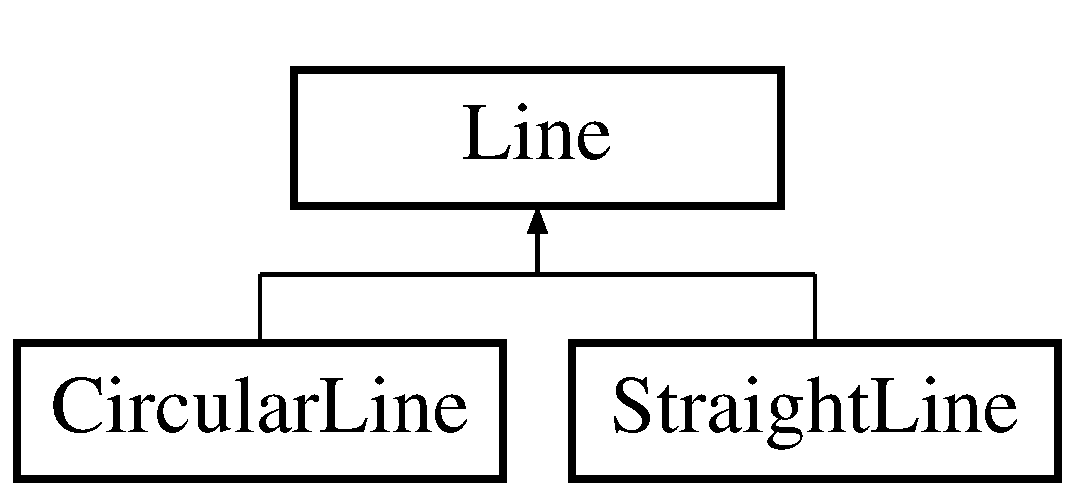
\includegraphics[height=2.000000cm]{class_line}
\end{center}
\end{figure}
\subsection*{Public Member Functions}
\begin{DoxyCompactItemize}
\item 
\mbox{\Hypertarget{class_line_acc11b8a429d8cdd63ba6803dff5602b3}\label{class_line_acc11b8a429d8cdd63ba6803dff5602b3}} 
\mbox{\hyperlink{class_line_acc11b8a429d8cdd63ba6803dff5602b3}{Line}} ()
\begin{DoxyCompactList}\small\item\em constructor of \mbox{\hyperlink{class_line}{Line}} class \end{DoxyCompactList}\item 
\mbox{\hyperlink{class_line_a123e1da8ef560bac5ab6b643e25c3d8f}{Line}} (\mbox{\hyperlink{class_position}{Position}} start\+\_\+point, \mbox{\hyperlink{class_position}{Position}} end\+\_\+point)
\begin{DoxyCompactList}\small\item\em contrusctor of \mbox{\hyperlink{class_line}{Line}} class \end{DoxyCompactList}\item 
\mbox{\Hypertarget{class_line_aabe85f48d22d92b62257091f48174fac}\label{class_line_aabe85f48d22d92b62257091f48174fac}} 
\mbox{\hyperlink{class_line_aabe85f48d22d92b62257091f48174fac}{$\sim$\+Line}} ()
\begin{DoxyCompactList}\small\item\em destructor of the line path \end{DoxyCompactList}\item 
void \mbox{\hyperlink{class_line_a6356eecffc24d5016c9aa697611c3020}{set\+Start\+Point}} (\mbox{\hyperlink{class_position}{Position}} start\+\_\+point\+\_\+i)
\begin{DoxyCompactList}\small\item\em set the start position of the path \end{DoxyCompactList}\item 
\mbox{\hyperlink{class_position}{Position}} \mbox{\hyperlink{class_line_aa9924a540d8ba2da841a414c58dafb56}{get\+Start\+Point}} ()
\begin{DoxyCompactList}\small\item\em return the start point of the path \end{DoxyCompactList}\item 
void \mbox{\hyperlink{class_line_a47359d43675ff78f2b0af8378d952387}{set\+End\+Point}} (\mbox{\hyperlink{class_position}{Position}} end\+\_\+point\+\_\+i)
\begin{DoxyCompactList}\small\item\em set the end point of the path \end{DoxyCompactList}\item 
\mbox{\hyperlink{class_position}{Position}} \mbox{\hyperlink{class_line_a5f22705f0019c1f855f095ea6b7c4b45}{get\+End\+Point}} ()
\begin{DoxyCompactList}\small\item\em return the end point of the path \end{DoxyCompactList}\item 
void \mbox{\hyperlink{class_line_a387afc9536a3c054dec9eb54f45ea993}{set\+Length}} (double length\+\_\+i)
\begin{DoxyCompactList}\small\item\em set the length of the path \end{DoxyCompactList}\item 
double \mbox{\hyperlink{class_line_a9f91895c2a71dcb2c8da5dd5b057b14a}{get\+Length}} ()
\item 
\mbox{\hyperlink{class_position}{Position}} \mbox{\hyperlink{class_line_ad19714c8b94997c96d35fefaa2bbda26}{find\+End\+Point}} (double k, \mbox{\hyperlink{class_position}{Position}} start, double length)
\begin{DoxyCompactList}\small\item\em function that given the curvature the start point and the lenght of the path allow to find the end point of the line \end{DoxyCompactList}\item 
double \mbox{\hyperlink{class_line_a4976ad80d3fe4a789bac7a1916543edd}{sinc}} (double inp)
\begin{DoxyCompactList}\small\item\em Implementation of function sinc(t), returning 1 for t==0, and sin(t)/t. \end{DoxyCompactList}\item 
double \mbox{\hyperlink{class_line_aa30f3bd50c4de544874c4aaad0a24c6a}{mod2pi}} (double ang)
\begin{DoxyCompactList}\small\item\em Normalize an angle (in range \mbox{[}0,2$\ast$pi)) \end{DoxyCompactList}\end{DoxyCompactItemize}


\subsection{Detailed Description}
\mbox{\hyperlink{class_line}{Line}} class that describes the basic line of a path. 

\subsection{Constructor \& Destructor Documentation}
\mbox{\Hypertarget{class_line_a123e1da8ef560bac5ab6b643e25c3d8f}\label{class_line_a123e1da8ef560bac5ab6b643e25c3d8f}} 
\index{Line@{Line}!Line@{Line}}
\index{Line@{Line}!Line@{Line}}
\subsubsection{\texorpdfstring{Line()}{Line()}}
{\footnotesize\ttfamily Line\+::\+Line (\begin{DoxyParamCaption}\item[{\mbox{\hyperlink{class_position}{Position}}}]{start\+\_\+point,  }\item[{\mbox{\hyperlink{class_position}{Position}}}]{end\+\_\+point }\end{DoxyParamCaption})}



contrusctor of \mbox{\hyperlink{class_line}{Line}} class 


\begin{DoxyParams}{Parameters}
{\em start\+\_\+point} & start point of the path \\
\hline
{\em end\+\_\+point} & end point of the path \\
\hline
\end{DoxyParams}


\subsection{Member Function Documentation}
\mbox{\Hypertarget{class_line_ad19714c8b94997c96d35fefaa2bbda26}\label{class_line_ad19714c8b94997c96d35fefaa2bbda26}} 
\index{Line@{Line}!find\+End\+Point@{find\+End\+Point}}
\index{find\+End\+Point@{find\+End\+Point}!Line@{Line}}
\subsubsection{\texorpdfstring{find\+End\+Point()}{findEndPoint()}}
{\footnotesize\ttfamily \mbox{\hyperlink{class_position}{Position}} Line\+::find\+End\+Point (\begin{DoxyParamCaption}\item[{double}]{k,  }\item[{\mbox{\hyperlink{class_position}{Position}}}]{start,  }\item[{double}]{length }\end{DoxyParamCaption})}



function that given the curvature the start point and the lenght of the path allow to find the end point of the line 


\begin{DoxyParams}{Parameters}
{\em k} & curvature \\
\hline
{\em start} & start point of the line \\
\hline
{\em length} & length of the line \\
\hline
\end{DoxyParams}
\begin{DoxyReturn}{Returns}

\end{DoxyReturn}
\mbox{\Hypertarget{class_line_a5f22705f0019c1f855f095ea6b7c4b45}\label{class_line_a5f22705f0019c1f855f095ea6b7c4b45}} 
\index{Line@{Line}!get\+End\+Point@{get\+End\+Point}}
\index{get\+End\+Point@{get\+End\+Point}!Line@{Line}}
\subsubsection{\texorpdfstring{get\+End\+Point()}{getEndPoint()}}
{\footnotesize\ttfamily \mbox{\hyperlink{class_position}{Position}} Line\+::get\+End\+Point (\begin{DoxyParamCaption}{ }\end{DoxyParamCaption})}



return the end point of the path 

\begin{DoxyReturn}{Returns}
the end point of the path 
\end{DoxyReturn}
\mbox{\Hypertarget{class_line_a9f91895c2a71dcb2c8da5dd5b057b14a}\label{class_line_a9f91895c2a71dcb2c8da5dd5b057b14a}} 
\index{Line@{Line}!get\+Length@{get\+Length}}
\index{get\+Length@{get\+Length}!Line@{Line}}
\subsubsection{\texorpdfstring{get\+Length()}{getLength()}}
{\footnotesize\ttfamily double Line\+::get\+Length (\begin{DoxyParamCaption}{ }\end{DoxyParamCaption})}

return the length of the path \begin{DoxyReturn}{Returns}
the length of the path 
\end{DoxyReturn}
\mbox{\Hypertarget{class_line_aa9924a540d8ba2da841a414c58dafb56}\label{class_line_aa9924a540d8ba2da841a414c58dafb56}} 
\index{Line@{Line}!get\+Start\+Point@{get\+Start\+Point}}
\index{get\+Start\+Point@{get\+Start\+Point}!Line@{Line}}
\subsubsection{\texorpdfstring{get\+Start\+Point()}{getStartPoint()}}
{\footnotesize\ttfamily \mbox{\hyperlink{class_position}{Position}} Line\+::get\+Start\+Point (\begin{DoxyParamCaption}{ }\end{DoxyParamCaption})}



return the start point of the path 

\begin{DoxyReturn}{Returns}
the start point 
\end{DoxyReturn}
\mbox{\Hypertarget{class_line_aa30f3bd50c4de544874c4aaad0a24c6a}\label{class_line_aa30f3bd50c4de544874c4aaad0a24c6a}} 
\index{Line@{Line}!mod2pi@{mod2pi}}
\index{mod2pi@{mod2pi}!Line@{Line}}
\subsubsection{\texorpdfstring{mod2pi()}{mod2pi()}}
{\footnotesize\ttfamily double Line\+::mod2pi (\begin{DoxyParamCaption}\item[{double}]{ang }\end{DoxyParamCaption})}



Normalize an angle (in range \mbox{[}0,2$\ast$pi)) 


\begin{DoxyParams}{Parameters}
{\em ang} & input angle \\
\hline
\end{DoxyParams}
\begin{DoxyReturn}{Returns}
the normalize angle in range \mbox{[}0,2$\ast$pi\mbox{]} 
\end{DoxyReturn}
\mbox{\Hypertarget{class_line_a47359d43675ff78f2b0af8378d952387}\label{class_line_a47359d43675ff78f2b0af8378d952387}} 
\index{Line@{Line}!set\+End\+Point@{set\+End\+Point}}
\index{set\+End\+Point@{set\+End\+Point}!Line@{Line}}
\subsubsection{\texorpdfstring{set\+End\+Point()}{setEndPoint()}}
{\footnotesize\ttfamily void Line\+::set\+End\+Point (\begin{DoxyParamCaption}\item[{\mbox{\hyperlink{class_position}{Position}}}]{end\+\_\+point\+\_\+i }\end{DoxyParamCaption})}



set the end point of the path 


\begin{DoxyParams}{Parameters}
{\em end\+\_\+point\+\_\+i} & the end point of the path \\
\hline
\end{DoxyParams}
\mbox{\Hypertarget{class_line_a387afc9536a3c054dec9eb54f45ea993}\label{class_line_a387afc9536a3c054dec9eb54f45ea993}} 
\index{Line@{Line}!set\+Length@{set\+Length}}
\index{set\+Length@{set\+Length}!Line@{Line}}
\subsubsection{\texorpdfstring{set\+Length()}{setLength()}}
{\footnotesize\ttfamily void Line\+::set\+Length (\begin{DoxyParamCaption}\item[{double}]{length\+\_\+i }\end{DoxyParamCaption})}



set the length of the path 


\begin{DoxyParams}{Parameters}
{\em length\+\_\+i} & the length of the path \\
\hline
\end{DoxyParams}
\mbox{\Hypertarget{class_line_a6356eecffc24d5016c9aa697611c3020}\label{class_line_a6356eecffc24d5016c9aa697611c3020}} 
\index{Line@{Line}!set\+Start\+Point@{set\+Start\+Point}}
\index{set\+Start\+Point@{set\+Start\+Point}!Line@{Line}}
\subsubsection{\texorpdfstring{set\+Start\+Point()}{setStartPoint()}}
{\footnotesize\ttfamily void Line\+::set\+Start\+Point (\begin{DoxyParamCaption}\item[{\mbox{\hyperlink{class_position}{Position}}}]{start\+\_\+point\+\_\+i }\end{DoxyParamCaption})}



set the start position of the path 


\begin{DoxyParams}{Parameters}
{\em start\+\_\+point\+\_\+i} & start point of the path \\
\hline
\end{DoxyParams}
\mbox{\Hypertarget{class_line_a4976ad80d3fe4a789bac7a1916543edd}\label{class_line_a4976ad80d3fe4a789bac7a1916543edd}} 
\index{Line@{Line}!sinc@{sinc}}
\index{sinc@{sinc}!Line@{Line}}
\subsubsection{\texorpdfstring{sinc()}{sinc()}}
{\footnotesize\ttfamily double Line\+::sinc (\begin{DoxyParamCaption}\item[{double}]{inp }\end{DoxyParamCaption})}



Implementation of function sinc(t), returning 1 for t==0, and sin(t)/t. 


\begin{DoxyParams}{Parameters}
{\em inp} & input angle \\
\hline
\end{DoxyParams}
\begin{DoxyReturn}{Returns}
1 for inp==0 otherwise sin(inp)/inp 
\end{DoxyReturn}


The documentation for this class was generated from the following file\+:\begin{DoxyCompactItemize}
\item 
Line.\+hpp\end{DoxyCompactItemize}

\hypertarget{class_map}{}\section{Map Class Reference}
\label{class_map}\index{Map@{Map}}
\subsection*{Public Member Functions}
\begin{DoxyCompactItemize}
\item 
\mbox{\Hypertarget{class_map_a02537656e91e97077dfdfc5d84c3027b}\label{class_map_a02537656e91e97077dfdfc5d84c3027b}} 
void {\bfseries create\+Map} (const Mat \&img)
\end{DoxyCompactItemize}


The documentation for this class was generated from the following file\+:\begin{DoxyCompactItemize}
\item 
Map.\+hpp\end{DoxyCompactItemize}

\hypertarget{class_obstacle}{}\section{Obstacle Class Reference}
\label{class_obstacle}\index{Obstacle@{Obstacle}}


class for handling obstacles in the map  




{\ttfamily \#include $<$Obstacle.\+hpp$>$}

Inheritance diagram for Obstacle\+:\begin{figure}[H]
\begin{center}
\leavevmode
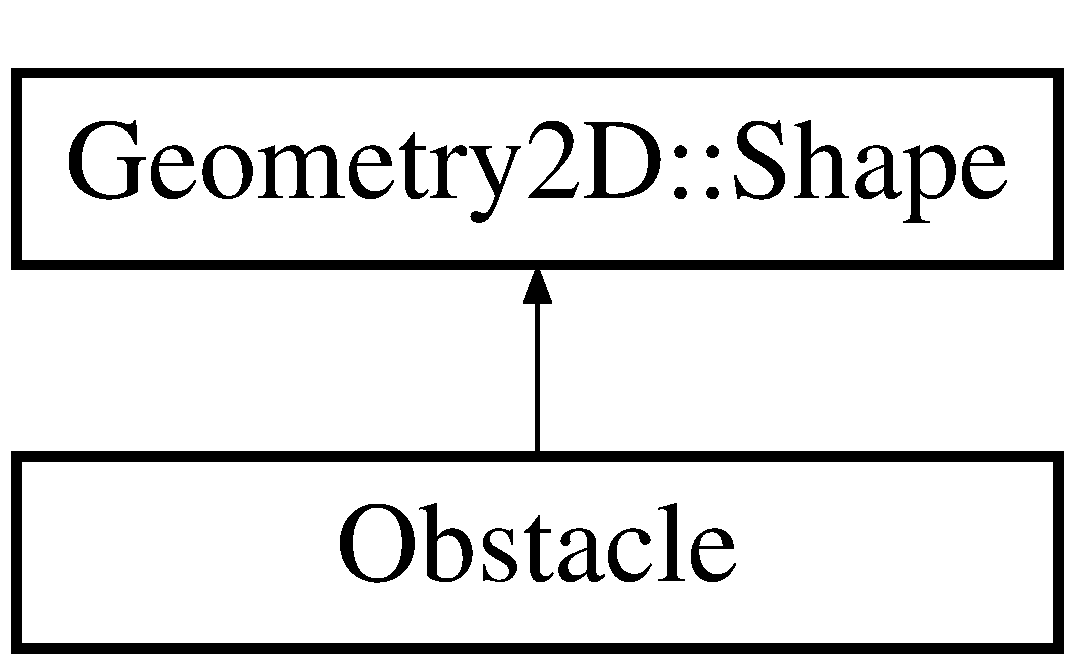
\includegraphics[height=2.000000cm]{class_obstacle}
\end{center}
\end{figure}
\subsection*{Public Member Functions}
\begin{DoxyCompactItemize}
\item 
\mbox{\hyperlink{class_obstacle_a8f734072321fa06a7b7dae2d5f50f352}{Obstacle}} ()
\item 
\mbox{\hyperlink{class_obstacle_af2f9cc9c6cff75dca0974fd5ac4f71a9}{$\sim$\+Obstacle}} ()
\item 
void \mbox{\hyperlink{class_obstacle_ae333b23b742b38e50be13bc7aec2da5b}{find\+Obstacles}} (const Mat \&img)
\item 
std\+::vector$<$ \mbox{\hyperlink{class_geometry2_d_1_1_triangle}{Triangle}} $\ast$ $>$ \mbox{\hyperlink{class_obstacle_ae4541d52e558b0995203e99d09d4d5d6}{get\+Triangles}} ()
\item 
std\+::vector$<$ \mbox{\hyperlink{class_geometry2_d_1_1_square}{Square}} $\ast$ $>$ \mbox{\hyperlink{class_obstacle_aa7d4a88d87f53bc8ba1e2b9123354f3c}{get\+Squares}} ()
\item 
std\+::vector$<$ \mbox{\hyperlink{class_geometry2_d_1_1_pentagon}{Pentagon}} $\ast$ $>$ \mbox{\hyperlink{class_obstacle_a7cbf1671e8fef324fe113517094f8428}{get\+Pentagons}} ()
\item 
std\+::vector$<$ \mbox{\hyperlink{class_geometry2_d_1_1_hexagon}{Hexagon}} $\ast$ $>$ \mbox{\hyperlink{class_obstacle_a26db0857f78a85a975957720eeb0464d}{get\+Hexagons}} ()
\end{DoxyCompactItemize}


\subsection{Detailed Description}
class for handling obstacles in the map 

\subsection{Constructor \& Destructor Documentation}
\mbox{\Hypertarget{class_obstacle_a8f734072321fa06a7b7dae2d5f50f352}\label{class_obstacle_a8f734072321fa06a7b7dae2d5f50f352}} 
\index{Obstacle@{Obstacle}!Obstacle@{Obstacle}}
\index{Obstacle@{Obstacle}!Obstacle@{Obstacle}}
\subsubsection{\texorpdfstring{Obstacle()}{Obstacle()}}
{\footnotesize\ttfamily Obstacle\+::\+Obstacle (\begin{DoxyParamCaption}{ }\end{DoxyParamCaption})}

contstructor of the \mbox{\hyperlink{class_obstacle}{Obstacle}} class \mbox{\Hypertarget{class_obstacle_af2f9cc9c6cff75dca0974fd5ac4f71a9}\label{class_obstacle_af2f9cc9c6cff75dca0974fd5ac4f71a9}} 
\index{Obstacle@{Obstacle}!````~Obstacle@{$\sim$\+Obstacle}}
\index{````~Obstacle@{$\sim$\+Obstacle}!Obstacle@{Obstacle}}
\subsubsection{\texorpdfstring{$\sim$\+Obstacle()}{~Obstacle()}}
{\footnotesize\ttfamily Obstacle\+::$\sim$\+Obstacle (\begin{DoxyParamCaption}{ }\end{DoxyParamCaption})}

destructor of the \mbox{\hyperlink{class_obstacle}{Obstacle}} class 

\subsection{Member Function Documentation}
\mbox{\Hypertarget{class_obstacle_ae333b23b742b38e50be13bc7aec2da5b}\label{class_obstacle_ae333b23b742b38e50be13bc7aec2da5b}} 
\index{Obstacle@{Obstacle}!find\+Obstacles@{find\+Obstacles}}
\index{find\+Obstacles@{find\+Obstacles}!Obstacle@{Obstacle}}
\subsubsection{\texorpdfstring{find\+Obstacles()}{findObstacles()}}
{\footnotesize\ttfamily void Obstacle\+::find\+Obstacles (\begin{DoxyParamCaption}\item[{const Mat \&}]{img }\end{DoxyParamCaption})}

retrieve the obstacles given a photo of the map 
\begin{DoxyParams}{Parameters}
{\em img} & \\
\hline
\end{DoxyParams}
\mbox{\Hypertarget{class_obstacle_a26db0857f78a85a975957720eeb0464d}\label{class_obstacle_a26db0857f78a85a975957720eeb0464d}} 
\index{Obstacle@{Obstacle}!get\+Hexagons@{get\+Hexagons}}
\index{get\+Hexagons@{get\+Hexagons}!Obstacle@{Obstacle}}
\subsubsection{\texorpdfstring{get\+Hexagons()}{getHexagons()}}
{\footnotesize\ttfamily std\+::vector$<$\mbox{\hyperlink{class_geometry2_d_1_1_hexagon}{Hexagon}} $\ast$$>$ Obstacle\+::get\+Hexagons (\begin{DoxyParamCaption}{ }\end{DoxyParamCaption})}

return the list of the hexagons obstacles \begin{DoxyReturn}{Returns}
list of the hexagons obstacles 
\end{DoxyReturn}
\mbox{\Hypertarget{class_obstacle_a7cbf1671e8fef324fe113517094f8428}\label{class_obstacle_a7cbf1671e8fef324fe113517094f8428}} 
\index{Obstacle@{Obstacle}!get\+Pentagons@{get\+Pentagons}}
\index{get\+Pentagons@{get\+Pentagons}!Obstacle@{Obstacle}}
\subsubsection{\texorpdfstring{get\+Pentagons()}{getPentagons()}}
{\footnotesize\ttfamily std\+::vector$<$\mbox{\hyperlink{class_geometry2_d_1_1_pentagon}{Pentagon}} $\ast$$>$ Obstacle\+::get\+Pentagons (\begin{DoxyParamCaption}{ }\end{DoxyParamCaption})}

return the list of the pentagons obstacles \begin{DoxyReturn}{Returns}
list of the pentagons obstacles 
\end{DoxyReturn}
\mbox{\Hypertarget{class_obstacle_aa7d4a88d87f53bc8ba1e2b9123354f3c}\label{class_obstacle_aa7d4a88d87f53bc8ba1e2b9123354f3c}} 
\index{Obstacle@{Obstacle}!get\+Squares@{get\+Squares}}
\index{get\+Squares@{get\+Squares}!Obstacle@{Obstacle}}
\subsubsection{\texorpdfstring{get\+Squares()}{getSquares()}}
{\footnotesize\ttfamily std\+::vector$<$\mbox{\hyperlink{class_geometry2_d_1_1_square}{Square}} $\ast$$>$ Obstacle\+::get\+Squares (\begin{DoxyParamCaption}{ }\end{DoxyParamCaption})}

return the list of the squares obstacles \begin{DoxyReturn}{Returns}
list of the squares obstacles 
\end{DoxyReturn}
\mbox{\Hypertarget{class_obstacle_ae4541d52e558b0995203e99d09d4d5d6}\label{class_obstacle_ae4541d52e558b0995203e99d09d4d5d6}} 
\index{Obstacle@{Obstacle}!get\+Triangles@{get\+Triangles}}
\index{get\+Triangles@{get\+Triangles}!Obstacle@{Obstacle}}
\subsubsection{\texorpdfstring{get\+Triangles()}{getTriangles()}}
{\footnotesize\ttfamily std\+::vector$<$\mbox{\hyperlink{class_geometry2_d_1_1_triangle}{Triangle}} $\ast$$>$ Obstacle\+::get\+Triangles (\begin{DoxyParamCaption}{ }\end{DoxyParamCaption})}

return the list of the triangles obstacles \begin{DoxyReturn}{Returns}
list of the triangles obstacles 
\end{DoxyReturn}


The documentation for this class was generated from the following file\+:\begin{DoxyCompactItemize}
\item 
Obstacle.\+hpp\end{DoxyCompactItemize}

\hypertarget{class_optical___character___recognition}{}\section{Optical\+\_\+\+Character\+\_\+\+Recognition Class Reference}
\label{class_optical___character___recognition}\index{Optical\+\_\+\+Character\+\_\+\+Recognition@{Optical\+\_\+\+Character\+\_\+\+Recognition}}


O\+CP algorithm from tesseract library.  




{\ttfamily \#include $<$Optical\+\_\+\+Character\+\_\+\+Recognition.\+hpp$>$}

Inheritance diagram for Optical\+\_\+\+Character\+\_\+\+Recognition\+:\begin{figure}[H]
\begin{center}
\leavevmode
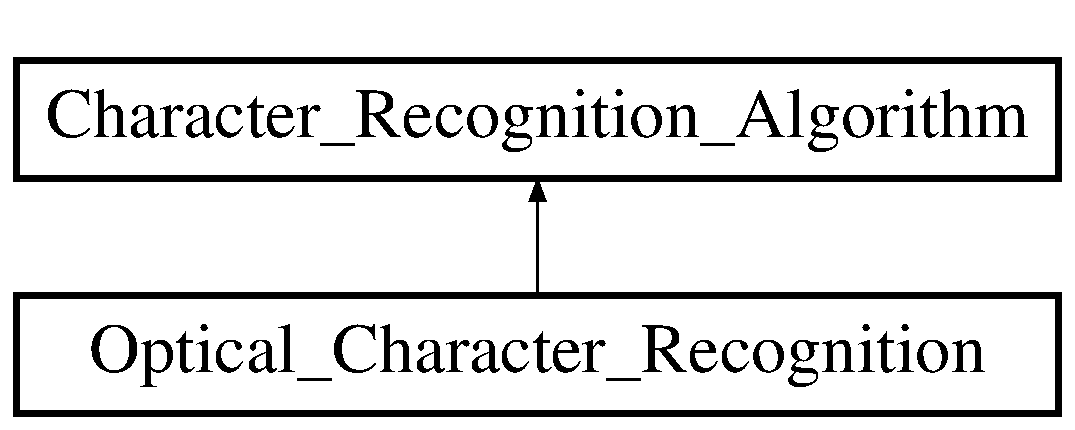
\includegraphics[height=2.000000cm]{class_optical___character___recognition}
\end{center}
\end{figure}
\subsection*{Public Member Functions}
\begin{DoxyCompactItemize}
\item 
\mbox{\Hypertarget{class_optical___character___recognition_ac94cc464313af1a3ad1c66a508826844}\label{class_optical___character___recognition_ac94cc464313af1a3ad1c66a508826844}} 
void \mbox{\hyperlink{class_optical___character___recognition_ac94cc464313af1a3ad1c66a508826844}{process\+Image}} (const std\+::string \&filename)
\begin{DoxyCompactList}\small\item\em demo function for displaying performance of algorithm \end{DoxyCompactList}\item 
\mbox{\Hypertarget{class_optical___character___recognition_a46af55e1f0a92cc025b8fdc5a48be671}\label{class_optical___character___recognition_a46af55e1f0a92cc025b8fdc5a48be671}} 
int \mbox{\hyperlink{class_optical___character___recognition_a46af55e1f0a92cc025b8fdc5a48be671}{detect\+\_\+digit}} (cv\+::\+Mat \&image, cv\+::\+Rect \&rect, cv\+::\+Mat \&R\+OI)
\begin{DoxyCompactList}\small\item\em the (virtual) function that runs the recognition engine \end{DoxyCompactList}\item 
\mbox{\Hypertarget{class_optical___character___recognition_a7bd6b6526dd287611d8bf1cd3a157796}\label{class_optical___character___recognition_a7bd6b6526dd287611d8bf1cd3a157796}} 
int {\bfseries detect\+\_\+digit} (tesseract\+::\+Tess\+Base\+A\+PI $\ast$\&O\+CR, cv\+::\+Mat \&image, cv\+::\+Rect \&rect, cv\+::\+Mat \&R\+OI)
\item 
\mbox{\Hypertarget{class_optical___character___recognition_a206d7717fa04e0b46564f56fe0c27479}\label{class_optical___character___recognition_a206d7717fa04e0b46564f56fe0c27479}} 
void {\bfseries get\+Result} (tesseract\+::\+Tess\+Base\+A\+PI $\ast$\&ocr, cv\+::\+Mat \&img, int \&result)
\item 
\mbox{\Hypertarget{class_optical___character___recognition_a011e000a7288f133cdf99cee0c31657a}\label{class_optical___character___recognition_a011e000a7288f133cdf99cee0c31657a}} 
std\+::vector$<$ std\+::pair$<$ int, cv\+::\+Rect $>$ $>$ {\bfseries detection\+\_\+algorithm} (std\+::vector$<$ cv\+::\+Rect $>$ \&bound\+Rect, cv\+::\+Mat \&filtered)
\end{DoxyCompactItemize}
\subsection*{Public Attributes}
\begin{DoxyCompactItemize}
\item 
\mbox{\Hypertarget{class_optical___character___recognition_aa23b2e408dcd91e50176fb71ae38fc96}\label{class_optical___character___recognition_aa23b2e408dcd91e50176fb71ae38fc96}} 
int {\bfseries max\+Conf} = 80
\item 
\mbox{\Hypertarget{class_optical___character___recognition_ad3fdb2f00dd03892c0e25ace9795ed42}\label{class_optical___character___recognition_ad3fdb2f00dd03892c0e25ace9795ed42}} 
tesseract\+::\+Tess\+Base\+A\+PI $\ast$ {\bfseries ocr} = new tesseract\+::\+Tess\+Base\+A\+PI()
\end{DoxyCompactItemize}


\subsection{Detailed Description}
O\+CP algorithm from tesseract library. 

The documentation for this class was generated from the following file\+:\begin{DoxyCompactItemize}
\item 
Optical\+\_\+\+Character\+\_\+\+Recognition.\+hpp\end{DoxyCompactItemize}

\hypertarget{class_path}{}\section{Path Class Reference}
\label{class_path}\index{Path@{Path}}
\subsection*{Public Member Functions}
\begin{DoxyCompactItemize}
\item 
\mbox{\hyperlink{class_path_a6abfa12b45ae127daa7408571b62b74d}{Path}} (\mbox{\hyperlink{class_position}{Position}} start\+\_\+point, \mbox{\hyperlink{class_position}{Position}} end\+\_\+point, double curvature, \mbox{\hyperlink{class_map}{Map}} $\ast$map\+\_\+i)
\begin{DoxyCompactList}\small\item\em given the start point and the end point is able to find the best path \end{DoxyCompactList}\item 
\mbox{\Hypertarget{class_path_ab45faf702862c6594068a3ed2d026cda}\label{class_path_ab45faf702862c6594068a3ed2d026cda}} 
void \mbox{\hyperlink{class_path_ab45faf702862c6594068a3ed2d026cda}{find\+Path}} ()
\begin{DoxyCompactList}\small\item\em function that detects the best path, for now uses only dubins path \end{DoxyCompactList}\item 
\mbox{\Hypertarget{class_path_ae5b5816b3480e9f103079bb3467dc65f}\label{class_path_ae5b5816b3480e9f103079bb3467dc65f}} 
void \mbox{\hyperlink{class_path_ae5b5816b3480e9f103079bb3467dc65f}{set\+Lines}} (std\+::vector$<$ \mbox{\hyperlink{class_line}{Line}} $>$)
\begin{DoxyCompactList}\small\item\em set the lines of the path \end{DoxyCompactList}\item 
std\+::vector$<$ \mbox{\hyperlink{class_line}{Line}} $>$ \mbox{\hyperlink{class_path_aff0072e2e1cf183ba6fc240cd85045e2}{get\+Lines}} ()
\begin{DoxyCompactList}\small\item\em return a vector of lines \end{DoxyCompactList}\item 
void \mbox{\hyperlink{class_path_a87f4082a3c5af3aa37260cb99c605156}{set\+Start\+Point}} (\mbox{\hyperlink{class_position}{Position}} start\+\_\+point)
\begin{DoxyCompactList}\small\item\em set the start point of the path \end{DoxyCompactList}\item 
\mbox{\hyperlink{class_position}{Position}} \mbox{\hyperlink{class_path_a88e537e6bfe6140d00b0f36ca642a4cd}{get\+Start\+Point}} ()
\begin{DoxyCompactList}\small\item\em return the start point of the path \end{DoxyCompactList}\item 
void \mbox{\hyperlink{class_path_a168f515818fd9b26a6264fdf95af52e8}{set\+End\+Point}} (\mbox{\hyperlink{class_position}{Position}} end\+\_\+point)
\begin{DoxyCompactList}\small\item\em set the end point of the path \end{DoxyCompactList}\item 
\mbox{\hyperlink{class_position}{Position}} \mbox{\hyperlink{class_path_ac2617080c944b93f7c0c63f3e59aa88c}{get\+End\+Point}} ()
\begin{DoxyCompactList}\small\item\em return the end point of the path \end{DoxyCompactList}\item 
void \mbox{\hyperlink{class_path_a132d54dc6350d1c2eb86611db60df7ff}{set\+Max\+Curvature}} (double curvature)
\begin{DoxyCompactList}\small\item\em set max curvature of the path \end{DoxyCompactList}\item 
double \mbox{\hyperlink{class_path_a613552d171c766462f422593b4957ecc}{get\+Max\+Curvature}} ()
\begin{DoxyCompactList}\small\item\em return of max curvature of the path \end{DoxyCompactList}\item 
void \mbox{\hyperlink{class_path_ad723ba990a07d7542703770a09df52a7}{set\+Length}} (double length)
\begin{DoxyCompactList}\small\item\em set the length of the path \end{DoxyCompactList}\item 
double \mbox{\hyperlink{class_path_ad497d2a12a47bc52a316da83dbe6acbc}{get\+Length}} ()
\begin{DoxyCompactList}\small\item\em return the length of the path \end{DoxyCompactList}\item 
\mbox{\Hypertarget{class_path_a68a50ad6f0fd39d0b272bcb62655b475}\label{class_path_a68a50ad6f0fd39d0b272bcb62655b475}} 
void {\bfseries set\+Map} (\mbox{\hyperlink{class_map}{Map}} $\ast$map\+\_\+i)
\item 
\mbox{\Hypertarget{class_path_abacf46c32c4f36a79c2faf21a9a01270}\label{class_path_abacf46c32c4f36a79c2faf21a9a01270}} 
\mbox{\hyperlink{class_map}{Map}} $\ast$ {\bfseries get\+Map} ()
\end{DoxyCompactItemize}
\subsection*{Public Attributes}
\begin{DoxyCompactItemize}
\item 
\mbox{\Hypertarget{class_path_a822c83d45ed5e336376a813c806ff66b}\label{class_path_a822c83d45ed5e336376a813c806ff66b}} 
\mbox{\hyperlink{class_position}{Position}} {\bfseries start\+\_\+point}
\item 
\mbox{\Hypertarget{class_path_ab97cd4eb2fa1141118bd561c824b27cc}\label{class_path_ab97cd4eb2fa1141118bd561c824b27cc}} 
\mbox{\hyperlink{class_position}{Position}} {\bfseries end\+\_\+point}
\item 
\mbox{\Hypertarget{class_path_a181a2058e947c22fc3e25a361bb934e6}\label{class_path_a181a2058e947c22fc3e25a361bb934e6}} 
double {\bfseries max\+Curvature}
\item 
\mbox{\Hypertarget{class_path_a3d38eb2e010fbf82837e7d3eb5f0faba}\label{class_path_a3d38eb2e010fbf82837e7d3eb5f0faba}} 
std\+::vector$<$ \mbox{\hyperlink{class_line}{Line}} $>$ {\bfseries lines}
\item 
\mbox{\Hypertarget{class_path_a8ca4f648459940bdd347e52f07676473}\label{class_path_a8ca4f648459940bdd347e52f07676473}} 
double {\bfseries length}
\item 
\mbox{\Hypertarget{class_path_a13645419b6b5876ce59368184742b8d7}\label{class_path_a13645419b6b5876ce59368184742b8d7}} 
\mbox{\hyperlink{class_map}{Map}} $\ast$ {\bfseries map}
\end{DoxyCompactItemize}


\subsection{Constructor \& Destructor Documentation}
\mbox{\Hypertarget{class_path_a6abfa12b45ae127daa7408571b62b74d}\label{class_path_a6abfa12b45ae127daa7408571b62b74d}} 
\index{Path@{Path}!Path@{Path}}
\index{Path@{Path}!Path@{Path}}
\subsubsection{\texorpdfstring{Path()}{Path()}}
{\footnotesize\ttfamily Path\+::\+Path (\begin{DoxyParamCaption}\item[{\mbox{\hyperlink{class_position}{Position}}}]{start\+\_\+point,  }\item[{\mbox{\hyperlink{class_position}{Position}}}]{end\+\_\+point,  }\item[{double}]{curvature,  }\item[{\mbox{\hyperlink{class_map}{Map}} $\ast$}]{map\+\_\+i }\end{DoxyParamCaption})}



given the start point and the end point is able to find the best path 


\begin{DoxyParams}{Parameters}
{\em start\+\_\+point} & start point \\
\hline
{\em end\+\_\+point} & end point \\
\hline
\end{DoxyParams}


\subsection{Member Function Documentation}
\mbox{\Hypertarget{class_path_ac2617080c944b93f7c0c63f3e59aa88c}\label{class_path_ac2617080c944b93f7c0c63f3e59aa88c}} 
\index{Path@{Path}!get\+End\+Point@{get\+End\+Point}}
\index{get\+End\+Point@{get\+End\+Point}!Path@{Path}}
\subsubsection{\texorpdfstring{get\+End\+Point()}{getEndPoint()}}
{\footnotesize\ttfamily \mbox{\hyperlink{class_position}{Position}} Path\+::get\+End\+Point (\begin{DoxyParamCaption}{ }\end{DoxyParamCaption})}



return the end point of the path 

\begin{DoxyReturn}{Returns}
the end point of the path 
\end{DoxyReturn}
\mbox{\Hypertarget{class_path_ad497d2a12a47bc52a316da83dbe6acbc}\label{class_path_ad497d2a12a47bc52a316da83dbe6acbc}} 
\index{Path@{Path}!get\+Length@{get\+Length}}
\index{get\+Length@{get\+Length}!Path@{Path}}
\subsubsection{\texorpdfstring{get\+Length()}{getLength()}}
{\footnotesize\ttfamily double Path\+::get\+Length (\begin{DoxyParamCaption}{ }\end{DoxyParamCaption})}



return the length of the path 

\begin{DoxyReturn}{Returns}
the length 

the length 
\end{DoxyReturn}
\mbox{\Hypertarget{class_path_aff0072e2e1cf183ba6fc240cd85045e2}\label{class_path_aff0072e2e1cf183ba6fc240cd85045e2}} 
\index{Path@{Path}!get\+Lines@{get\+Lines}}
\index{get\+Lines@{get\+Lines}!Path@{Path}}
\subsubsection{\texorpdfstring{get\+Lines()}{getLines()}}
{\footnotesize\ttfamily std\+::vector$<$\mbox{\hyperlink{class_line}{Line}}$>$ Path\+::get\+Lines (\begin{DoxyParamCaption}{ }\end{DoxyParamCaption})}



return a vector of lines 

\begin{DoxyReturn}{Returns}
vector of lines 
\end{DoxyReturn}
\mbox{\Hypertarget{class_path_a613552d171c766462f422593b4957ecc}\label{class_path_a613552d171c766462f422593b4957ecc}} 
\index{Path@{Path}!get\+Max\+Curvature@{get\+Max\+Curvature}}
\index{get\+Max\+Curvature@{get\+Max\+Curvature}!Path@{Path}}
\subsubsection{\texorpdfstring{get\+Max\+Curvature()}{getMaxCurvature()}}
{\footnotesize\ttfamily double Path\+::get\+Max\+Curvature (\begin{DoxyParamCaption}{ }\end{DoxyParamCaption})}



return of max curvature of the path 

\begin{DoxyReturn}{Returns}
the max curvature of the path 
\end{DoxyReturn}
\mbox{\Hypertarget{class_path_a88e537e6bfe6140d00b0f36ca642a4cd}\label{class_path_a88e537e6bfe6140d00b0f36ca642a4cd}} 
\index{Path@{Path}!get\+Start\+Point@{get\+Start\+Point}}
\index{get\+Start\+Point@{get\+Start\+Point}!Path@{Path}}
\subsubsection{\texorpdfstring{get\+Start\+Point()}{getStartPoint()}}
{\footnotesize\ttfamily \mbox{\hyperlink{class_position}{Position}} Path\+::get\+Start\+Point (\begin{DoxyParamCaption}{ }\end{DoxyParamCaption})}



return the start point of the path 

\begin{DoxyReturn}{Returns}
the start point of the path 
\end{DoxyReturn}
\mbox{\Hypertarget{class_path_a168f515818fd9b26a6264fdf95af52e8}\label{class_path_a168f515818fd9b26a6264fdf95af52e8}} 
\index{Path@{Path}!set\+End\+Point@{set\+End\+Point}}
\index{set\+End\+Point@{set\+End\+Point}!Path@{Path}}
\subsubsection{\texorpdfstring{set\+End\+Point()}{setEndPoint()}}
{\footnotesize\ttfamily void Path\+::set\+End\+Point (\begin{DoxyParamCaption}\item[{\mbox{\hyperlink{class_position}{Position}}}]{end\+\_\+point }\end{DoxyParamCaption})}



set the end point of the path 


\begin{DoxyParams}{Parameters}
{\em end\+\_\+point} & the end point of the path \\
\hline
\end{DoxyParams}
\mbox{\Hypertarget{class_path_ad723ba990a07d7542703770a09df52a7}\label{class_path_ad723ba990a07d7542703770a09df52a7}} 
\index{Path@{Path}!set\+Length@{set\+Length}}
\index{set\+Length@{set\+Length}!Path@{Path}}
\subsubsection{\texorpdfstring{set\+Length()}{setLength()}}
{\footnotesize\ttfamily void Path\+::set\+Length (\begin{DoxyParamCaption}\item[{double}]{length }\end{DoxyParamCaption})}



set the length of the path 


\begin{DoxyParams}{Parameters}
{\em length} & length of the path \\
\hline
\end{DoxyParams}
\mbox{\Hypertarget{class_path_a132d54dc6350d1c2eb86611db60df7ff}\label{class_path_a132d54dc6350d1c2eb86611db60df7ff}} 
\index{Path@{Path}!set\+Max\+Curvature@{set\+Max\+Curvature}}
\index{set\+Max\+Curvature@{set\+Max\+Curvature}!Path@{Path}}
\subsubsection{\texorpdfstring{set\+Max\+Curvature()}{setMaxCurvature()}}
{\footnotesize\ttfamily void Path\+::set\+Max\+Curvature (\begin{DoxyParamCaption}\item[{double}]{curvature }\end{DoxyParamCaption})}



set max curvature of the path 


\begin{DoxyParams}{Parameters}
{\em curvature} & max curvature of the path \\
\hline
\end{DoxyParams}
\mbox{\Hypertarget{class_path_a87f4082a3c5af3aa37260cb99c605156}\label{class_path_a87f4082a3c5af3aa37260cb99c605156}} 
\index{Path@{Path}!set\+Start\+Point@{set\+Start\+Point}}
\index{set\+Start\+Point@{set\+Start\+Point}!Path@{Path}}
\subsubsection{\texorpdfstring{set\+Start\+Point()}{setStartPoint()}}
{\footnotesize\ttfamily void Path\+::set\+Start\+Point (\begin{DoxyParamCaption}\item[{\mbox{\hyperlink{class_position}{Position}}}]{start\+\_\+point }\end{DoxyParamCaption})}



set the start point of the path 


\begin{DoxyParams}{Parameters}
{\em start\+\_\+point} & start point of the path \\
\hline
\end{DoxyParams}


The documentation for this class was generated from the following file\+:\begin{DoxyCompactItemize}
\item 
Path.\+hpp\end{DoxyCompactItemize}

\hypertarget{class_path_coordinates}{}\section{Path\+Coordinates Class Reference}
\label{class_path_coordinates}\index{Path\+Coordinates@{Path\+Coordinates}}


class for storing data that describes the path  




{\ttfamily \#include $<$Path\+Coordinates.\+hpp$>$}

\subsection*{Public Member Functions}
\begin{DoxyCompactItemize}
\item 
\mbox{\hyperlink{class_path_coordinates_a6540a40d24cb4e50577eda489b7fe1bb}{Path\+Coordinates}} (\mbox{\hyperlink{class_position}{Position}} position\+\_\+in, \mbox{\hyperlink{class_position}{Position}} position\+\_\+fin, double curvature\+\_\+p)
\begin{DoxyCompactList}\small\item\em constructor of the \mbox{\hyperlink{class_path_coordinates}{Path\+Coordinates}} class \end{DoxyCompactList}\item 
\mbox{\Hypertarget{class_path_coordinates_a960c365c8307fb139e425a24d2eb8c66}\label{class_path_coordinates_a960c365c8307fb139e425a24d2eb8c66}} 
\mbox{\hyperlink{class_path_coordinates_a960c365c8307fb139e425a24d2eb8c66}{$\sim$\+Path\+Coordinates}} ()
\begin{DoxyCompactList}\small\item\em destructor of the \mbox{\hyperlink{class_path_coordinates}{Path\+Coordinates}} class \end{DoxyCompactList}\item 
void \mbox{\hyperlink{class_path_coordinates_a730ba85010cbd33da4e76fe0f05fb2b0}{set\+Positions}} (\mbox{\hyperlink{class_position}{Position}} position\+\_\+in, \mbox{\hyperlink{class_position}{Position}} position\+\_\+fin)
\item 
\mbox{\hyperlink{class_position}{Position}} \mbox{\hyperlink{class_path_coordinates_a10450bb899bec6d9f8be0a115c2c588b}{get\+Initial\+Position}} ()
\begin{DoxyCompactList}\small\item\em return the initial position of the path \end{DoxyCompactList}\item 
\mbox{\hyperlink{class_position}{Position}} \mbox{\hyperlink{class_path_coordinates_af4d85fae7c4ed67ea5201895d1ee4b7b}{get\+Final\+Position}} ()
\begin{DoxyCompactList}\small\item\em return the final position of the path \end{DoxyCompactList}\item 
double \mbox{\hyperlink{class_path_coordinates_a6b0315b737b35af2e198a7094828741e}{get\+Max\+Curvature}} ()
\begin{DoxyCompactList}\small\item\em return the curvature of the path \end{DoxyCompactList}\item 
void \mbox{\hyperlink{class_path_coordinates_abd7e9a8143e368f9290b962f595ae0a8}{set\+Max\+Curvature}} (double curvature\+\_\+p)
\begin{DoxyCompactList}\small\item\em set the max curvature of the path \end{DoxyCompactList}\end{DoxyCompactItemize}


\subsection{Detailed Description}
class for storing data that describes the path 

\subsection{Constructor \& Destructor Documentation}
\mbox{\Hypertarget{class_path_coordinates_a6540a40d24cb4e50577eda489b7fe1bb}\label{class_path_coordinates_a6540a40d24cb4e50577eda489b7fe1bb}} 
\index{Path\+Coordinates@{Path\+Coordinates}!Path\+Coordinates@{Path\+Coordinates}}
\index{Path\+Coordinates@{Path\+Coordinates}!Path\+Coordinates@{Path\+Coordinates}}
\subsubsection{\texorpdfstring{Path\+Coordinates()}{PathCoordinates()}}
{\footnotesize\ttfamily Path\+Coordinates\+::\+Path\+Coordinates (\begin{DoxyParamCaption}\item[{\mbox{\hyperlink{class_position}{Position}}}]{position\+\_\+in,  }\item[{\mbox{\hyperlink{class_position}{Position}}}]{position\+\_\+fin,  }\item[{double}]{curvature\+\_\+p }\end{DoxyParamCaption})}



constructor of the \mbox{\hyperlink{class_path_coordinates}{Path\+Coordinates}} class 


\begin{DoxyParams}{Parameters}
{\em position\+\_\+in} & initial position of the path \\
\hline
{\em position\+\_\+fin} & final position if the path \\
\hline
{\em curvature\+\_\+p} & curvature of the path \\
\hline
\end{DoxyParams}


\subsection{Member Function Documentation}
\mbox{\Hypertarget{class_path_coordinates_af4d85fae7c4ed67ea5201895d1ee4b7b}\label{class_path_coordinates_af4d85fae7c4ed67ea5201895d1ee4b7b}} 
\index{Path\+Coordinates@{Path\+Coordinates}!get\+Final\+Position@{get\+Final\+Position}}
\index{get\+Final\+Position@{get\+Final\+Position}!Path\+Coordinates@{Path\+Coordinates}}
\subsubsection{\texorpdfstring{get\+Final\+Position()}{getFinalPosition()}}
{\footnotesize\ttfamily \mbox{\hyperlink{class_position}{Position}} Path\+Coordinates\+::get\+Final\+Position (\begin{DoxyParamCaption}{ }\end{DoxyParamCaption})}



return the final position of the path 

\begin{DoxyReturn}{Returns}
the final position of the path 
\end{DoxyReturn}
\mbox{\Hypertarget{class_path_coordinates_a10450bb899bec6d9f8be0a115c2c588b}\label{class_path_coordinates_a10450bb899bec6d9f8be0a115c2c588b}} 
\index{Path\+Coordinates@{Path\+Coordinates}!get\+Initial\+Position@{get\+Initial\+Position}}
\index{get\+Initial\+Position@{get\+Initial\+Position}!Path\+Coordinates@{Path\+Coordinates}}
\subsubsection{\texorpdfstring{get\+Initial\+Position()}{getInitialPosition()}}
{\footnotesize\ttfamily \mbox{\hyperlink{class_position}{Position}} Path\+Coordinates\+::get\+Initial\+Position (\begin{DoxyParamCaption}{ }\end{DoxyParamCaption})}



return the initial position of the path 

\begin{DoxyReturn}{Returns}
the initial position of the path 
\end{DoxyReturn}
\mbox{\Hypertarget{class_path_coordinates_a6b0315b737b35af2e198a7094828741e}\label{class_path_coordinates_a6b0315b737b35af2e198a7094828741e}} 
\index{Path\+Coordinates@{Path\+Coordinates}!get\+Max\+Curvature@{get\+Max\+Curvature}}
\index{get\+Max\+Curvature@{get\+Max\+Curvature}!Path\+Coordinates@{Path\+Coordinates}}
\subsubsection{\texorpdfstring{get\+Max\+Curvature()}{getMaxCurvature()}}
{\footnotesize\ttfamily double Path\+Coordinates\+::get\+Max\+Curvature (\begin{DoxyParamCaption}{ }\end{DoxyParamCaption})}



return the curvature of the path 

\begin{DoxyReturn}{Returns}
the curvature of the path 
\end{DoxyReturn}
\mbox{\Hypertarget{class_path_coordinates_abd7e9a8143e368f9290b962f595ae0a8}\label{class_path_coordinates_abd7e9a8143e368f9290b962f595ae0a8}} 
\index{Path\+Coordinates@{Path\+Coordinates}!set\+Max\+Curvature@{set\+Max\+Curvature}}
\index{set\+Max\+Curvature@{set\+Max\+Curvature}!Path\+Coordinates@{Path\+Coordinates}}
\subsubsection{\texorpdfstring{set\+Max\+Curvature()}{setMaxCurvature()}}
{\footnotesize\ttfamily void Path\+Coordinates\+::set\+Max\+Curvature (\begin{DoxyParamCaption}\item[{double}]{curvature\+\_\+p }\end{DoxyParamCaption})}



set the max curvature of the path 


\begin{DoxyParams}{Parameters}
{\em curvature\+\_\+p} & the max curvature of the path \\
\hline
\end{DoxyParams}
\mbox{\Hypertarget{class_path_coordinates_a730ba85010cbd33da4e76fe0f05fb2b0}\label{class_path_coordinates_a730ba85010cbd33da4e76fe0f05fb2b0}} 
\index{Path\+Coordinates@{Path\+Coordinates}!set\+Positions@{set\+Positions}}
\index{set\+Positions@{set\+Positions}!Path\+Coordinates@{Path\+Coordinates}}
\subsubsection{\texorpdfstring{set\+Positions()}{setPositions()}}
{\footnotesize\ttfamily void Path\+Coordinates\+::set\+Positions (\begin{DoxyParamCaption}\item[{\mbox{\hyperlink{class_position}{Position}}}]{position\+\_\+in,  }\item[{\mbox{\hyperlink{class_position}{Position}}}]{position\+\_\+fin }\end{DoxyParamCaption})}

set the initial and the final position of the path 
\begin{DoxyParams}{Parameters}
{\em position\+\_\+in} & initial position of the path \\
\hline
{\em position\+\_\+fin} & final position of the path \\
\hline
\end{DoxyParams}


The documentation for this class was generated from the following file\+:\begin{DoxyCompactItemize}
\item 
Path\+Coordinates.\+hpp\end{DoxyCompactItemize}

\hypertarget{class_pentagon}{}\section{Pentagon Class Reference}
\label{class_pentagon}\index{Pentagon@{Pentagon}}


Class for hadling pentagon obstacles in the map.  




{\ttfamily \#include $<$Pentagon.\+hpp$>$}

Inheritance diagram for Pentagon\+:\begin{figure}[H]
\begin{center}
\leavevmode
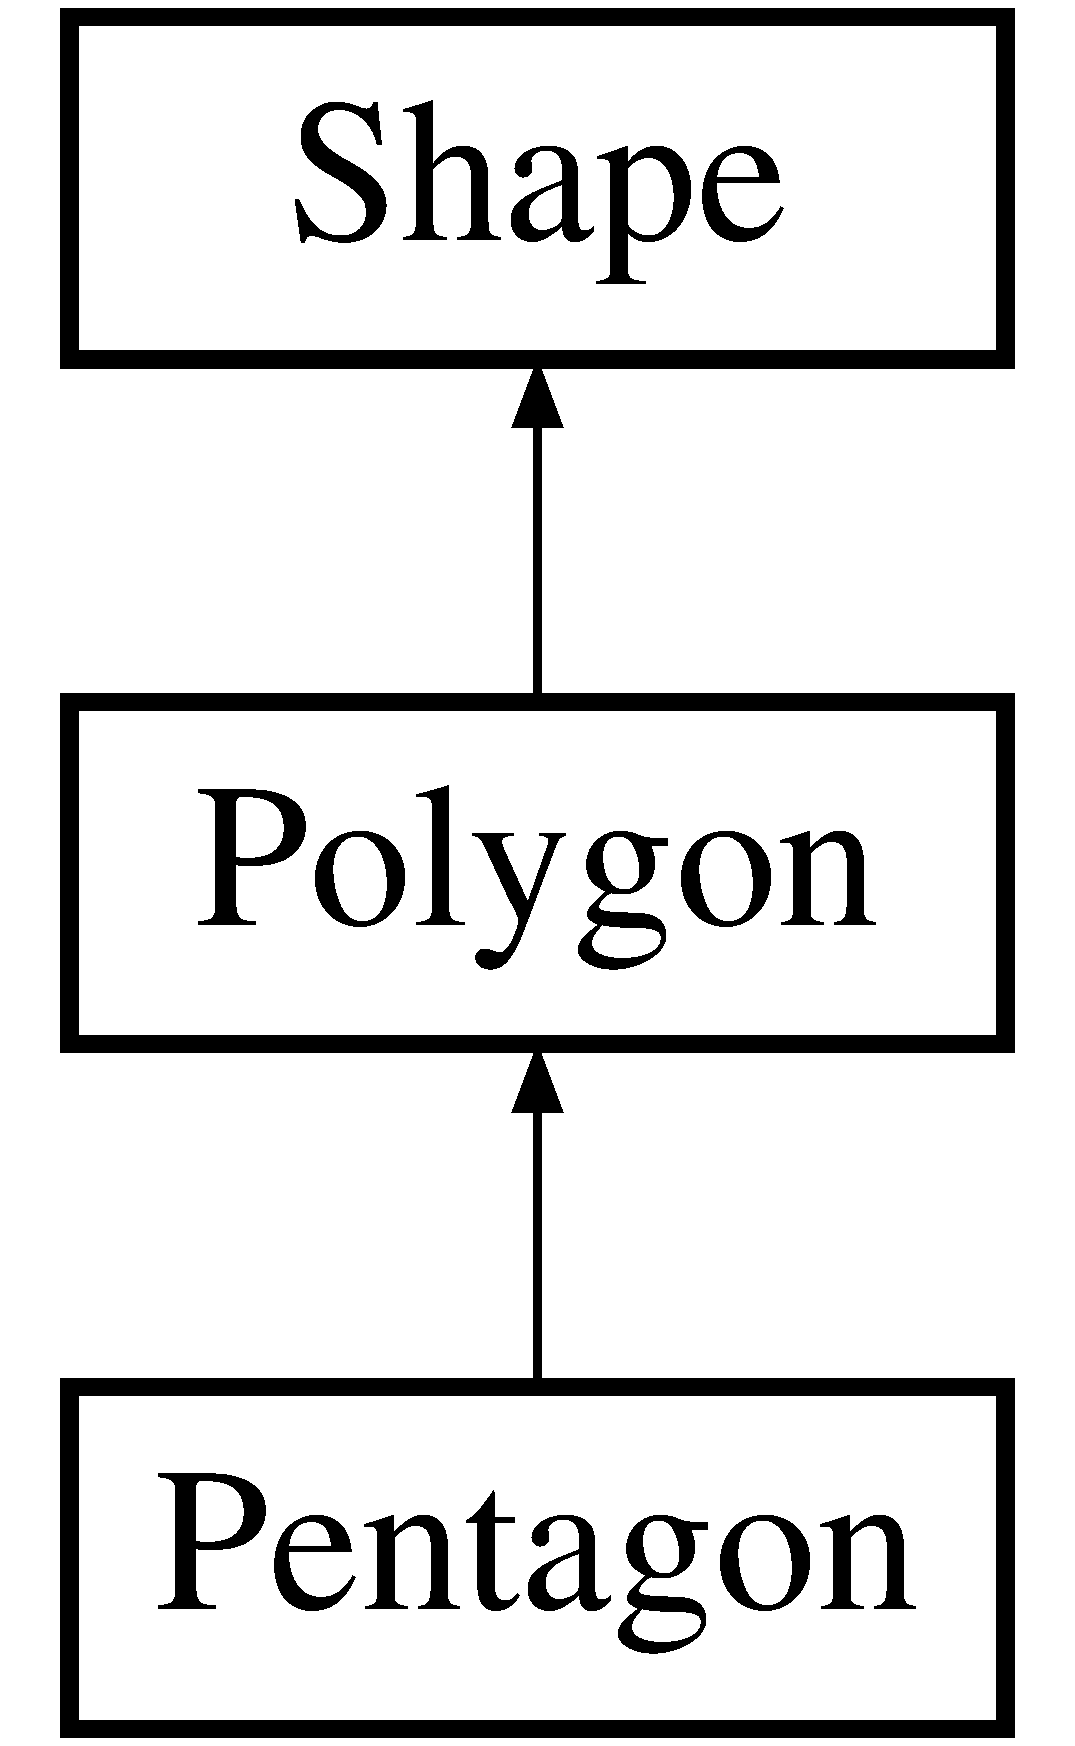
\includegraphics[height=3.000000cm]{class_pentagon}
\end{center}
\end{figure}
\subsection*{Public Member Functions}
\begin{DoxyCompactItemize}
\item 
\mbox{\hyperlink{class_pentagon_a1c5596d8ff548bfcdccc7fa53b81355c}{Pentagon}} ()
\item 
\mbox{\Hypertarget{class_pentagon_ac6d6f3dad8d75557a8f8bbf5a71d52a9}\label{class_pentagon_ac6d6f3dad8d75557a8f8bbf5a71d52a9}} 
{\bfseries Pentagon} (std\+::vector$<$ cv\+::\+Point $>$ \mbox{\hyperlink{class_polygon_a347474823f6113a34fdefeee276d1b9e}{points}})
\item 
\mbox{\hyperlink{class_pentagon_a500031431177cee506fd7f0517d84753}{$\sim$\+Pentagon}} ()
\item 
std\+::vector$<$ cv\+::\+Point $>$ \mbox{\hyperlink{class_pentagon_ab38482973f796da34cd9ac62cefb1491}{get\+Corners}} ()
\item 
void \mbox{\hyperlink{class_pentagon_a42c8df4cbb1fcf985c96c9886a21c70a}{set\+Corners}} (std\+::vector$<$ cv\+::\+Point $>$ corners)
\item 
\mbox{\Hypertarget{class_pentagon_a71ead2b4648a9772bc5be704a43df981}\label{class_pentagon_a71ead2b4648a9772bc5be704a43df981}} 
void \mbox{\hyperlink{class_pentagon_a71ead2b4648a9772bc5be704a43df981}{assign\+\_\+points}} ()
\begin{DoxyCompactList}\small\item\em assignes points to 1., 2., 3 etc point. \end{DoxyCompactList}\end{DoxyCompactItemize}
\subsection*{Additional Inherited Members}


\subsection{Detailed Description}
Class for hadling pentagon obstacles in the map. 

\subsection{Constructor \& Destructor Documentation}
\mbox{\Hypertarget{class_pentagon_a1c5596d8ff548bfcdccc7fa53b81355c}\label{class_pentagon_a1c5596d8ff548bfcdccc7fa53b81355c}} 
\index{Pentagon@{Pentagon}!Pentagon@{Pentagon}}
\index{Pentagon@{Pentagon}!Pentagon@{Pentagon}}
\subsubsection{\texorpdfstring{Pentagon()}{Pentagon()}}
{\footnotesize\ttfamily Pentagon\+::\+Pentagon (\begin{DoxyParamCaption}{ }\end{DoxyParamCaption})}

constructor of \mbox{\hyperlink{class_pentagon}{Pentagon}} class \mbox{\Hypertarget{class_pentagon_a500031431177cee506fd7f0517d84753}\label{class_pentagon_a500031431177cee506fd7f0517d84753}} 
\index{Pentagon@{Pentagon}!````~Pentagon@{$\sim$\+Pentagon}}
\index{````~Pentagon@{$\sim$\+Pentagon}!Pentagon@{Pentagon}}
\subsubsection{\texorpdfstring{$\sim$\+Pentagon()}{~Pentagon()}}
{\footnotesize\ttfamily Pentagon\+::$\sim$\+Pentagon (\begin{DoxyParamCaption}{ }\end{DoxyParamCaption})}

destructor of \mbox{\hyperlink{class_pentagon}{Pentagon}} class 

\subsection{Member Function Documentation}
\mbox{\Hypertarget{class_pentagon_ab38482973f796da34cd9ac62cefb1491}\label{class_pentagon_ab38482973f796da34cd9ac62cefb1491}} 
\index{Pentagon@{Pentagon}!get\+Corners@{get\+Corners}}
\index{get\+Corners@{get\+Corners}!Pentagon@{Pentagon}}
\subsubsection{\texorpdfstring{get\+Corners()}{getCorners()}}
{\footnotesize\ttfamily std\+::vector$<$cv\+::\+Point$>$ Pentagon\+::get\+Corners (\begin{DoxyParamCaption}{ }\end{DoxyParamCaption})}

return the list of corners of the pentagons \begin{DoxyReturn}{Returns}
the list of corners of the amaz 
\end{DoxyReturn}
\mbox{\Hypertarget{class_pentagon_a42c8df4cbb1fcf985c96c9886a21c70a}\label{class_pentagon_a42c8df4cbb1fcf985c96c9886a21c70a}} 
\index{Pentagon@{Pentagon}!set\+Corners@{set\+Corners}}
\index{set\+Corners@{set\+Corners}!Pentagon@{Pentagon}}
\subsubsection{\texorpdfstring{set\+Corners()}{setCorners()}}
{\footnotesize\ttfamily void Pentagon\+::set\+Corners (\begin{DoxyParamCaption}\item[{std\+::vector$<$ cv\+::\+Point $>$}]{corners }\end{DoxyParamCaption})}

set the corners of the pentagon 
\begin{DoxyParams}{Parameters}
{\em corners} & list of corners to be setted \\
\hline
\end{DoxyParams}


The documentation for this class was generated from the following file\+:\begin{DoxyCompactItemize}
\item 
Pentagon.\+hpp\end{DoxyCompactItemize}

\hypertarget{class_people}{}\section{People Class Reference}
\label{class_people}\index{People@{People}}


class for representing people in the map that have to be collected  




{\ttfamily \#include $<$People.\+hpp$>$}

Inheritance diagram for People\+:\begin{figure}[H]
\begin{center}
\leavevmode
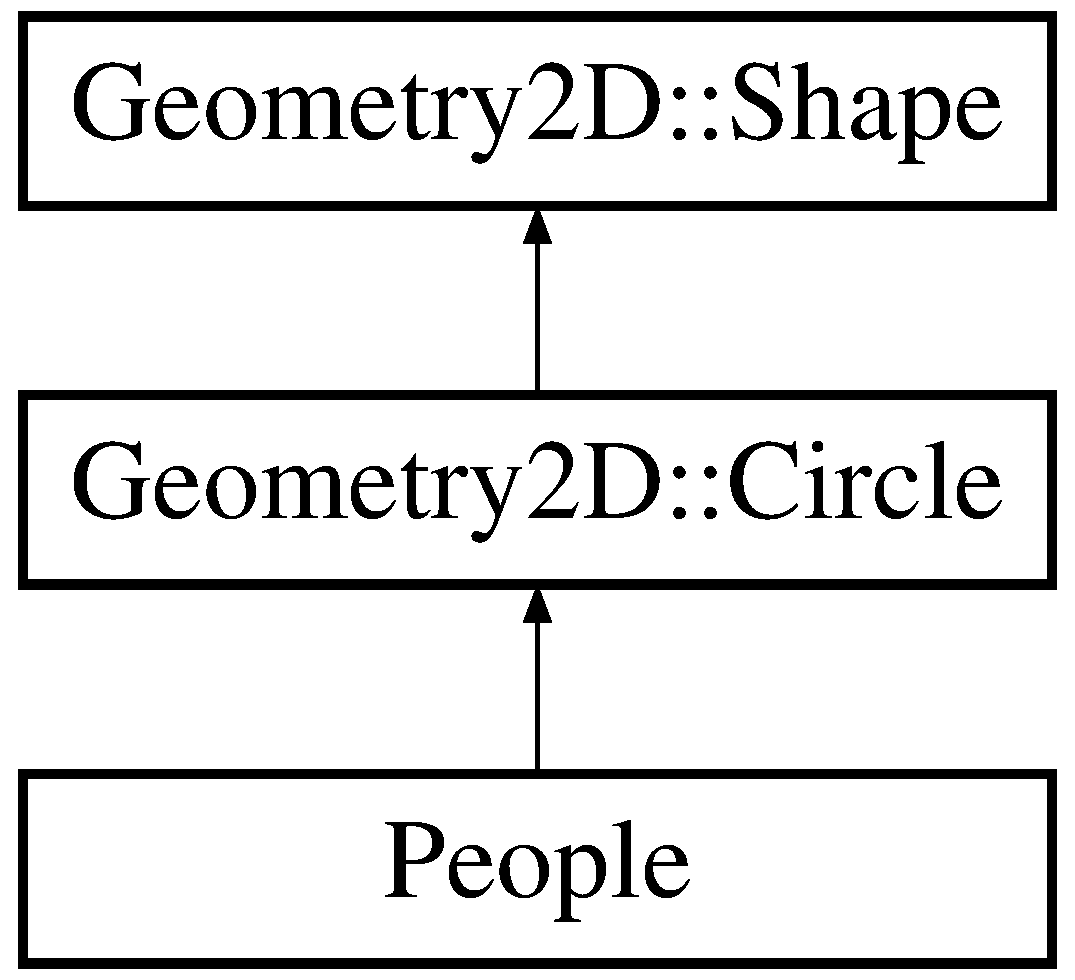
\includegraphics[height=3.000000cm]{class_people}
\end{center}
\end{figure}
\subsection*{Public Member Functions}
\begin{DoxyCompactItemize}
\item 
\mbox{\hyperlink{class_people_aae1408eddfd15a5007003ecdf1507941}{People}} ()
\item 
\mbox{\Hypertarget{class_people_abfabd2f2e27a7aa269d404e8f27f903e}\label{class_people_abfabd2f2e27a7aa269d404e8f27f903e}} 
{\bfseries People} (std\+::pair$<$ int, int $>$ digit, cv\+::\+Rect rect)
\item 
\mbox{\hyperlink{class_people_adae124857f64dadff4e1801410b3dab2}{$\sim$\+People}} ()
\end{DoxyCompactItemize}
\subsection*{Public Attributes}
\begin{DoxyCompactItemize}
\item 
\mbox{\Hypertarget{class_people_a06e995c8c3b9808db931bedb44d782c8}\label{class_people_a06e995c8c3b9808db931bedb44d782c8}} 
int \mbox{\hyperlink{class_people_a06e995c8c3b9808db931bedb44d782c8}{name}}
\begin{DoxyCompactList}\small\item\em \mbox{\hyperlink{class_people}{People}} have names -\/ represented by a digit. \end{DoxyCompactList}\item 
\mbox{\Hypertarget{class_people_a44d79c52132068763c91e308e9685e06}\label{class_people_a44d79c52132068763c91e308e9685e06}} 
int \mbox{\hyperlink{class_people_a44d79c52132068763c91e308e9685e06}{confidence}}
\begin{DoxyCompactList}\small\item\em confidence that name is the correct digit \end{DoxyCompactList}\end{DoxyCompactItemize}


\subsection{Detailed Description}
class for representing people in the map that have to be collected 

\mbox{\hyperlink{class_people}{People}} are round objects with green background that need to be collected before exiting the map. \mbox{\hyperlink{class_people}{People}} have a unique identifier given by a digit. This identifier is their name. \mbox{\hyperlink{class_people}{People}} inherit all shape characteristics of Circles, because their have circular shapes. In addition to their name and form people have a confidence level assigned to them indicating how confident the character recognition algorithm was when detecting their name. 

\subsection{Constructor \& Destructor Documentation}
\mbox{\Hypertarget{class_people_aae1408eddfd15a5007003ecdf1507941}\label{class_people_aae1408eddfd15a5007003ecdf1507941}} 
\index{People@{People}!People@{People}}
\index{People@{People}!People@{People}}
\subsubsection{\texorpdfstring{People()}{People()}}
{\footnotesize\ttfamily People\+::\+People (\begin{DoxyParamCaption}{ }\end{DoxyParamCaption})}

constructor of people class \mbox{\Hypertarget{class_people_adae124857f64dadff4e1801410b3dab2}\label{class_people_adae124857f64dadff4e1801410b3dab2}} 
\index{People@{People}!````~People@{$\sim$\+People}}
\index{````~People@{$\sim$\+People}!People@{People}}
\subsubsection{\texorpdfstring{$\sim$\+People()}{~People()}}
{\footnotesize\ttfamily People\+::$\sim$\+People (\begin{DoxyParamCaption}{ }\end{DoxyParamCaption})}

destructor of people class 

The documentation for this class was generated from the following file\+:\begin{DoxyCompactItemize}
\item 
People.\+hpp\end{DoxyCompactItemize}

\hypertarget{struct_people_storage}{}\section{People\+Storage Struct Reference}
\label{struct_people_storage}\index{People\+Storage@{People\+Storage}}


Helper object to find people in the map.  




{\ttfamily \#include $<$Digit\+\_\+\+Recognition.\+hpp$>$}

\subsection*{Public Member Functions}
\begin{DoxyCompactItemize}
\item 
\mbox{\Hypertarget{struct_people_storage_a6aa999011975c71c5dac2c011d0fba4c}\label{struct_people_storage_a6aa999011975c71c5dac2c011d0fba4c}} 
{\bfseries People\+Storage} (const Mat \&img)
\item 
void \mbox{\hyperlink{struct_people_storage_a97206f5a49064a68924059861deab436}{find\+Circles}} (const Mat \&img)
\item 
\mbox{\Hypertarget{struct_people_storage_a461a143e3b928603f383eccf65a79bdf}\label{struct_people_storage_a461a143e3b928603f383eccf65a79bdf}} 
std\+::vector$<$ \mbox{\hyperlink{class_circle}{Circle}} $\ast$ $>$ \mbox{\hyperlink{struct_people_storage_a461a143e3b928603f383eccf65a79bdf}{get\+Circles}} ()
\begin{DoxyCompactList}\small\item\em extract people information as \mbox{\hyperlink{class_circle}{Circle}} objects \end{DoxyCompactList}\end{DoxyCompactItemize}
\subsection*{Public Attributes}
\begin{DoxyCompactItemize}
\item 
\mbox{\Hypertarget{struct_people_storage_a00dd487841221f7b5094934c1409957a}\label{struct_people_storage_a00dd487841221f7b5094934c1409957a}} 
std\+::vector$<$ \mbox{\hyperlink{class_people}{People}} $>$ \mbox{\hyperlink{struct_people_storage_a00dd487841221f7b5094934c1409957a}{circles}}
\begin{DoxyCompactList}\small\item\em detected \mbox{\hyperlink{class_people}{People}} \end{DoxyCompactList}\end{DoxyCompactItemize}


\subsection{Detailed Description}
Helper object to find people in the map. 

\subsection{Member Function Documentation}
\mbox{\Hypertarget{struct_people_storage_a97206f5a49064a68924059861deab436}\label{struct_people_storage_a97206f5a49064a68924059861deab436}} 
\index{People\+Storage@{People\+Storage}!find\+Circles@{find\+Circles}}
\index{find\+Circles@{find\+Circles}!People\+Storage@{People\+Storage}}
\subsubsection{\texorpdfstring{find\+Circles()}{findCircles()}}
{\footnotesize\ttfamily void People\+Storage\+::find\+Circles (\begin{DoxyParamCaption}\item[{const Mat \&}]{img }\end{DoxyParamCaption})\hspace{0.3cm}{\ttfamily [inline]}}

detect circles in the map 
\begin{DoxyParams}{Parameters}
{\em img} & image of the map \\
\hline
\end{DoxyParams}


The documentation for this struct was generated from the following file\+:\begin{DoxyCompactItemize}
\item 
Digit\+\_\+\+Recognition.\+hpp\end{DoxyCompactItemize}

\hypertarget{class_polygon}{}\section{Polygon Class Reference}
\label{class_polygon}\index{Polygon@{Polygon}}
Inheritance diagram for Polygon\+:\begin{figure}[H]
\begin{center}
\leavevmode
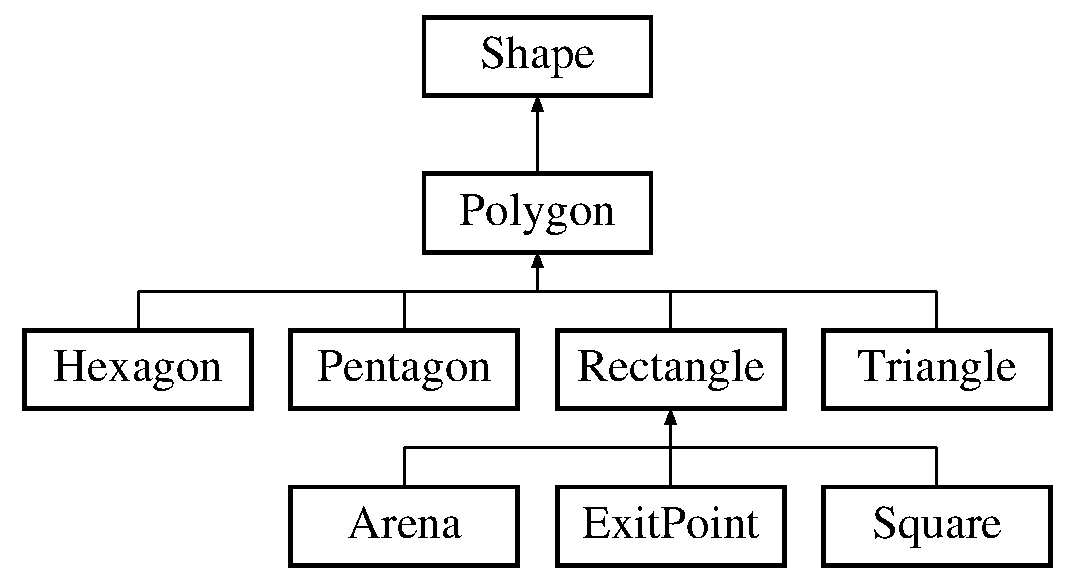
\includegraphics[height=4.000000cm]{class_polygon}
\end{center}
\end{figure}
\subsection*{Public Member Functions}
\begin{DoxyCompactItemize}
\item 
\mbox{\Hypertarget{class_polygon_ab64d7cd0303d3bf850a770a4553a03c2}\label{class_polygon_ab64d7cd0303d3bf850a770a4553a03c2}} 
{\bfseries Polygon} (std\+::vector$<$ cv\+::\+Point $>$ \mbox{\hyperlink{class_polygon_a347474823f6113a34fdefeee276d1b9e}{points}})
\item 
\mbox{\Hypertarget{class_polygon_ab2b986de126f57021357eb4bbf4d5c02}\label{class_polygon_ab2b986de126f57021357eb4bbf4d5c02}} 
virtual void \mbox{\hyperlink{class_polygon_ab2b986de126f57021357eb4bbf4d5c02}{assign\+\_\+points}} ()=0
\begin{DoxyCompactList}\small\item\em assignes the points \end{DoxyCompactList}\item 
\mbox{\Hypertarget{class_polygon_a24c56c11941cffb23b12a5cd25371578}\label{class_polygon_a24c56c11941cffb23b12a5cd25371578}} 
void {\bfseries set\+Clipped\+Corners} (std\+::vector$<$ cv\+::\+Point $>$ \&\+\_\+clipped\+\_\+corners)
\item 
\mbox{\Hypertarget{class_polygon_a675b9c01865fb77e0f6aff50e3911a28}\label{class_polygon_a675b9c01865fb77e0f6aff50e3911a28}} 
std\+::vector$<$ cv\+::\+Point $>$ {\bfseries get\+Clipped\+Corners} ()
\end{DoxyCompactItemize}
\subsection*{Public Attributes}
\begin{DoxyCompactItemize}
\item 
\mbox{\Hypertarget{class_polygon_a347474823f6113a34fdefeee276d1b9e}\label{class_polygon_a347474823f6113a34fdefeee276d1b9e}} 
std\+::vector$<$ cv\+::\+Point $>$ \mbox{\hyperlink{class_polygon_a347474823f6113a34fdefeee276d1b9e}{points}}
\begin{DoxyCompactList}\small\item\em brief the points of the polygon \end{DoxyCompactList}\item 
\mbox{\Hypertarget{class_polygon_a66cacfeac5d5f3b6852dd558abf3dc38}\label{class_polygon_a66cacfeac5d5f3b6852dd558abf3dc38}} 
std\+::vector$<$ cv\+::\+Point $>$ {\bfseries clipped\+\_\+corners}
\end{DoxyCompactItemize}


The documentation for this class was generated from the following file\+:\begin{DoxyCompactItemize}
\item 
Polygon.\+hpp\end{DoxyCompactItemize}

\hypertarget{class_position}{}\section{Position Class Reference}
\label{class_position}\index{Position@{Position}}


describes a position of a point using x and y coordinates and orientation  




{\ttfamily \#include $<$Position.\+hpp$>$}

\subsection*{Public Member Functions}
\begin{DoxyCompactItemize}
\item 
\mbox{\Hypertarget{class_position_a369a577425f8ba02e8750d04b6a088db}\label{class_position_a369a577425f8ba02e8750d04b6a088db}} 
\mbox{\hyperlink{class_position_a369a577425f8ba02e8750d04b6a088db}{Position}} ()
\begin{DoxyCompactList}\small\item\em constructor of the \mbox{\hyperlink{class_position}{Position}} class \end{DoxyCompactList}\item 
\mbox{\hyperlink{class_position_adafef18a82e49bf4c91ff0a31b82ff05}{Position}} (cv\+::\+Point2d pos, double orient)
\begin{DoxyCompactList}\small\item\em constructor of the \mbox{\hyperlink{class_position}{Position}} class \end{DoxyCompactList}\item 
\mbox{\Hypertarget{class_position_abe83df4cab7af756636b4e39e4378f4a}\label{class_position_abe83df4cab7af756636b4e39e4378f4a}} 
\mbox{\hyperlink{class_position_abe83df4cab7af756636b4e39e4378f4a}{$\sim$\+Position}} ()
\begin{DoxyCompactList}\small\item\em destructor of the \mbox{\hyperlink{class_position}{Position}} class \end{DoxyCompactList}\item 
void \mbox{\hyperlink{class_position_acf00d240f456cc9b2c2910e803f53605}{set\+Position}} (cv\+::\+Point2d position\+\_\+p, double orientation\+\_\+p)
\begin{DoxyCompactList}\small\item\em set the values of the position \end{DoxyCompactList}\item 
cv\+::\+Point2d \mbox{\hyperlink{class_position_a9de96881a3ea441b4cfb26339172dc6f}{get\+Coordinates}} ()
\begin{DoxyCompactList}\small\item\em return the coordinates of the position \end{DoxyCompactList}\item 
double \mbox{\hyperlink{class_position_af0b1158a379d54dd7ee08164eafe262e}{get\+Orientation}} ()
\begin{DoxyCompactList}\small\item\em return the orientation of the position \end{DoxyCompactList}\end{DoxyCompactItemize}
\subsection*{Public Attributes}
\begin{DoxyCompactItemize}
\item 
\mbox{\Hypertarget{class_position_abdbf5ff8fe616dbc3c9381fce3758845}\label{class_position_abdbf5ff8fe616dbc3c9381fce3758845}} 
bool {\bfseries orientation\+\_\+locked} = false
\item 
\mbox{\Hypertarget{class_position_ad31b8c464b0cee9201cf39f395eb365f}\label{class_position_ad31b8c464b0cee9201cf39f395eb365f}} 
double {\bfseries orientation}
\end{DoxyCompactItemize}


\subsection{Detailed Description}
describes a position of a point using x and y coordinates and orientation 

\subsection{Constructor \& Destructor Documentation}
\mbox{\Hypertarget{class_position_adafef18a82e49bf4c91ff0a31b82ff05}\label{class_position_adafef18a82e49bf4c91ff0a31b82ff05}} 
\index{Position@{Position}!Position@{Position}}
\index{Position@{Position}!Position@{Position}}
\subsubsection{\texorpdfstring{Position()}{Position()}}
{\footnotesize\ttfamily Position\+::\+Position (\begin{DoxyParamCaption}\item[{cv\+::\+Point2d}]{pos,  }\item[{double}]{orient }\end{DoxyParamCaption})}



constructor of the \mbox{\hyperlink{class_position}{Position}} class 


\begin{DoxyParams}{Parameters}
{\em pos} & x and y coordinates \\
\hline
{\em orient} & orientation \\
\hline
\end{DoxyParams}


\subsection{Member Function Documentation}
\mbox{\Hypertarget{class_position_a9de96881a3ea441b4cfb26339172dc6f}\label{class_position_a9de96881a3ea441b4cfb26339172dc6f}} 
\index{Position@{Position}!get\+Coordinates@{get\+Coordinates}}
\index{get\+Coordinates@{get\+Coordinates}!Position@{Position}}
\subsubsection{\texorpdfstring{get\+Coordinates()}{getCoordinates()}}
{\footnotesize\ttfamily cv\+::\+Point2d Position\+::get\+Coordinates (\begin{DoxyParamCaption}{ }\end{DoxyParamCaption})}



return the coordinates of the position 

\begin{DoxyReturn}{Returns}
the coordinates of the position 
\end{DoxyReturn}
\mbox{\Hypertarget{class_position_af0b1158a379d54dd7ee08164eafe262e}\label{class_position_af0b1158a379d54dd7ee08164eafe262e}} 
\index{Position@{Position}!get\+Orientation@{get\+Orientation}}
\index{get\+Orientation@{get\+Orientation}!Position@{Position}}
\subsubsection{\texorpdfstring{get\+Orientation()}{getOrientation()}}
{\footnotesize\ttfamily double Position\+::get\+Orientation (\begin{DoxyParamCaption}{ }\end{DoxyParamCaption})}



return the orientation of the position 

\begin{DoxyReturn}{Returns}
the orientation of the position 
\end{DoxyReturn}
\mbox{\Hypertarget{class_position_acf00d240f456cc9b2c2910e803f53605}\label{class_position_acf00d240f456cc9b2c2910e803f53605}} 
\index{Position@{Position}!set\+Position@{set\+Position}}
\index{set\+Position@{set\+Position}!Position@{Position}}
\subsubsection{\texorpdfstring{set\+Position()}{setPosition()}}
{\footnotesize\ttfamily void Position\+::set\+Position (\begin{DoxyParamCaption}\item[{cv\+::\+Point2d}]{position\+\_\+p,  }\item[{double}]{orientation\+\_\+p }\end{DoxyParamCaption})}



set the values of the position 


\begin{DoxyParams}{Parameters}
{\em position\+\_\+p} & coordinates \\
\hline
{\em orientation\+\_\+p} & orientation \\
\hline
\end{DoxyParams}


The documentation for this class was generated from the following file\+:\begin{DoxyCompactItemize}
\item 
Position.\+hpp\end{DoxyCompactItemize}

\hypertarget{class_possible_dubin_path}{}\section{Possible\+Dubin\+Path Class Reference}
\label{class_possible_dubin_path}\index{Possible\+Dubin\+Path@{Possible\+Dubin\+Path}}


class that describes a possible dubin path (useful during the calculation)  




{\ttfamily \#include $<$Possible\+Dubin\+Path.\+hpp$>$}

\subsection*{Public Member Functions}
\begin{DoxyCompactItemize}
\item 
\mbox{\Hypertarget{class_possible_dubin_path_a1b5581a6922da0c296bb3101081e64fe}\label{class_possible_dubin_path_a1b5581a6922da0c296bb3101081e64fe}} 
\mbox{\hyperlink{class_possible_dubin_path_a1b5581a6922da0c296bb3101081e64fe}{Possible\+Dubin\+Path}} ()
\begin{DoxyCompactList}\small\item\em constructor of \mbox{\hyperlink{class_possible_dubin_path}{Possible\+Dubin\+Path}} class \end{DoxyCompactList}\item 
\mbox{\Hypertarget{class_possible_dubin_path_a6fdb36aaf60e69133e99511fe2abed4d}\label{class_possible_dubin_path_a6fdb36aaf60e69133e99511fe2abed4d}} 
\mbox{\hyperlink{class_possible_dubin_path_a6fdb36aaf60e69133e99511fe2abed4d}{$\sim$\+Possible\+Dubin\+Path}} ()
\begin{DoxyCompactList}\small\item\em destructor of \mbox{\hyperlink{class_possible_dubin_path}{Possible\+Dubin\+Path}} class \end{DoxyCompactList}\end{DoxyCompactItemize}
\subsection*{Public Attributes}
\begin{DoxyCompactItemize}
\item 
\mbox{\Hypertarget{class_possible_dubin_path_afc163a7191f0f0ef7f3ab9e4b9f0475a}\label{class_possible_dubin_path_afc163a7191f0f0ef7f3ab9e4b9f0475a}} 
bool {\bfseries ok}
\item 
\mbox{\Hypertarget{class_possible_dubin_path_a30080622e0aa5d77e9bd4e48ce899fd3}\label{class_possible_dubin_path_a30080622e0aa5d77e9bd4e48ce899fd3}} 
double {\bfseries sc\+\_\+s1}
\item 
\mbox{\Hypertarget{class_possible_dubin_path_a7718b2c4e85c79af611e9730cf64e5c7}\label{class_possible_dubin_path_a7718b2c4e85c79af611e9730cf64e5c7}} 
double {\bfseries sc\+\_\+s2}
\item 
\mbox{\Hypertarget{class_possible_dubin_path_a158d88da33832122490ad12569f656d9}\label{class_possible_dubin_path_a158d88da33832122490ad12569f656d9}} 
double {\bfseries sc\+\_\+s3}
\item 
\mbox{\Hypertarget{class_possible_dubin_path_a32c2b643e10f119657c1a682c9e8c774}\label{class_possible_dubin_path_a32c2b643e10f119657c1a682c9e8c774}} 
std\+::vector$<$ int $>$ {\bfseries signs}
\end{DoxyCompactItemize}


\subsection{Detailed Description}
class that describes a possible dubin path (useful during the calculation) 

The documentation for this class was generated from the following file\+:\begin{DoxyCompactItemize}
\item 
Possible\+Dubin\+Path.\+hpp\end{DoxyCompactItemize}

\hypertarget{class_rectangle}{}\section{Rectangle Class Reference}
\label{class_rectangle}\index{Rectangle@{Rectangle}}


Class for handling square in the map.  




{\ttfamily \#include $<$Rectangle.\+hpp$>$}

Inheritance diagram for Rectangle\+:\begin{figure}[H]
\begin{center}
\leavevmode
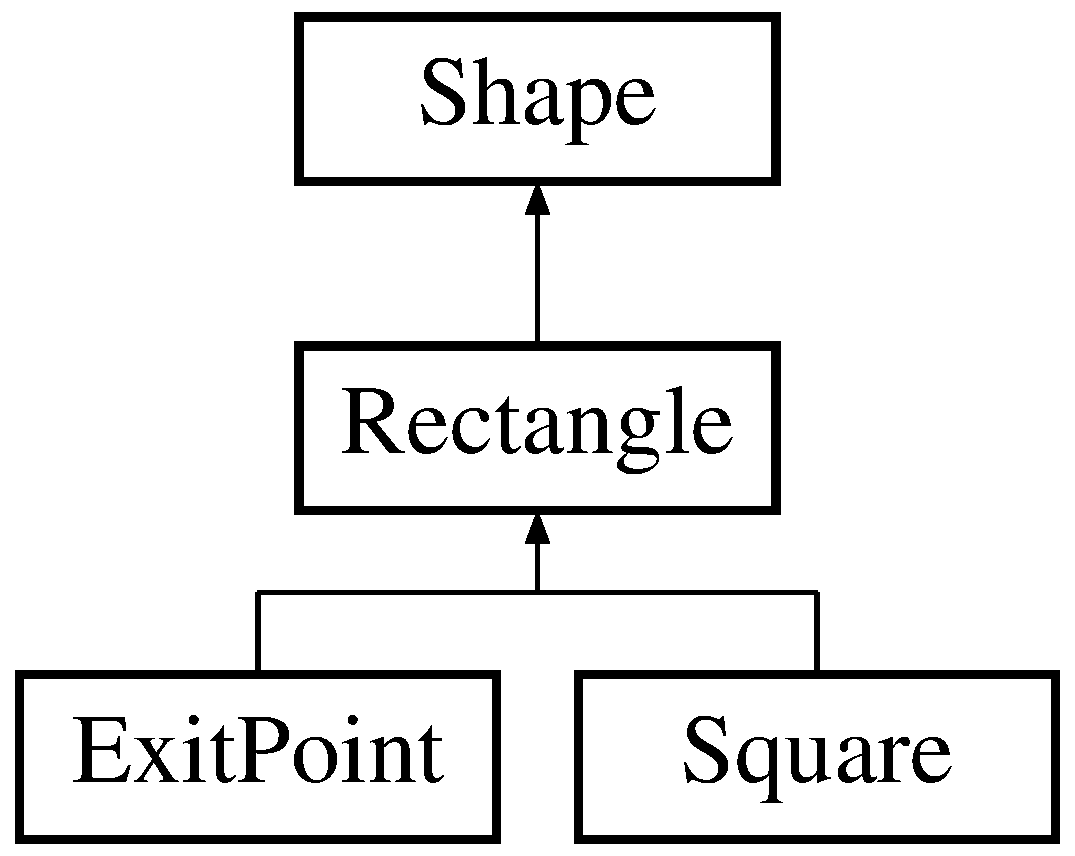
\includegraphics[height=3.000000cm]{class_rectangle}
\end{center}
\end{figure}
\subsection*{Public Member Functions}
\begin{DoxyCompactItemize}
\item 
\mbox{\hyperlink{class_rectangle_a8a933e0ebd9e80ce91e61ffe87fd577e}{Rectangle}} ()
\item 
\mbox{\hyperlink{class_rectangle_a494c076b13aadf26efdce07d23c61ddd}{$\sim$\+Rectangle}} ()
\item 
std\+::vector$<$ cv\+::\+Point $>$ \mbox{\hyperlink{class_rectangle_ae250a28affce22b4a363d1a0213df9fa}{get\+Corners}} ()
\item 
void \mbox{\hyperlink{class_rectangle_abd4c59ad5fa7010563f2efb95c553b24}{set\+Corners}} (std\+::vector$<$ cv\+::\+Point $>$ corners)
\item 
\mbox{\Hypertarget{class_rectangle_a679fadb201becac2a2eb45a689426ab0}\label{class_rectangle_a679fadb201becac2a2eb45a689426ab0}} 
cv\+::\+Point {\bfseries get\+Top\+Left} ()
\item 
\mbox{\Hypertarget{class_rectangle_a2e4b7aa32ed159fe44e580d6add40e26}\label{class_rectangle_a2e4b7aa32ed159fe44e580d6add40e26}} 
void {\bfseries set\+Top\+Left} (cv\+::\+Point top\+Left)
\item 
\mbox{\Hypertarget{class_rectangle_a2591c940d45e3449f63f95eb13c0aba1}\label{class_rectangle_a2591c940d45e3449f63f95eb13c0aba1}} 
cv\+::\+Point {\bfseries get\+Top\+Right} ()
\item 
\mbox{\Hypertarget{class_rectangle_a529ad55b3f154a231b6aad0162d8430f}\label{class_rectangle_a529ad55b3f154a231b6aad0162d8430f}} 
void {\bfseries set\+Top\+Right} (cv\+::\+Point top\+Right)
\item 
\mbox{\Hypertarget{class_rectangle_a33b9ffde2e54e9577cb369a59e965adc}\label{class_rectangle_a33b9ffde2e54e9577cb369a59e965adc}} 
cv\+::\+Point {\bfseries get\+Bottom\+Left} ()
\item 
\mbox{\Hypertarget{class_rectangle_ab393bd8f13ec5b90ed02f8d246f03ec0}\label{class_rectangle_ab393bd8f13ec5b90ed02f8d246f03ec0}} 
void {\bfseries set\+Bottom\+Left} (cv\+::\+Point bottom\+Left)
\item 
\mbox{\Hypertarget{class_rectangle_a5b5aa3a6581a32dd9e2cfc27dbda4229}\label{class_rectangle_a5b5aa3a6581a32dd9e2cfc27dbda4229}} 
cv\+::\+Point {\bfseries get\+Bottom\+Right} ()
\item 
\mbox{\Hypertarget{class_rectangle_af5cf0dfffa35328bf5d7e890d0363354}\label{class_rectangle_af5cf0dfffa35328bf5d7e890d0363354}} 
void {\bfseries set\+Bottom\+Right} (cv\+::\+Point bottom\+Right)
\item 
\mbox{\Hypertarget{class_rectangle_ac88c4a06b2688500d1209957eba41335}\label{class_rectangle_ac88c4a06b2688500d1209957eba41335}} 
void {\bfseries find\+Half} (int \&half\+\_\+h, int \&half\+\_\+w, const std\+::vector$<$ cv\+::\+Point $>$ \&corners)
\end{DoxyCompactItemize}
\subsection*{Public Attributes}
\begin{DoxyCompactItemize}
\item 
\mbox{\Hypertarget{class_rectangle_a705f4807bb92477bef644fcd63ed6c20}\label{class_rectangle_a705f4807bb92477bef644fcd63ed6c20}} 
cv\+::\+Point {\bfseries top\+\_\+left}
\item 
\mbox{\Hypertarget{class_rectangle_aa6c87573306e8ee0a7470350bfe2a17f}\label{class_rectangle_aa6c87573306e8ee0a7470350bfe2a17f}} 
cv\+::\+Point {\bfseries top\+\_\+right}
\item 
\mbox{\Hypertarget{class_rectangle_a5d2107189bd36969453560dce722ce6d}\label{class_rectangle_a5d2107189bd36969453560dce722ce6d}} 
cv\+::\+Point {\bfseries bottom\+\_\+left}
\item 
\mbox{\Hypertarget{class_rectangle_a6ed1f4dfabeb0930b864e08fb5be5915}\label{class_rectangle_a6ed1f4dfabeb0930b864e08fb5be5915}} 
cv\+::\+Point {\bfseries bottom\+\_\+right}
\end{DoxyCompactItemize}


\subsection{Detailed Description}
Class for handling square in the map. 

\subsection{Constructor \& Destructor Documentation}
\mbox{\Hypertarget{class_rectangle_a8a933e0ebd9e80ce91e61ffe87fd577e}\label{class_rectangle_a8a933e0ebd9e80ce91e61ffe87fd577e}} 
\index{Rectangle@{Rectangle}!Rectangle@{Rectangle}}
\index{Rectangle@{Rectangle}!Rectangle@{Rectangle}}
\subsubsection{\texorpdfstring{Rectangle()}{Rectangle()}}
{\footnotesize\ttfamily Rectangle\+::\+Rectangle (\begin{DoxyParamCaption}{ }\end{DoxyParamCaption})}

constructor of square class \mbox{\Hypertarget{class_rectangle_a494c076b13aadf26efdce07d23c61ddd}\label{class_rectangle_a494c076b13aadf26efdce07d23c61ddd}} 
\index{Rectangle@{Rectangle}!````~Rectangle@{$\sim$\+Rectangle}}
\index{````~Rectangle@{$\sim$\+Rectangle}!Rectangle@{Rectangle}}
\subsubsection{\texorpdfstring{$\sim$\+Rectangle()}{~Rectangle()}}
{\footnotesize\ttfamily Rectangle\+::$\sim$\+Rectangle (\begin{DoxyParamCaption}{ }\end{DoxyParamCaption})}

destructor of square class 

\subsection{Member Function Documentation}
\mbox{\Hypertarget{class_rectangle_ae250a28affce22b4a363d1a0213df9fa}\label{class_rectangle_ae250a28affce22b4a363d1a0213df9fa}} 
\index{Rectangle@{Rectangle}!get\+Corners@{get\+Corners}}
\index{get\+Corners@{get\+Corners}!Rectangle@{Rectangle}}
\subsubsection{\texorpdfstring{get\+Corners()}{getCorners()}}
{\footnotesize\ttfamily std\+::vector$<$cv\+::\+Point$>$ Rectangle\+::get\+Corners (\begin{DoxyParamCaption}{ }\end{DoxyParamCaption})}

return the list of corners \begin{DoxyReturn}{Returns}
the list of corners 
\end{DoxyReturn}
\mbox{\Hypertarget{class_rectangle_abd4c59ad5fa7010563f2efb95c553b24}\label{class_rectangle_abd4c59ad5fa7010563f2efb95c553b24}} 
\index{Rectangle@{Rectangle}!set\+Corners@{set\+Corners}}
\index{set\+Corners@{set\+Corners}!Rectangle@{Rectangle}}
\subsubsection{\texorpdfstring{set\+Corners()}{setCorners()}}
{\footnotesize\ttfamily void Rectangle\+::set\+Corners (\begin{DoxyParamCaption}\item[{std\+::vector$<$ cv\+::\+Point $>$}]{corners }\end{DoxyParamCaption})}


\begin{DoxyParams}{Parameters}
{\em corners} & return the list of corners \\
\hline
\end{DoxyParams}


The documentation for this class was generated from the following file\+:\begin{DoxyCompactItemize}
\item 
Rectangle.\+hpp\end{DoxyCompactItemize}

\hypertarget{class_robot}{}\section{Robot Class Reference}
\label{class_robot}\index{Robot@{Robot}}
Inheritance diagram for Robot\+:\begin{figure}[H]
\begin{center}
\leavevmode
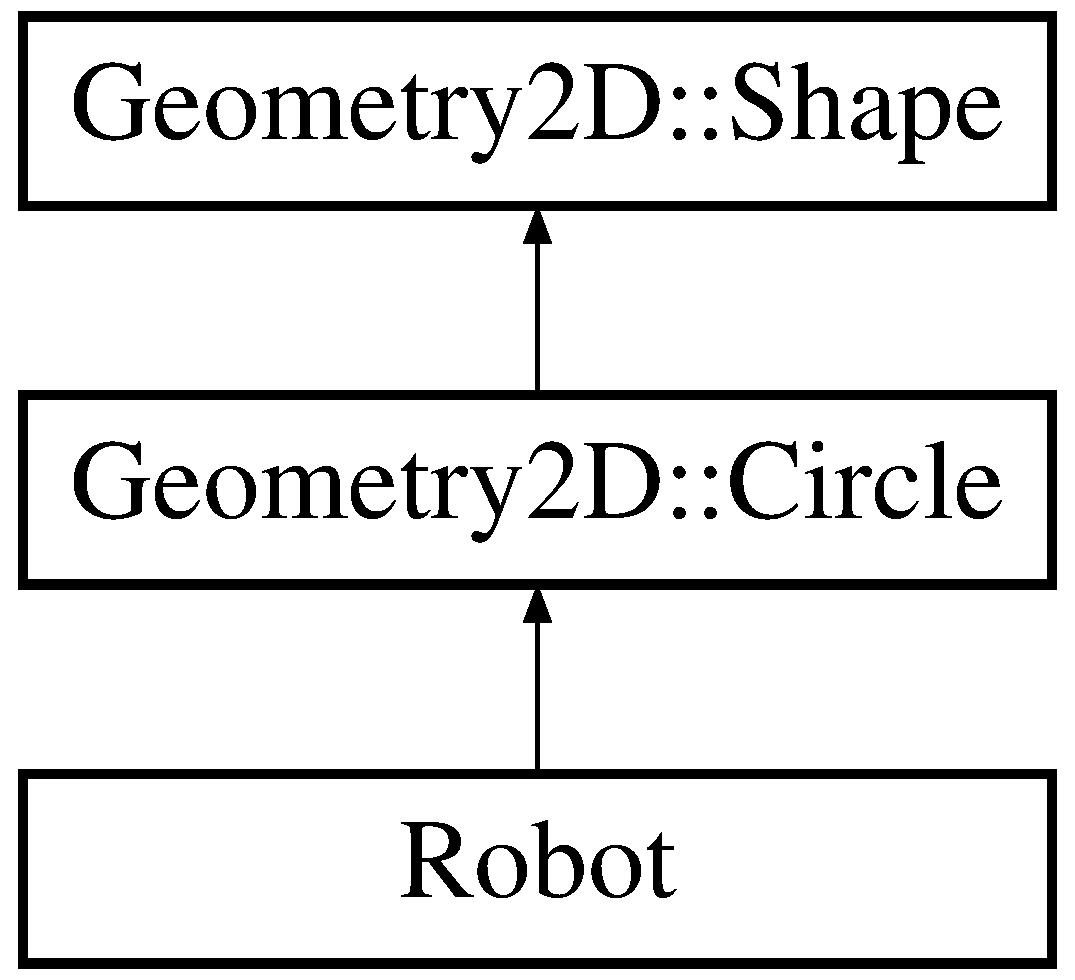
\includegraphics[height=3.000000cm]{class_robot}
\end{center}
\end{figure}
\subsection*{Public Member Functions}
\begin{DoxyCompactItemize}
\item 
\mbox{\Hypertarget{class_robot_a80c1083dea6724f840e7900210359f2a}\label{class_robot_a80c1083dea6724f840e7900210359f2a}} 
\mbox{\hyperlink{class_path_coordinates}{Path\+Coordinates}} {\bfseries initialize} ()
\end{DoxyCompactItemize}
\subsection*{Public Attributes}
\begin{DoxyCompactItemize}
\item 
\mbox{\Hypertarget{class_robot_a8f89b1b5df8f5e247e608787923fe06c}\label{class_robot_a8f89b1b5df8f5e247e608787923fe06c}} 
const cv\+::\+Scalar {\bfseries color} = cv\+::\+Scalar(0,0,255)
\item 
\mbox{\Hypertarget{class_robot_a0bda826aa4ed4fd9508fdbe02648d123}\label{class_robot_a0bda826aa4ed4fd9508fdbe02648d123}} 
\mbox{\hyperlink{class_path_coordinates}{Path\+Coordinates}} $\ast$ {\bfseries data}
\end{DoxyCompactItemize}


The documentation for this class was generated from the following file\+:\begin{DoxyCompactItemize}
\item 
Robot.\+hpp\end{DoxyCompactItemize}

\hypertarget{class_settings}{}\section{Settings Class Reference}
\label{class_settings}\index{Settings@{Settings}}
\subsection*{Public Types}
\begin{DoxyCompactItemize}
\item 
\mbox{\Hypertarget{class_settings_a0e7117abd9427a6f8bc1d1d8d456b5c8}\label{class_settings_a0e7117abd9427a6f8bc1d1d8d456b5c8}} 
enum {\bfseries Pattern} \{ {\bfseries N\+O\+T\+\_\+\+E\+X\+I\+S\+T\+I\+NG}, 
{\bfseries C\+H\+E\+S\+S\+B\+O\+A\+RD}, 
{\bfseries C\+I\+R\+C\+L\+E\+S\+\_\+\+G\+R\+ID}, 
{\bfseries A\+S\+Y\+M\+M\+E\+T\+R\+I\+C\+\_\+\+C\+I\+R\+C\+L\+E\+S\+\_\+\+G\+R\+ID}
 \}
\item 
\mbox{\Hypertarget{class_settings_a5afe85d24b071973a7f248c05386f7f4}\label{class_settings_a5afe85d24b071973a7f248c05386f7f4}} 
enum {\bfseries Input\+Type} \{ {\bfseries I\+N\+V\+A\+L\+ID}, 
{\bfseries C\+A\+M\+E\+RA}, 
{\bfseries V\+I\+D\+E\+O\+\_\+\+F\+I\+LE}, 
{\bfseries I\+M\+A\+G\+E\+\_\+\+L\+I\+ST}
 \}
\end{DoxyCompactItemize}
\subsection*{Public Member Functions}
\begin{DoxyCompactItemize}
\item 
\mbox{\Hypertarget{class_settings_a0785cc2055091b2a857b1dcefe291acc}\label{class_settings_a0785cc2055091b2a857b1dcefe291acc}} 
void {\bfseries write} (File\+Storage \&fs) const
\item 
\mbox{\Hypertarget{class_settings_a2d7841f8441095032e0f3b7d20adfd3f}\label{class_settings_a2d7841f8441095032e0f3b7d20adfd3f}} 
void {\bfseries read} (const File\+Node \&node)
\item 
\mbox{\Hypertarget{class_settings_a29016205c90b95d6247df18365a70dd0}\label{class_settings_a29016205c90b95d6247df18365a70dd0}} 
void {\bfseries validate} ()
\item 
\mbox{\Hypertarget{class_settings_a7701462e928f2425b342440fba9973e5}\label{class_settings_a7701462e928f2425b342440fba9973e5}} 
Mat {\bfseries next\+Image} ()
\end{DoxyCompactItemize}
\subsection*{Static Public Member Functions}
\begin{DoxyCompactItemize}
\item 
\mbox{\Hypertarget{class_settings_a67f01f62ca469d9ed75794079eb53c9d}\label{class_settings_a67f01f62ca469d9ed75794079eb53c9d}} 
static bool {\bfseries read\+String\+List} (const std\+::string \&filename, std\+::vector$<$ std\+::string $>$ \&l)
\item 
\mbox{\Hypertarget{class_settings_aa69f25fc79fe1dd05d990dade16669ea}\label{class_settings_aa69f25fc79fe1dd05d990dade16669ea}} 
static bool {\bfseries is\+List\+Of\+Images} (const std\+::string \&filename)
\end{DoxyCompactItemize}
\subsection*{Public Attributes}
\begin{DoxyCompactItemize}
\item 
\mbox{\Hypertarget{class_settings_a5030a7164df923bb3b86dd7a0fc9af30}\label{class_settings_a5030a7164df923bb3b86dd7a0fc9af30}} 
Size {\bfseries board\+Size}
\item 
\mbox{\Hypertarget{class_settings_a94551b7ffe8ac60311b035b2905e9498}\label{class_settings_a94551b7ffe8ac60311b035b2905e9498}} 
Pattern {\bfseries calibration\+Pattern}
\item 
\mbox{\Hypertarget{class_settings_a6c94708776ad1ce258fc44f2101f5941}\label{class_settings_a6c94708776ad1ce258fc44f2101f5941}} 
float {\bfseries square\+Size}
\item 
\mbox{\Hypertarget{class_settings_a7e6654cd0e51791ed687eaa85f8fc143}\label{class_settings_a7e6654cd0e51791ed687eaa85f8fc143}} 
int {\bfseries nr\+Frames}
\item 
\mbox{\Hypertarget{class_settings_af55c910308a0d773055d0b19261bb3b8}\label{class_settings_af55c910308a0d773055d0b19261bb3b8}} 
float {\bfseries aspect\+Ratio}
\item 
\mbox{\Hypertarget{class_settings_a5fe947366441009187d633f9e4663256}\label{class_settings_a5fe947366441009187d633f9e4663256}} 
int {\bfseries delay}
\item 
\mbox{\Hypertarget{class_settings_a53ac449815682c6bfae7e50944ba0565}\label{class_settings_a53ac449815682c6bfae7e50944ba0565}} 
bool {\bfseries write\+Points}
\item 
\mbox{\Hypertarget{class_settings_a1cee56847e08f49c90d2f7e2b0511197}\label{class_settings_a1cee56847e08f49c90d2f7e2b0511197}} 
bool {\bfseries write\+Extrinsics}
\item 
\mbox{\Hypertarget{class_settings_a4bc7ff147d74721a3587ce6fcb64ef32}\label{class_settings_a4bc7ff147d74721a3587ce6fcb64ef32}} 
bool {\bfseries calib\+Zero\+Tangent\+Dist}
\item 
\mbox{\Hypertarget{class_settings_a44397eea3f08a0c78808c38bdd716594}\label{class_settings_a44397eea3f08a0c78808c38bdd716594}} 
bool {\bfseries calib\+Fix\+Principal\+Point}
\item 
\mbox{\Hypertarget{class_settings_ab6304f260b315d2820f755e1c3a052b5}\label{class_settings_ab6304f260b315d2820f755e1c3a052b5}} 
bool {\bfseries flip\+Vertical}
\item 
\mbox{\Hypertarget{class_settings_ab2fec20428d21ea867cc044c0a583cf1}\label{class_settings_ab2fec20428d21ea867cc044c0a583cf1}} 
std\+::string {\bfseries output\+File\+Name}
\item 
\mbox{\Hypertarget{class_settings_a935d6f27ee454e9fee63f8b662f48a06}\label{class_settings_a935d6f27ee454e9fee63f8b662f48a06}} 
bool {\bfseries show\+Undistorsed}
\item 
\mbox{\Hypertarget{class_settings_a8696deae231b0efe48f1d069a4145ee6}\label{class_settings_a8696deae231b0efe48f1d069a4145ee6}} 
std\+::string {\bfseries input}
\item 
\mbox{\Hypertarget{class_settings_ac8f271630d54f9d0c718ea0130972d44}\label{class_settings_ac8f271630d54f9d0c718ea0130972d44}} 
bool {\bfseries use\+Fisheye}
\item 
\mbox{\Hypertarget{class_settings_a25242813ee2c5e111ce48fe1f7f85e7b}\label{class_settings_a25242813ee2c5e111ce48fe1f7f85e7b}} 
bool {\bfseries fix\+K1}
\item 
\mbox{\Hypertarget{class_settings_abad0b643dc5a39d493a6343d38f41578}\label{class_settings_abad0b643dc5a39d493a6343d38f41578}} 
bool {\bfseries fix\+K2}
\item 
\mbox{\Hypertarget{class_settings_a433fca3c377d42f1c7d43e35a286913f}\label{class_settings_a433fca3c377d42f1c7d43e35a286913f}} 
bool {\bfseries fix\+K3}
\item 
\mbox{\Hypertarget{class_settings_ac993998a56cebe0593cb74fe39858d31}\label{class_settings_ac993998a56cebe0593cb74fe39858d31}} 
bool {\bfseries fix\+K4}
\item 
\mbox{\Hypertarget{class_settings_a4d0d37eef5f3033a8aabc3f09ee29a03}\label{class_settings_a4d0d37eef5f3033a8aabc3f09ee29a03}} 
bool {\bfseries fix\+K5}
\item 
\mbox{\Hypertarget{class_settings_af32a5ff06192bde106c934e0361bcd7e}\label{class_settings_af32a5ff06192bde106c934e0361bcd7e}} 
int {\bfseries camera\+ID}
\item 
\mbox{\Hypertarget{class_settings_ab3f8f916639b93c3b5079facfe395078}\label{class_settings_ab3f8f916639b93c3b5079facfe395078}} 
std\+::vector$<$ std\+::string $>$ {\bfseries image\+List}
\item 
\mbox{\Hypertarget{class_settings_a1b89e85a2638e19f2d53269245d19b66}\label{class_settings_a1b89e85a2638e19f2d53269245d19b66}} 
size\+\_\+t {\bfseries at\+Image\+List}
\item 
\mbox{\Hypertarget{class_settings_abd5706146b34d3c32aef4025dcd2ec1b}\label{class_settings_abd5706146b34d3c32aef4025dcd2ec1b}} 
Video\+Capture {\bfseries input\+Capture}
\item 
\mbox{\Hypertarget{class_settings_a89fb14ce9856fb642f18bb0f7c5b8868}\label{class_settings_a89fb14ce9856fb642f18bb0f7c5b8868}} 
Input\+Type {\bfseries input\+Type}
\item 
\mbox{\Hypertarget{class_settings_a3b9fc27b555f982bd5b9ea5198e1f7e3}\label{class_settings_a3b9fc27b555f982bd5b9ea5198e1f7e3}} 
bool {\bfseries good\+Input}
\item 
\mbox{\Hypertarget{class_settings_aba5691e3e76525f93ea254e654ec3717}\label{class_settings_aba5691e3e76525f93ea254e654ec3717}} 
int {\bfseries flag}
\end{DoxyCompactItemize}


The documentation for this class was generated from the following file\+:\begin{DoxyCompactItemize}
\item 
Settings.\+hpp\end{DoxyCompactItemize}

\hypertarget{class_shape}{}\section{Shape Class Reference}
\label{class_shape}\index{Shape@{Shape}}


class for handling all the shapes in the map  




{\ttfamily \#include $<$Shape.\+hpp$>$}

Inheritance diagram for Shape\+:\begin{figure}[H]
\begin{center}
\leavevmode
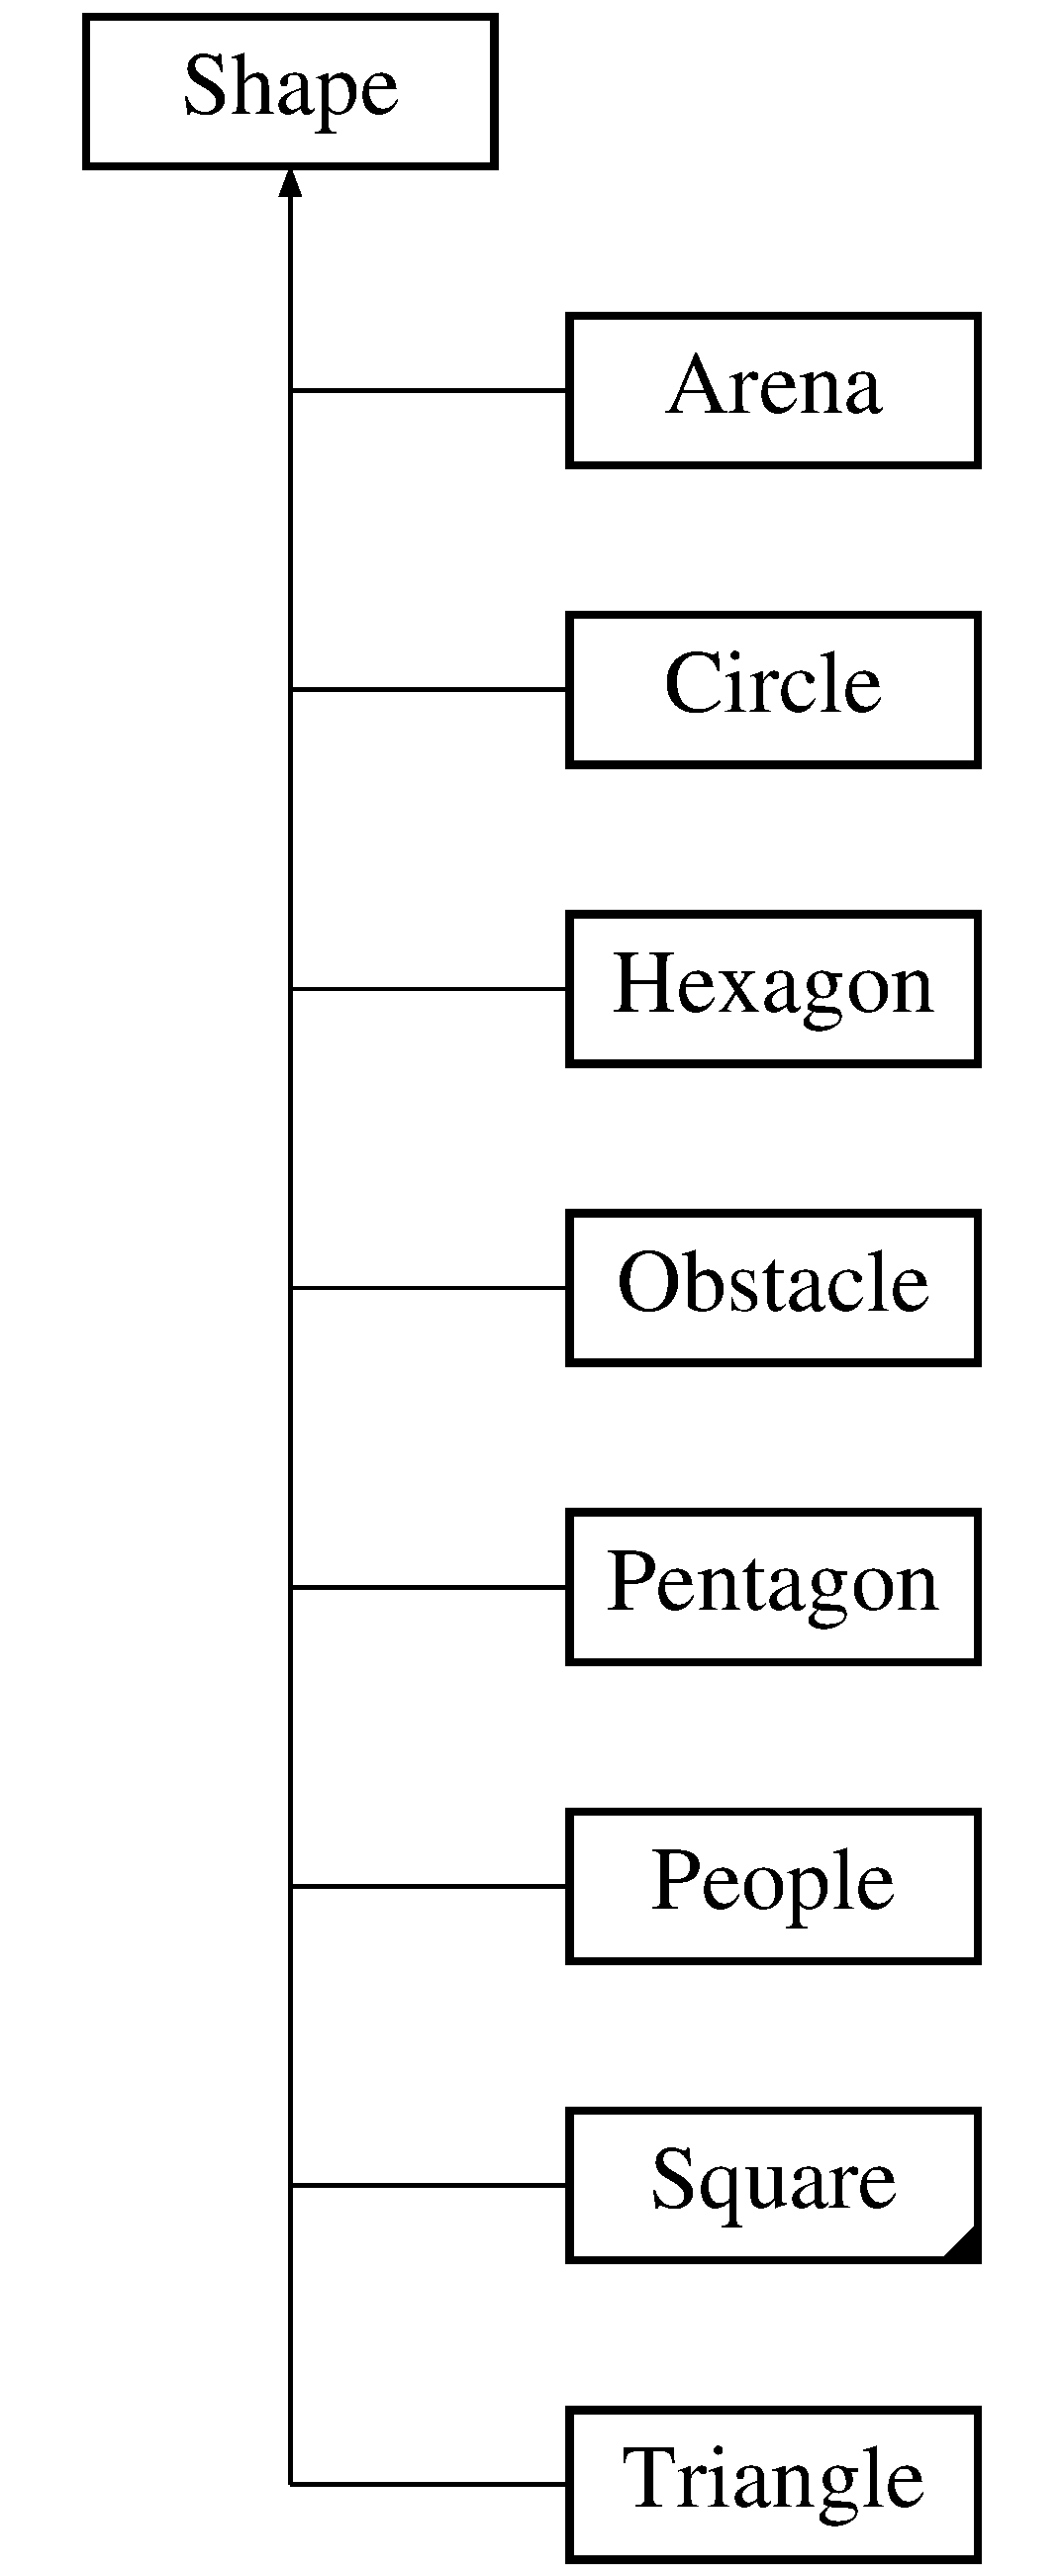
\includegraphics[height=10.000000cm]{class_shape}
\end{center}
\end{figure}
\subsection*{Public Member Functions}
\begin{DoxyCompactItemize}
\item 
\mbox{\hyperlink{class_shape_aaa8d87171e65e0d8ba3c5459978992a7}{Shape}} ()
\item 
\mbox{\hyperlink{class_shape_a935afc9e576015f967d90de56977167d}{$\sim$\+Shape}} ()
\item 
void \mbox{\hyperlink{class_shape_a9f07382e9173d32feaa737fe57560c9c}{set\+Cell}} (\mbox{\hyperlink{class_cell}{Cell}} cell\+\_\+i)
\item 
std\+::vector$<$ \mbox{\hyperlink{class_cell}{Cell}} $>$ \mbox{\hyperlink{class_shape_ad1951cad2df16392cab74b472020b851}{get\+Cell}} ()
\end{DoxyCompactItemize}


\subsection{Detailed Description}
class for handling all the shapes in the map 

\subsection{Constructor \& Destructor Documentation}
\mbox{\Hypertarget{class_shape_aaa8d87171e65e0d8ba3c5459978992a7}\label{class_shape_aaa8d87171e65e0d8ba3c5459978992a7}} 
\index{Shape@{Shape}!Shape@{Shape}}
\index{Shape@{Shape}!Shape@{Shape}}
\subsubsection{\texorpdfstring{Shape()}{Shape()}}
{\footnotesize\ttfamily Shape\+::\+Shape (\begin{DoxyParamCaption}{ }\end{DoxyParamCaption})}

constructor of the shape class \mbox{\Hypertarget{class_shape_a935afc9e576015f967d90de56977167d}\label{class_shape_a935afc9e576015f967d90de56977167d}} 
\index{Shape@{Shape}!````~Shape@{$\sim$\+Shape}}
\index{````~Shape@{$\sim$\+Shape}!Shape@{Shape}}
\subsubsection{\texorpdfstring{$\sim$\+Shape()}{~Shape()}}
{\footnotesize\ttfamily Shape\+::$\sim$\+Shape (\begin{DoxyParamCaption}{ }\end{DoxyParamCaption})}

destructor of the shape class 

\subsection{Member Function Documentation}
\mbox{\Hypertarget{class_shape_ad1951cad2df16392cab74b472020b851}\label{class_shape_ad1951cad2df16392cab74b472020b851}} 
\index{Shape@{Shape}!get\+Cell@{get\+Cell}}
\index{get\+Cell@{get\+Cell}!Shape@{Shape}}
\subsubsection{\texorpdfstring{get\+Cell()}{getCell()}}
{\footnotesize\ttfamily std\+::vector$<$\mbox{\hyperlink{class_cell}{Cell}}$>$ Shape\+::get\+Cell (\begin{DoxyParamCaption}{ }\end{DoxyParamCaption})}

return the cell which is connected \begin{DoxyReturn}{Returns}
the cell which is connected 
\end{DoxyReturn}
\mbox{\Hypertarget{class_shape_a9f07382e9173d32feaa737fe57560c9c}\label{class_shape_a9f07382e9173d32feaa737fe57560c9c}} 
\index{Shape@{Shape}!set\+Cell@{set\+Cell}}
\index{set\+Cell@{set\+Cell}!Shape@{Shape}}
\subsubsection{\texorpdfstring{set\+Cell()}{setCell()}}
{\footnotesize\ttfamily void Shape\+::set\+Cell (\begin{DoxyParamCaption}\item[{\mbox{\hyperlink{class_cell}{Cell}}}]{cell\+\_\+i }\end{DoxyParamCaption})}

connect a cell to the shape 
\begin{DoxyParams}{Parameters}
{\em cell\+\_\+i} & cell that has to be connected to the shape \\
\hline
\end{DoxyParams}


The documentation for this class was generated from the following file\+:\begin{DoxyCompactItemize}
\item 
Shape.\+hpp\end{DoxyCompactItemize}

\hypertarget{class_square}{}\section{Square Class Reference}
\label{class_square}\index{Square@{Square}}


{\ttfamily \#include $<$Square.\+hpp$>$}

Inheritance diagram for Square\+:\begin{figure}[H]
\begin{center}
\leavevmode
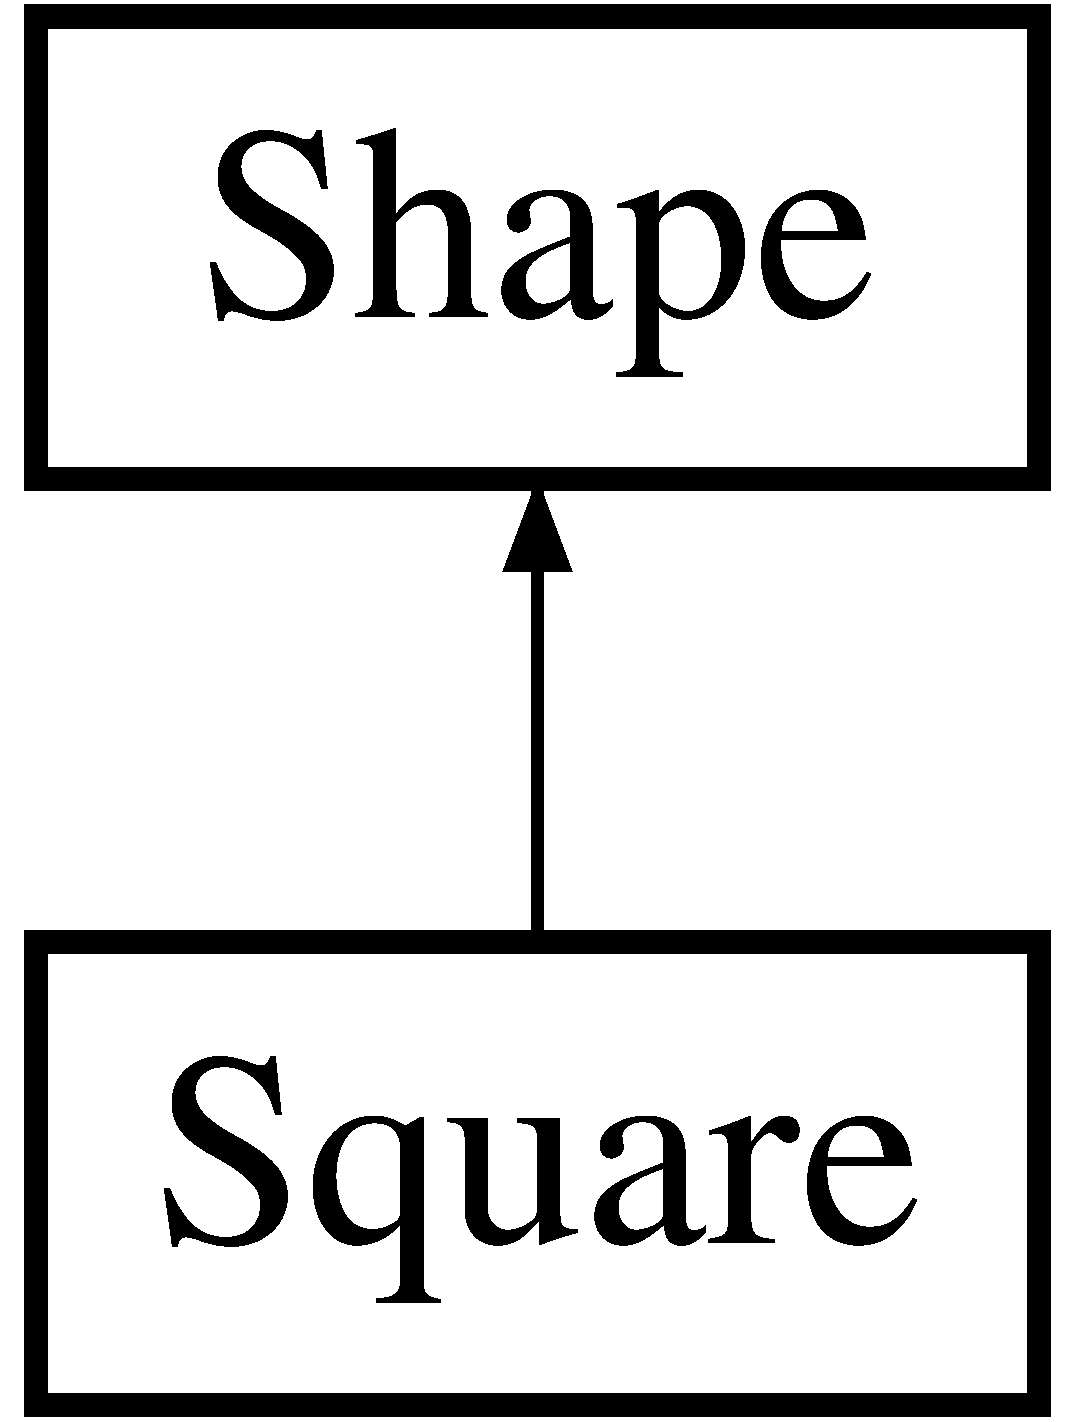
\includegraphics[height=2.000000cm]{class_square}
\end{center}
\end{figure}
\subsection*{Public Member Functions}
\begin{DoxyCompactItemize}
\item 
\mbox{\hyperlink{class_square_a3dc7ff9aefc2725172b5d3153973d243}{Square}} ()
\item 
\mbox{\hyperlink{class_square_a90af7ce1060cff7b717ceddb333846b8}{$\sim$\+Square}} ()
\item 
std\+::vector$<$ cv\+::\+Point $>$ \mbox{\hyperlink{class_square_a53b1e1223e97676db711dd75f2daa508}{get\+Corners}} ()
\item 
void \mbox{\hyperlink{class_square_a84c4995b49318b5191a4fe3739e4f081}{set\+Corners}} (std\+::vector$<$ cv\+::\+Point $>$ corners)
\end{DoxyCompactItemize}


\subsection{Detailed Description}
Class for handling square in the map 

\subsection{Constructor \& Destructor Documentation}
\mbox{\Hypertarget{class_square_a3dc7ff9aefc2725172b5d3153973d243}\label{class_square_a3dc7ff9aefc2725172b5d3153973d243}} 
\index{Square@{Square}!Square@{Square}}
\index{Square@{Square}!Square@{Square}}
\subsubsection{\texorpdfstring{Square()}{Square()}}
{\footnotesize\ttfamily Square\+::\+Square (\begin{DoxyParamCaption}{ }\end{DoxyParamCaption})}

constructor of square class \mbox{\Hypertarget{class_square_a90af7ce1060cff7b717ceddb333846b8}\label{class_square_a90af7ce1060cff7b717ceddb333846b8}} 
\index{Square@{Square}!````~Square@{$\sim$\+Square}}
\index{````~Square@{$\sim$\+Square}!Square@{Square}}
\subsubsection{\texorpdfstring{$\sim$\+Square()}{~Square()}}
{\footnotesize\ttfamily Square\+::$\sim$\+Square (\begin{DoxyParamCaption}{ }\end{DoxyParamCaption})}

destructor of square class 

\subsection{Member Function Documentation}
\mbox{\Hypertarget{class_square_a53b1e1223e97676db711dd75f2daa508}\label{class_square_a53b1e1223e97676db711dd75f2daa508}} 
\index{Square@{Square}!get\+Corners@{get\+Corners}}
\index{get\+Corners@{get\+Corners}!Square@{Square}}
\subsubsection{\texorpdfstring{get\+Corners()}{getCorners()}}
{\footnotesize\ttfamily std\+::vector$<$cv\+::\+Point$>$ Square\+::get\+Corners (\begin{DoxyParamCaption}{ }\end{DoxyParamCaption})}

return the list of corners \begin{DoxyReturn}{Returns}
the list of corners 
\end{DoxyReturn}
\mbox{\Hypertarget{class_square_a84c4995b49318b5191a4fe3739e4f081}\label{class_square_a84c4995b49318b5191a4fe3739e4f081}} 
\index{Square@{Square}!set\+Corners@{set\+Corners}}
\index{set\+Corners@{set\+Corners}!Square@{Square}}
\subsubsection{\texorpdfstring{set\+Corners()}{setCorners()}}
{\footnotesize\ttfamily void Square\+::set\+Corners (\begin{DoxyParamCaption}\item[{std\+::vector$<$ cv\+::\+Point $>$}]{corners }\end{DoxyParamCaption})}


\begin{DoxyParams}{Parameters}
{\em corners} & return the list of corners \\
\hline
\end{DoxyParams}


The documentation for this class was generated from the following file\+:\begin{DoxyCompactItemize}
\item 
Square.\+hpp\end{DoxyCompactItemize}

\hypertarget{structstandard_conf}{}\section{standard\+Conf Struct Reference}
\label{structstandard_conf}\index{standard\+Conf@{standard\+Conf}}
\subsection*{Public Attributes}
\begin{DoxyCompactItemize}
\item 
\mbox{\Hypertarget{structstandard_conf_ac5a8976654eddd1c14b2aab5f4401943}\label{structstandard_conf_ac5a8976654eddd1c14b2aab5f4401943}} 
double {\bfseries lambda}
\item 
\mbox{\Hypertarget{structstandard_conf_a105f1c9c8b50dc1f82ded42d04efeddb}\label{structstandard_conf_a105f1c9c8b50dc1f82ded42d04efeddb}} 
double {\bfseries sc\+\_\+th0}
\item 
\mbox{\Hypertarget{structstandard_conf_a10bf9ad5cc1f29e5414bcad2d762273c}\label{structstandard_conf_a10bf9ad5cc1f29e5414bcad2d762273c}} 
double {\bfseries sc\+\_\+thf}
\item 
\mbox{\Hypertarget{structstandard_conf_a394472a69fcea7d55ff5925a878e4d2d}\label{structstandard_conf_a394472a69fcea7d55ff5925a878e4d2d}} 
double {\bfseries sc\+\_\+\+Kmax}
\end{DoxyCompactItemize}


The documentation for this struct was generated from the following file\+:\begin{DoxyCompactItemize}
\item 
Dubin\+Path\+Finder.\+hpp\end{DoxyCompactItemize}

\hypertarget{class_straight_line}{}\section{Straight\+Line Class Reference}
\label{class_straight_line}\index{Straight\+Line@{Straight\+Line}}


describe a \mbox{\hyperlink{class_straight_line}{Straight\+Line}} in the path  




{\ttfamily \#include $<$Straight\+Line.\+hpp$>$}

Inheritance diagram for Straight\+Line\+:\begin{figure}[H]
\begin{center}
\leavevmode
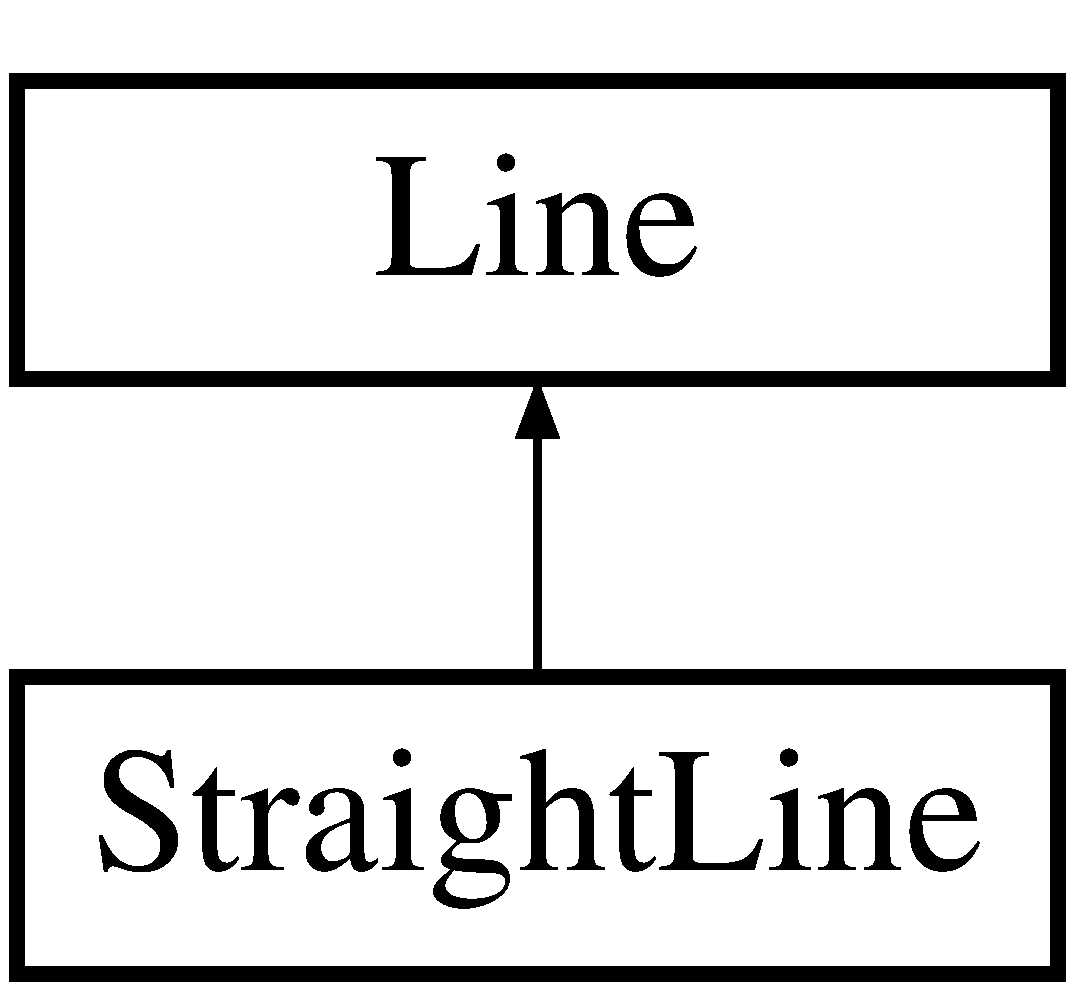
\includegraphics[height=2.000000cm]{class_straight_line}
\end{center}
\end{figure}
\subsection*{Public Member Functions}
\begin{DoxyCompactItemize}
\item 
\mbox{\hyperlink{class_straight_line_a583064766a4c73bfa58ee1cb9f5b4495}{Straight\+Line}} (\mbox{\hyperlink{class_position}{Position}} start\+\_\+point, \mbox{\hyperlink{class_position}{Position}} end\+\_\+point)
\begin{DoxyCompactList}\small\item\em constructor of the \mbox{\hyperlink{class_straight_line}{Straight\+Line}} class \end{DoxyCompactList}\item 
\mbox{\hyperlink{class_straight_line_ac55a20f7c9d8ba62f4dd0bba0e9d8c4e}{Straight\+Line}} (\mbox{\hyperlink{class_position}{Position}} start\+\_\+point, double length)
\begin{DoxyCompactList}\small\item\em constructor of the \mbox{\hyperlink{class_straight_line}{Straight\+Line}} class \end{DoxyCompactList}\item 
\mbox{\Hypertarget{class_straight_line_a24fc4b7e915d5a42b40f716e49558663}\label{class_straight_line_a24fc4b7e915d5a42b40f716e49558663}} 
\mbox{\hyperlink{class_straight_line_a24fc4b7e915d5a42b40f716e49558663}{$\sim$\+Straight\+Line}} ()
\begin{DoxyCompactList}\small\item\em destructor of the \mbox{\hyperlink{class_straight_line}{Straight\+Line}} class \end{DoxyCompactList}\end{DoxyCompactItemize}


\subsection{Detailed Description}
describe a \mbox{\hyperlink{class_straight_line}{Straight\+Line}} in the path 

\subsection{Constructor \& Destructor Documentation}
\mbox{\Hypertarget{class_straight_line_a583064766a4c73bfa58ee1cb9f5b4495}\label{class_straight_line_a583064766a4c73bfa58ee1cb9f5b4495}} 
\index{Straight\+Line@{Straight\+Line}!Straight\+Line@{Straight\+Line}}
\index{Straight\+Line@{Straight\+Line}!Straight\+Line@{Straight\+Line}}
\subsubsection{\texorpdfstring{Straight\+Line()}{StraightLine()}\hspace{0.1cm}{\footnotesize\ttfamily [1/2]}}
{\footnotesize\ttfamily Straight\+Line\+::\+Straight\+Line (\begin{DoxyParamCaption}\item[{\mbox{\hyperlink{class_position}{Position}}}]{start\+\_\+point,  }\item[{\mbox{\hyperlink{class_position}{Position}}}]{end\+\_\+point }\end{DoxyParamCaption})}



constructor of the \mbox{\hyperlink{class_straight_line}{Straight\+Line}} class 


\begin{DoxyParams}{Parameters}
{\em start\+\_\+point} & start point of the line \\
\hline
{\em end\+\_\+point} & end point of the line \\
\hline
\end{DoxyParams}
\mbox{\Hypertarget{class_straight_line_ac55a20f7c9d8ba62f4dd0bba0e9d8c4e}\label{class_straight_line_ac55a20f7c9d8ba62f4dd0bba0e9d8c4e}} 
\index{Straight\+Line@{Straight\+Line}!Straight\+Line@{Straight\+Line}}
\index{Straight\+Line@{Straight\+Line}!Straight\+Line@{Straight\+Line}}
\subsubsection{\texorpdfstring{Straight\+Line()}{StraightLine()}\hspace{0.1cm}{\footnotesize\ttfamily [2/2]}}
{\footnotesize\ttfamily Straight\+Line\+::\+Straight\+Line (\begin{DoxyParamCaption}\item[{\mbox{\hyperlink{class_position}{Position}}}]{start\+\_\+point,  }\item[{double}]{length }\end{DoxyParamCaption})}



constructor of the \mbox{\hyperlink{class_straight_line}{Straight\+Line}} class 


\begin{DoxyParams}{Parameters}
{\em start\+\_\+point} & start point of the line \\
\hline
{\em length} & length of the line \\
\hline
\end{DoxyParams}


The documentation for this class was generated from the following file\+:\begin{DoxyCompactItemize}
\item 
Straight\+Line.\+hpp\end{DoxyCompactItemize}

\hypertarget{class_template___character___recognition}{}\section{Template\+\_\+\+Character\+\_\+\+Recognition Class Reference}
\label{class_template___character___recognition}\index{Template\+\_\+\+Character\+\_\+\+Recognition@{Template\+\_\+\+Character\+\_\+\+Recognition}}
Inheritance diagram for Template\+\_\+\+Character\+\_\+\+Recognition\+:\begin{figure}[H]
\begin{center}
\leavevmode
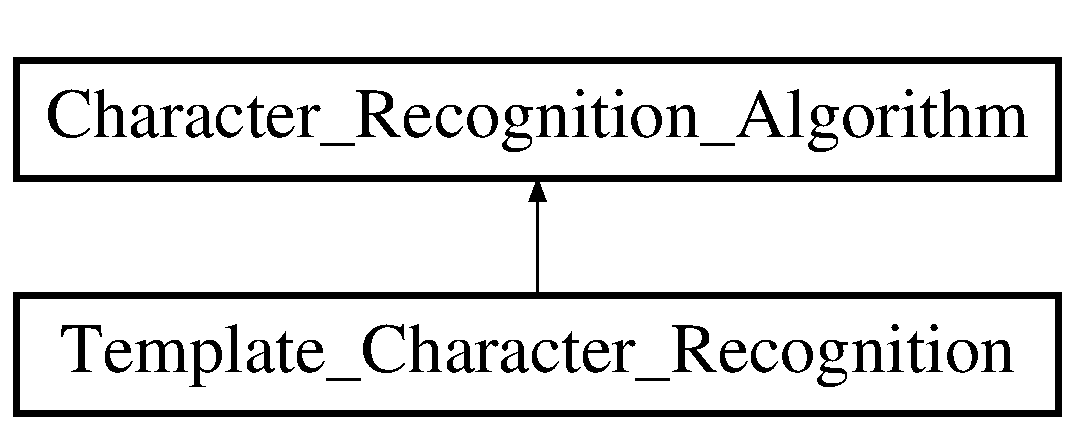
\includegraphics[height=2.000000cm]{class_template___character___recognition}
\end{center}
\end{figure}
\subsection*{Public Member Functions}
\begin{DoxyCompactItemize}
\item 
\mbox{\Hypertarget{class_template___character___recognition_af41bc392058896b69802f690e42661dc}\label{class_template___character___recognition_af41bc392058896b69802f690e42661dc}} 
std\+::pair$<$ int, int $>$ \mbox{\hyperlink{class_template___character___recognition_af41bc392058896b69802f690e42661dc}{detect\+\_\+digit}} (cv\+::\+Mat \&image)
\begin{DoxyCompactList}\small\item\em the (virtual) function that runs the recognition engine \end{DoxyCompactList}\item 
\mbox{\Hypertarget{class_template___character___recognition_a0af8778b93c92849d3413f2b3d0333bd}\label{class_template___character___recognition_a0af8778b93c92849d3413f2b3d0333bd}} 
int {\bfseries get\+Result} (std\+::vector$<$ cv\+::\+Mat $>$ \&templ\+R\+O\+Is, cv\+::\+Mat \&R\+OI)
\end{DoxyCompactItemize}
\subsection*{Public Attributes}
\begin{DoxyCompactItemize}
\item 
\mbox{\Hypertarget{class_template___character___recognition_aa4cb4d3779f7d7a65ae5811f78be880b}\label{class_template___character___recognition_aa4cb4d3779f7d7a65ae5811f78be880b}} 
const std\+::string {\bfseries template\+\_\+path} = \char`\"{}../data/template/\char`\"{}
\end{DoxyCompactItemize}


The documentation for this class was generated from the following file\+:\begin{DoxyCompactItemize}
\item 
Template\+\_\+\+Character\+\_\+\+Recognition.\+hpp\end{DoxyCompactItemize}

\hypertarget{class_triangle}{}\section{Triangle Class Reference}
\label{class_triangle}\index{Triangle@{Triangle}}


{\ttfamily \#include $<$Triangle.\+hpp$>$}

Inheritance diagram for Triangle\+:\begin{figure}[H]
\begin{center}
\leavevmode
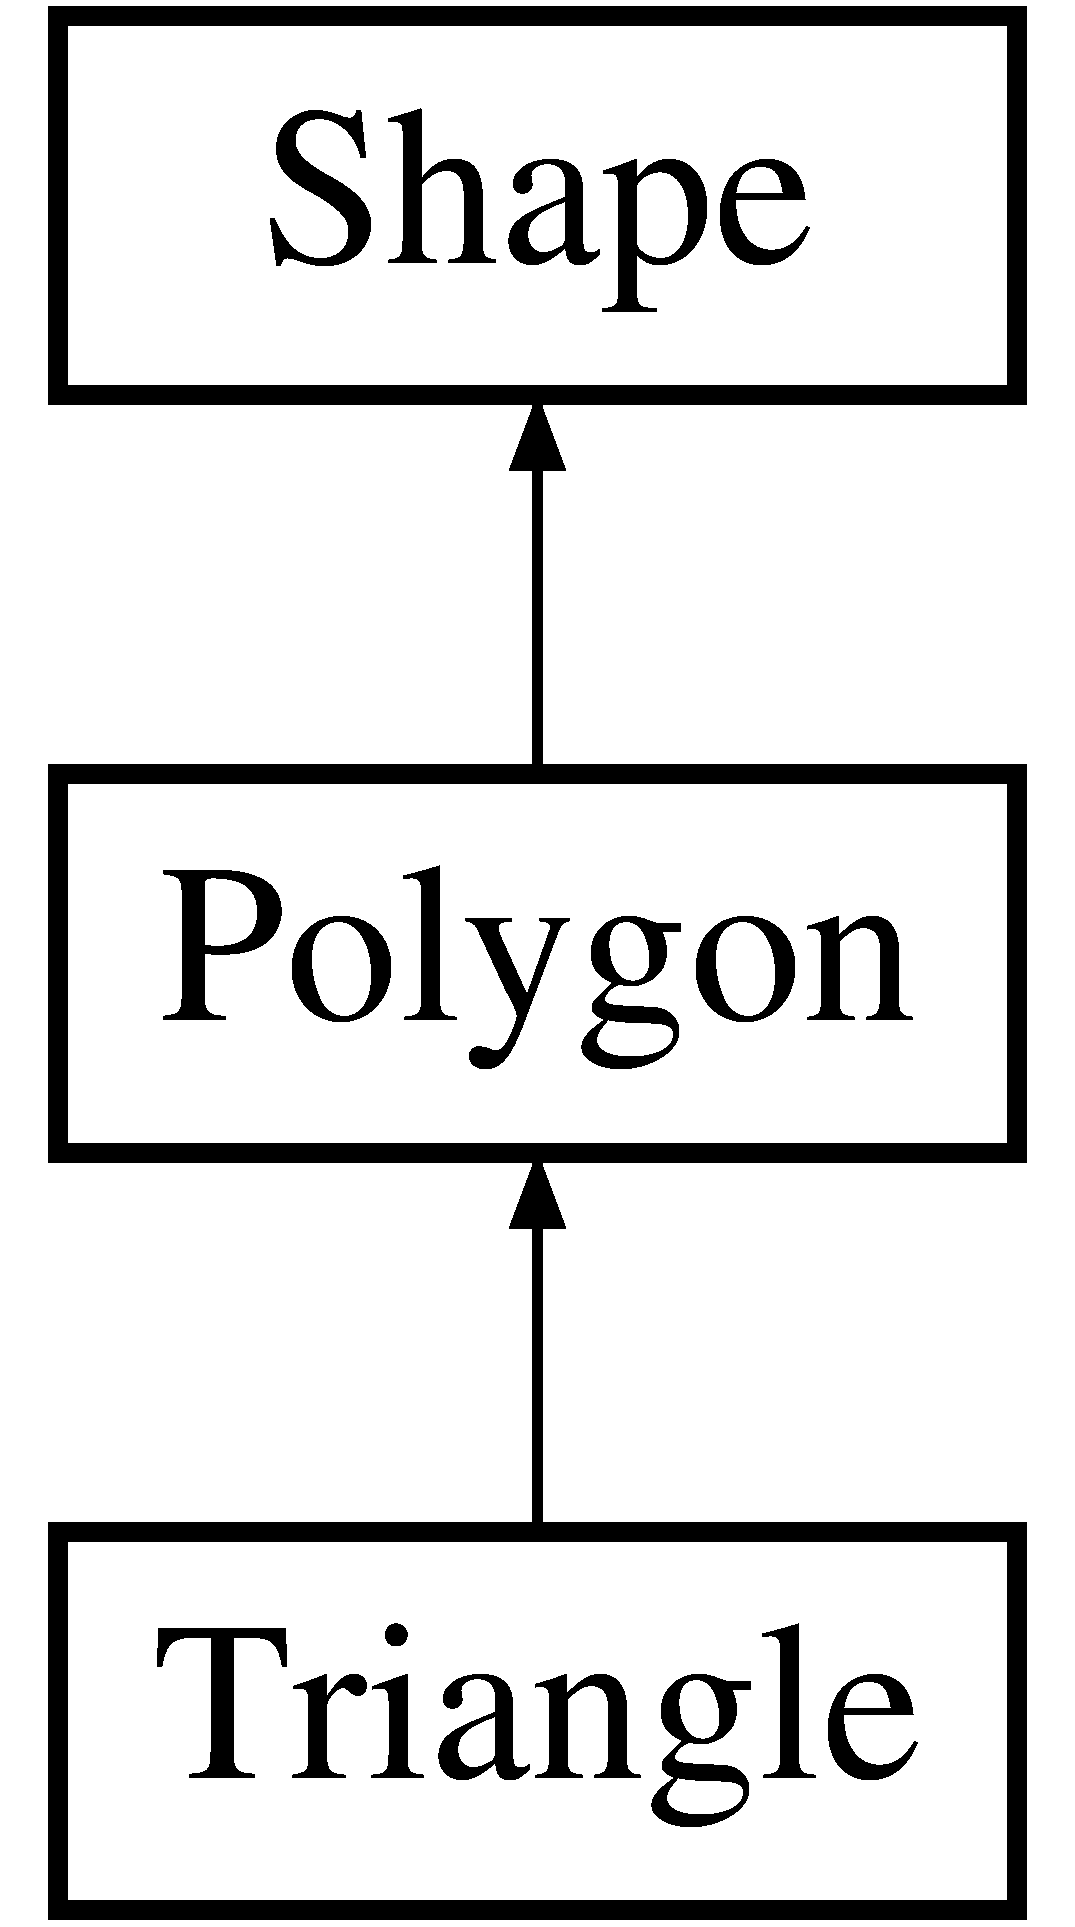
\includegraphics[height=2.000000cm]{class_triangle}
\end{center}
\end{figure}
\subsection*{Public Member Functions}
\begin{DoxyCompactItemize}
\item 
\mbox{\hyperlink{class_triangle_aaefe4ed500c07918d30c6f0e286332c5}{Triangle}} ()
\item 
\mbox{\hyperlink{class_triangle_a5199760a17454f4dc94c855a57e3a152}{$\sim$\+Triangle}} ()
\item 
std\+::vector$<$ cv\+::\+Point $>$ \mbox{\hyperlink{class_triangle_a0c77555fd0e47f1344c23fa880f43777}{get\+Corners}} ()
\item 
void \mbox{\hyperlink{class_triangle_ad2d4cecee7e87e10d8b2787199d784c2}{set\+Corners}} (std\+::vector$<$ cv\+::\+Point $>$ corners)
\end{DoxyCompactItemize}


\subsection{Detailed Description}
class for handling triangle obstacles 

\subsection{Constructor \& Destructor Documentation}
\mbox{\Hypertarget{class_triangle_aaefe4ed500c07918d30c6f0e286332c5}\label{class_triangle_aaefe4ed500c07918d30c6f0e286332c5}} 
\index{Triangle@{Triangle}!Triangle@{Triangle}}
\index{Triangle@{Triangle}!Triangle@{Triangle}}
\subsubsection{\texorpdfstring{Triangle()}{Triangle()}}
{\footnotesize\ttfamily Triangle\+::\+Triangle (\begin{DoxyParamCaption}{ }\end{DoxyParamCaption})}

constructor of triangle class \mbox{\Hypertarget{class_triangle_a5199760a17454f4dc94c855a57e3a152}\label{class_triangle_a5199760a17454f4dc94c855a57e3a152}} 
\index{Triangle@{Triangle}!````~Triangle@{$\sim$\+Triangle}}
\index{````~Triangle@{$\sim$\+Triangle}!Triangle@{Triangle}}
\subsubsection{\texorpdfstring{$\sim$\+Triangle()}{~Triangle()}}
{\footnotesize\ttfamily Triangle\+::$\sim$\+Triangle (\begin{DoxyParamCaption}{ }\end{DoxyParamCaption})}

destructor of triangle class 

\subsection{Member Function Documentation}
\mbox{\Hypertarget{class_triangle_a0c77555fd0e47f1344c23fa880f43777}\label{class_triangle_a0c77555fd0e47f1344c23fa880f43777}} 
\index{Triangle@{Triangle}!get\+Corners@{get\+Corners}}
\index{get\+Corners@{get\+Corners}!Triangle@{Triangle}}
\subsubsection{\texorpdfstring{get\+Corners()}{getCorners()}}
{\footnotesize\ttfamily std\+::vector$<$cv\+::\+Point$>$ Triangle\+::get\+Corners (\begin{DoxyParamCaption}{ }\end{DoxyParamCaption})}

return the list of corners \begin{DoxyReturn}{Returns}
list of corners of the triangle 
\end{DoxyReturn}
\mbox{\Hypertarget{class_triangle_ad2d4cecee7e87e10d8b2787199d784c2}\label{class_triangle_ad2d4cecee7e87e10d8b2787199d784c2}} 
\index{Triangle@{Triangle}!set\+Corners@{set\+Corners}}
\index{set\+Corners@{set\+Corners}!Triangle@{Triangle}}
\subsubsection{\texorpdfstring{set\+Corners()}{setCorners()}}
{\footnotesize\ttfamily void Triangle\+::set\+Corners (\begin{DoxyParamCaption}\item[{std\+::vector$<$ cv\+::\+Point $>$}]{corners }\end{DoxyParamCaption})}

set corners of the triangle 
\begin{DoxyParams}{Parameters}
{\em corners} & list of corners \\
\hline
\end{DoxyParams}


The documentation for this class was generated from the following file\+:\begin{DoxyCompactItemize}
\item 
Triangle.\+hpp\end{DoxyCompactItemize}

\hypertarget{class_undistorsion}{}\section{Undistorsion Class Reference}
\label{class_undistorsion}\index{Undistorsion@{Undistorsion}}


{\ttfamily \#include $<$Undistortion.\+hpp$>$}

\subsection*{Public Member Functions}
\begin{DoxyCompactItemize}
\item 
\mbox{\hyperlink{class_undistorsion_a447aceee5716c408a3ed662111525cf9}{Undistorsion}} (std\+::string calibration\+\_\+filename)
\item 
\mbox{\hyperlink{class_undistorsion_adc5adf65c7ee3f5668bafd8eeaf31eb4}{$\sim$\+Undistorsion}} ()
\item 
void \mbox{\hyperlink{class_undistorsion_a00c36a6d87702b119e87ca0ff003c92f}{undistort\+\_\+image}} (cv\+::\+Mat frame, cv\+::\+Mat frame\+Undist, Input\+Array camera\+Matrix, Input\+Array dist\+Coeffs, Input\+Array new\+Camera\+Matrix=no\+Array())
\end{DoxyCompactItemize}


\subsection{Detailed Description}
class for undistorsion of the images 

\subsection{Constructor \& Destructor Documentation}
\mbox{\Hypertarget{class_undistorsion_a447aceee5716c408a3ed662111525cf9}\label{class_undistorsion_a447aceee5716c408a3ed662111525cf9}} 
\index{Undistorsion@{Undistorsion}!Undistorsion@{Undistorsion}}
\index{Undistorsion@{Undistorsion}!Undistorsion@{Undistorsion}}
\subsubsection{\texorpdfstring{Undistorsion()}{Undistorsion()}}
{\footnotesize\ttfamily Undistorsion\+::\+Undistorsion (\begin{DoxyParamCaption}\item[{std\+::string}]{calibration\+\_\+filename }\end{DoxyParamCaption})}

construcor of the Undistorion class 
\begin{DoxyParams}{Parameters}
{\em calibration\+\_\+filename} & name of the calibration file \\
\hline
\end{DoxyParams}
\mbox{\Hypertarget{class_undistorsion_adc5adf65c7ee3f5668bafd8eeaf31eb4}\label{class_undistorsion_adc5adf65c7ee3f5668bafd8eeaf31eb4}} 
\index{Undistorsion@{Undistorsion}!````~Undistorsion@{$\sim$\+Undistorsion}}
\index{````~Undistorsion@{$\sim$\+Undistorsion}!Undistorsion@{Undistorsion}}
\subsubsection{\texorpdfstring{$\sim$\+Undistorsion()}{~Undistorsion()}}
{\footnotesize\ttfamily Undistorsion\+::$\sim$\+Undistorsion (\begin{DoxyParamCaption}{ }\end{DoxyParamCaption})}

destructor of the Undistortion class 

\subsection{Member Function Documentation}
\mbox{\Hypertarget{class_undistorsion_a00c36a6d87702b119e87ca0ff003c92f}\label{class_undistorsion_a00c36a6d87702b119e87ca0ff003c92f}} 
\index{Undistorsion@{Undistorsion}!undistort\+\_\+image@{undistort\+\_\+image}}
\index{undistort\+\_\+image@{undistort\+\_\+image}!Undistorsion@{Undistorsion}}
\subsubsection{\texorpdfstring{undistort\+\_\+image()}{undistort\_image()}}
{\footnotesize\ttfamily void Undistorsion\+::undistort\+\_\+image (\begin{DoxyParamCaption}\item[{cv\+::\+Mat}]{frame,  }\item[{cv\+::\+Mat}]{frame\+Undist,  }\item[{Input\+Array}]{camera\+Matrix,  }\item[{Input\+Array}]{dist\+Coeffs,  }\item[{Input\+Array}]{new\+Camera\+Matrix = {\ttfamily noArray()} }\end{DoxyParamCaption})}

function that undistort the image 
\begin{DoxyParams}{Parameters}
{\em frame} & \\
\hline
{\em frame\+Undist} & \\
\hline
{\em camera\+Matrix} & \\
\hline
{\em dist\+Coeffs} & \\
\hline
{\em new\+Camera\+Matrix} & \\
\hline
\end{DoxyParams}


The documentation for this class was generated from the following file\+:\begin{DoxyCompactItemize}
\item 
Undistortion.\+hpp\end{DoxyCompactItemize}

%--- End generated contents ---

% Index
\backmatter
\newpage
\phantomsection
\clearemptydoublepage
\addcontentsline{toc}{chapter}{Index}
\printindex

\end{document}
